\documentclass[12pt,a4paper]{article}
\usepackage[utf8]{inputenc}
\usepackage[T1]{fontenc}
\usepackage{geometry}
\usepackage{graphicx}
\usepackage{float}
\usepackage{longtable}
\usepackage{booktabs}
\usepackage{array}
\usepackage{multirow}
\usepackage{wrapfig}
\usepackage{rotating}
\usepackage{listings}
\usepackage{color}
\usepackage{enumitem}
\usepackage{hyperref}
\usepackage{fancyhdr}
\usepackage{titlesec}
\usepackage{setspace}
\usepackage{parskip}
\usepackage[english]{babel}
\usepackage{subcaption}
\usepackage{url}
\setlength{\headheight}{15pt}
\addtolength{\topmargin}{-3pt}

% Page setup
\geometry{margin=1in}
\setlength{\parindent}{0pt}
\setlength{\parskip}{6pt}

% Header and footer
\pagestyle{fancy}
\fancyhf{}
\fancyhead[L]{\textbf{Vacation Management System - SRS}}
\fancyhead[R]{\thepage}
\renewcommand{\headrulewidth}{0.4pt}

% Title formatting
\titleformat{\section}{\Large\bfseries}{\thesection}{1em}{}
\titleformat{\subsection}{\large\bfseries}{\thesubsection}{1em}{}
\titleformat{\subsubsection}{\normalsize\bfseries}{\thesubsubsection}{1em}{}

% Custom colors
\definecolor{codegreen}{rgb}{0,0.6,0}
\definecolor{codegray}{rgb}{0.5,0.5,0.5}
\definecolor{codepurple}{rgb}{0.58,0,0.82}
\definecolor{backcolour}{rgb}{0.95,0.95,0.92}

% Code listing style
\lstdefinestyle{mystyle}{
    backgroundcolor=\color{backcolour},   
    commentstyle=\color{codegreen},
    keywordstyle=\color{magenta},
    numberstyle=\tiny\color{codegray},
    stringstyle=\color{codepurple},
    basicstyle=\ttfamily\footnotesize,
    breakatwhitespace=false,         
    breaklines=true,                 
    captionpos=b,                    
    keepspaces=true,                 
    numbers=left,                    
    numbersep=5pt,                  
    showspaces=false,                
    showstringspaces=false,
    showtabs=false,                  
    tabsize=2
}
\lstset{style=mystyle}

% Table style
\newcolumntype{P}[1]{>{\centering\arraybackslash}p{#1}}

\begin{document}

% Title Page
\begin{titlepage}
\centering
\vspace*{2cm}
{\Huge\bfseries Vacation Management System\par}
\vspace{1cm}
{\Large\bfseries Software Requirements Specification\par}
\vspace{2cm}
{\large Version 2.0\par}
\vspace{1cm}
{\large \today\par}
\vspace{2cm}
{\large Prepared for: Ejada\par}
\vspace{1cm}
{\large Prepared by: Omar Abdelrahman Abbas\par}
\vspace{1cm}
{\large Under supervision of: Ahmed Abdelwahab Mohamed\par}
\vspace{1cm}
{\large Document Type: Software Requirements Specification\par}
\vfill
\end{titlepage}

% Table of Contents
\tableofcontents
\newpage

% List of Figures
\listoffigures
\newpage

% List of Tables
\listoftables
\newpage

\section{Introduction}

\subsection{Purpose}
This Software Requirements Specification (SRS) document describes the functional and non-functional requirements for the Vacation Management System. The document serves as a comprehensive contract between the development team and stakeholders, providing a detailed understanding of what the system should accomplish based on the complete project scope and use cases.

\subsection{Scope}
The Vacation Management System is designed to automate the vacation request, approval, and cancellation processes while providing robust reporting capabilities for efficient vacation management. The system addresses inefficiencies in the current paper-based system, such as processing delays and inaccurate balance tracking due to manual errors and duplicate records.

The system scope includes:
\begin{itemize}
    \item Employee vacation request submission and management
    \item Vacation cancellation request processing
    \item Multi-level approval workflow (Employee → Manager → HR → General Manager)
    \item Vacation inquiry and search functionality
    \item Report generation (Single Transaction and Comparative Annual Reports)
    \item Automated vacation balance management
    \item Notification system for all stakeholders
\end{itemize}

\subsection{Definitions, Acronyms, and Abbreviations}
\begin{itemize}
    \item \textbf{HR}: Human Resources
    \item \textbf{SRS}: Software Requirements Specification
    \item \textbf{UI}: User Interface
    \item \textbf{PDF}: Portable Document Format
    \item \textbf{API}: Application Programming Interface
    \item \textbf{DB}: Database
    \item \textbf{UC}: Use Case
    \item \textbf{GM}: General Manager
    \item \textbf{XP}: Experience Points (for workflow diagrams)
\end{itemize}

\subsection{References}
\begin{itemize}
    \item Project Scope Document
    \item All-UseCases.json - Complete Use Case Specifications
    \item Wireframe Specifications (All Screen Designs)
    \item Data Dictionary Documentation (Master and Screen-level)
    \item System Diagrams (Context, State, Workflow)
\end{itemize}

\subsection{Overview}
The remainder of this document is organized as follows:
\begin{itemize}
    \item Section 2: Overall Description
    \item Section 3: System Architecture and Context
    \item Section 4: Use Cases and Functional Requirements
    \item Section 5: User Interface Specifications
    \item Section 6: Data Requirements and Dictionaries
    \item Section 7: Non-Functional Requirements
    \item Section 8: Appendices
\end{itemize}

\section{Overall Description}

\subsection{Product Perspective}
The Vacation Management System is a web-based application with mobile support that integrates with existing HR systems. It operates as a standalone module that can be deployed independently or integrated with larger enterprise systems.

\subsection{Product Functions}
The system provides the following core functionalities:

\begin{enumerate}
    \item \textbf{Vacation Request Management}
    \begin{itemize}
        \item Create vacation requests (Annual and Sick leave types)
        \item File attachment capabilities (mandatory for sick leave)
        \item Real-time validation and balance checking
        \item No modification capability after submission
    \end{itemize}
    
    \item \textbf{Vacation Cancellation Management}
    \begin{itemize}
        \item Cancel pending or approved requests before start date
        \item Cancellation reason tracking
        \item Approval workflow for cancellations
    \end{itemize}
    
    \item \textbf{Approval Workflow}
    \begin{itemize}
        \item Multi-level approval process (Employee → Manager → HR → GM)
        \item Automatic escalation after 2 days of delay
        \item Manager and HR review capabilities
    \end{itemize}
    
    \item \textbf{Reporting and Analytics}
    \begin{itemize}
        \item Single transaction reports (PDF)
        \item Comparative annual reports by department
        \item Department-wise vacation analytics
    \end{itemize}
    
    \item \textbf{Inquiry and Search}
    \begin{itemize}
        \item Advanced search capabilities with multiple filters
        \item Export functionality to Excel
        \item Pagination and result management
    \end{itemize}
    
    \item \textbf{Automated Balance Management}
    \begin{itemize}
        \item Automatic vacation balance calculation
        \item Entitlement rules (21/30 days based on service/age)
        \item No manual overrides permitted
    \end{itemize}
    
    \item \textbf{Notification System}
    \begin{itemize}
        \item Real-time notifications for all stakeholders
        \item Context-aware notification types
        \item Quick navigation to related screens
    \end{itemize}
\end{enumerate}

\subsection{User Classes and Characteristics}
\begin{table}[H]
\centering
\begin{tabular}{|p{3cm}|p{4cm}|p{4cm}|}
\hline
\textbf{User Class} & \textbf{Characteristics} & \textbf{Access Rights} \\
\hline
Employees & Full-time Muslim Saudi employees, non-trainees & Submit requests, view own requests, cancel requests \\
\hline
Direct Managers & Supervisors, approve subordinate requests & Review, approve/reject requests, view team reports \\
\hline
HR Personnel & Administrative users, manage policies & Full access, policy management, all reports \\
\hline
General Managers & Senior management, final approval & Final approval, all reports access, system oversight \\
\hline
System Administrators & Technical users, system maintenance & Full system access, configuration management \\
\hline
\end{tabular}
\caption{User Classes and Access Rights}
\end{table}

\subsection{Operating Environment}
\begin{itemize}
    \item \textbf{Platform}: Web-based application with mobile responsive design
    \item \textbf{Browsers}: Chrome, Firefox, Safari, Edge (latest versions)
    \item \textbf{Mobile}: iOS 12+, Android 8+
    \item \textbf{Database}: SQL Server/MySQL/PostgreSQL
    \item \textbf{Server}: Windows/Linux server environment
\end{itemize}

\subsection{Design and Implementation Constraints}
\begin{itemize}
    \item Compliance with Saudi vacation regulations
    \item Integration with existing HR systems
    \item Support for Arabic and English languages
    \item Mobile-first responsive design
    \item PDF generation capabilities
    \item Real-time notifications
    \item No modification of submitted requests
\end{itemize}

\subsection{Assumptions and Dependencies}
\begin{itemize}
    \item Existing employee database is available
    \item Network infrastructure supports web access
    \item Users have basic computer literacy
    \item HR policies are well-defined and documented
    \item Integration APIs are available for external systems
    \item All employees are full-time Muslim Saudi employees
\end{itemize}

\section{System Architecture and Context}

\subsection{System Context Diagram}
The Vacation Management System operates within a broader organizational context, interacting with various stakeholders and external systems.

\begin{figure}[H]
\centering
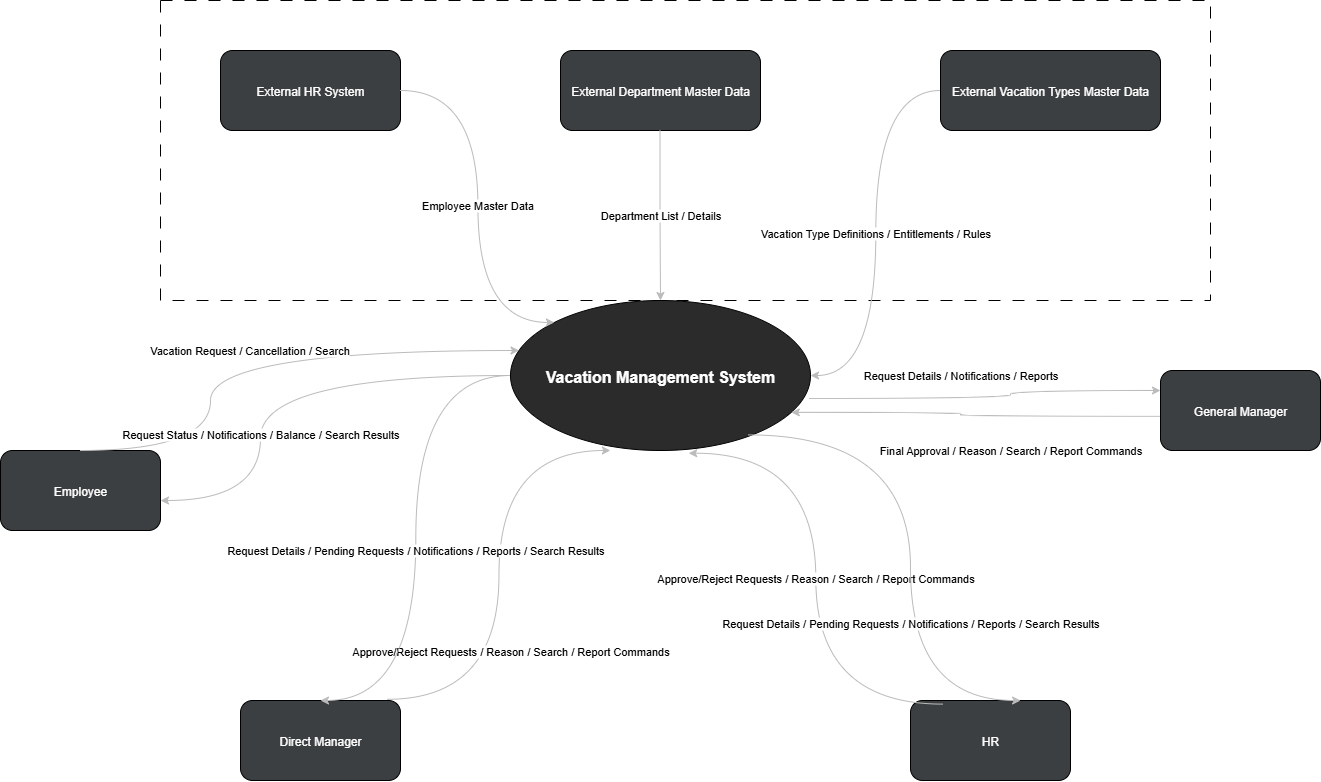
\includegraphics[width=0.8\textwidth]{Diagrams/Context/context.drawio.png}
\caption{System Context Diagram}
\label{fig:context}
\end{figure}

\subsection{Architecture Overview}
The system follows a three-tier architecture:
\begin{itemize}
    \item \textbf{Presentation Tier}: Web and mobile interfaces
    \item \textbf{Business Logic Tier}: Application services and workflows
    \item \textbf{Data Tier}: Database and file storage
\end{itemize}

\subsection{Component Design}
\begin{itemize}
    \item \textbf{User Management Module}: Authentication and authorization
    \item \textbf{Vacation Management Module}: Core business logic
    \item \textbf{Workflow Engine}: Approval process management
    \item \textbf{Reporting Module}: Report generation and export
    \item \textbf{Notification Module}: Communication services
    \item \textbf{Balance Management Module}: Automated vacation balance calculations
\end{itemize}

\subsection{State Management}
The system manages various states for vacation requests and the overall workflow:

\begin{figure}[H]
\centering
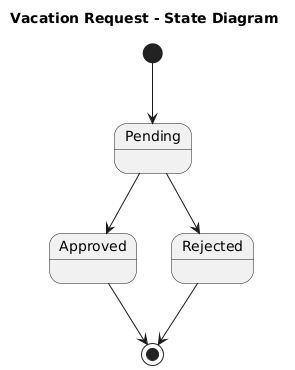
\includegraphics[width=0.6\textwidth]{Diagrams/State-Diagram/State-Diagram.png}
\caption{Vacation Request State Diagram}
\label{fig:state-diagram}
\end{figure}

\subsection{Workflow Processes}
The system implements several key workflow processes:

\subsubsection{Basic Vacation Request Flow}
\begin{figure}[H]
\centering
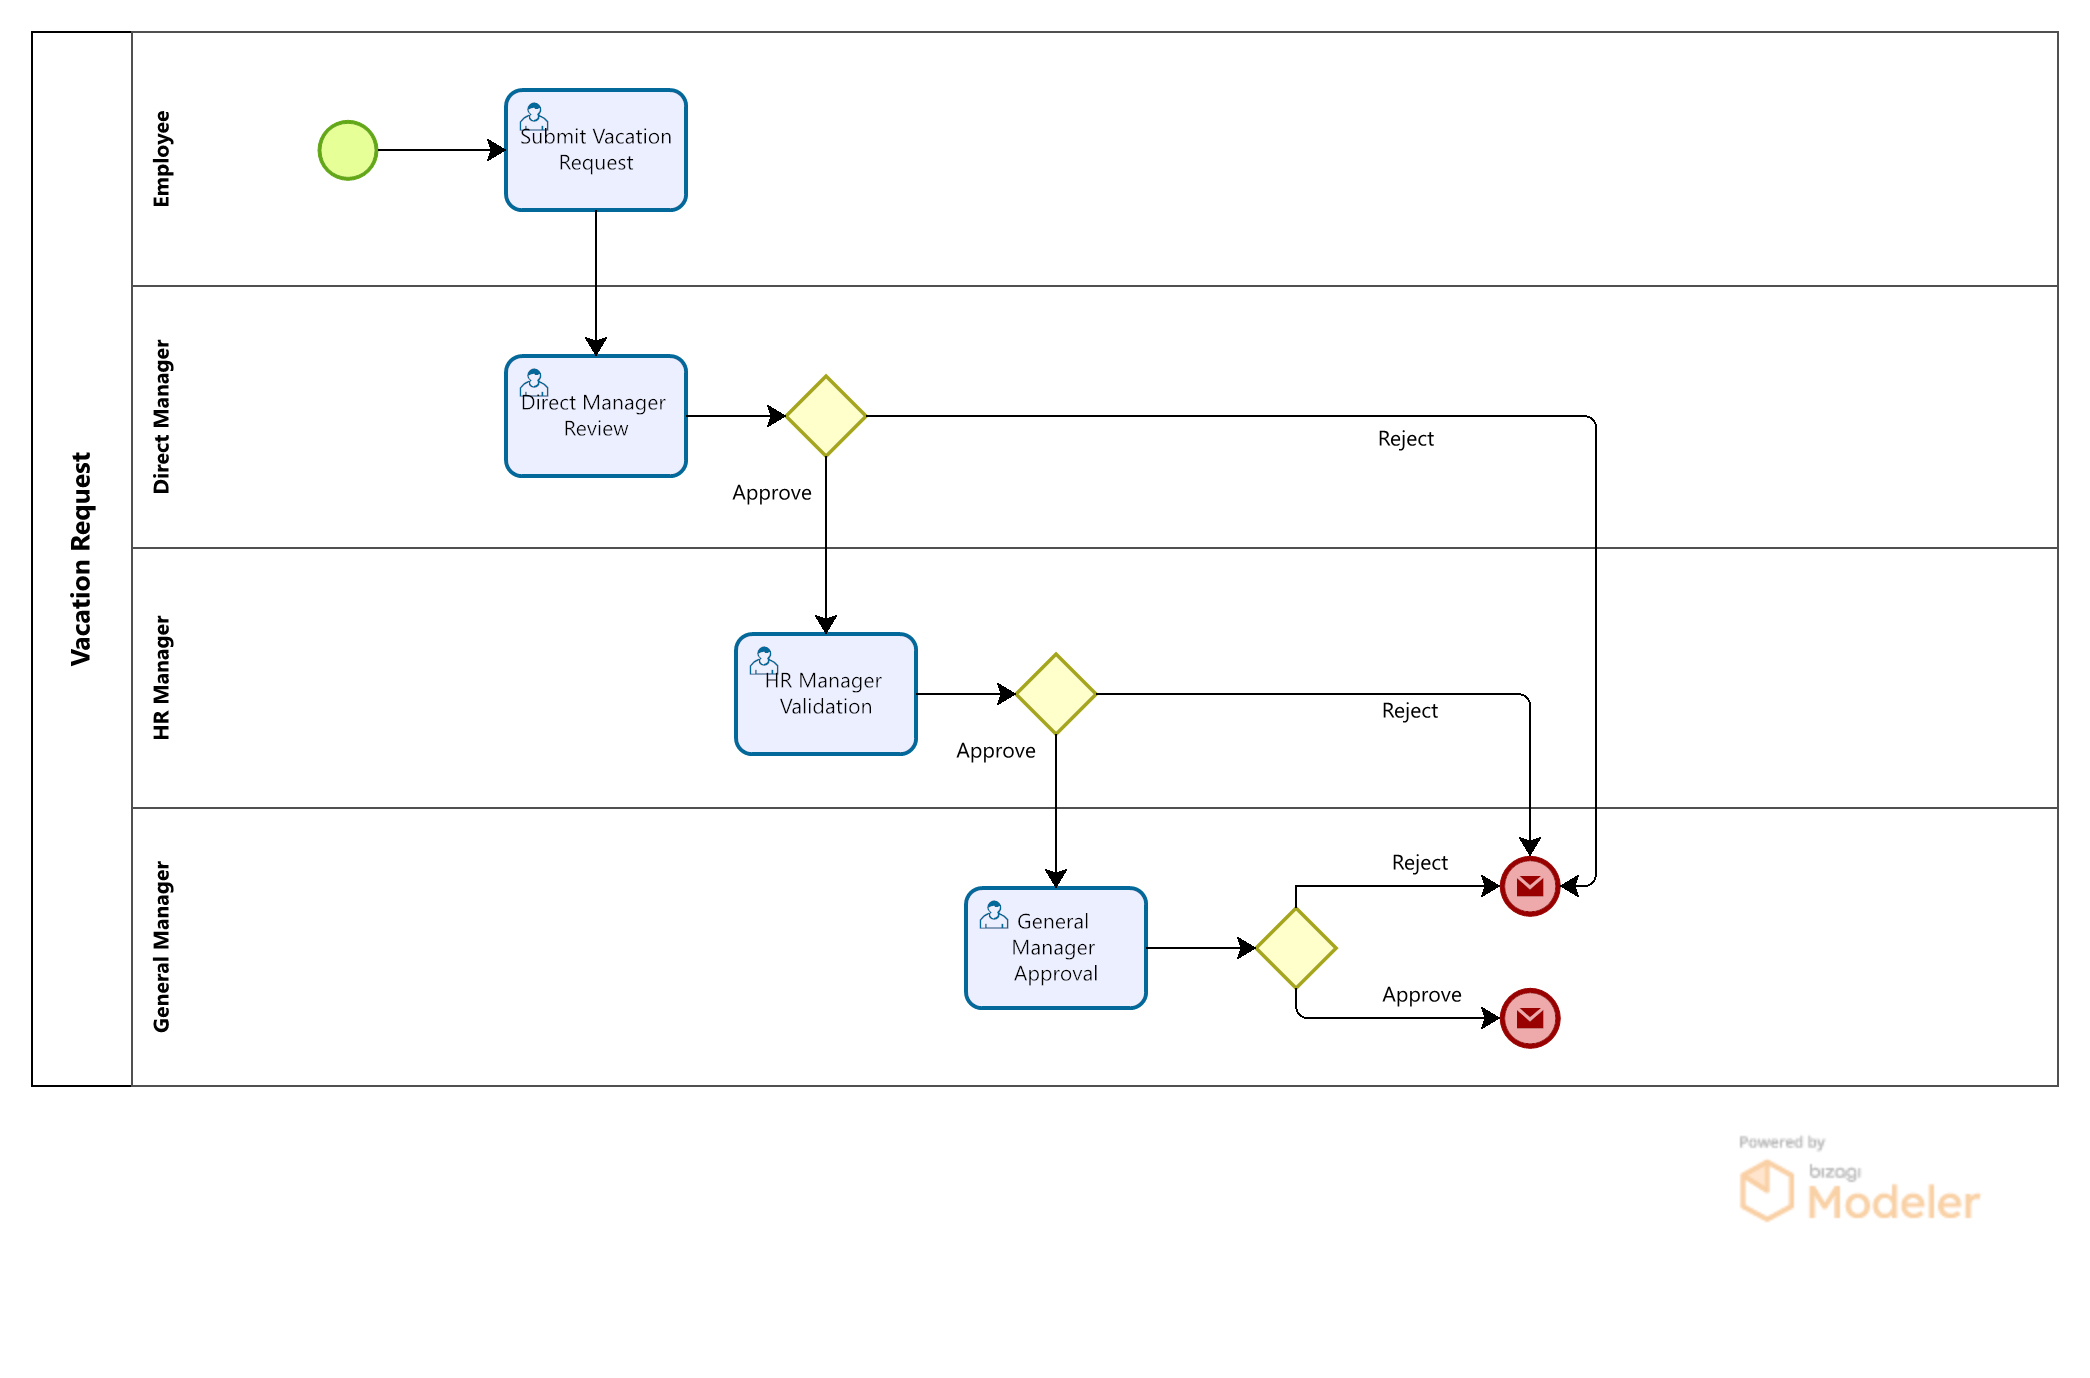
\includegraphics[width=0.8\textwidth]{Diagrams/Workflows/Vacation-Request-Basic-Flow/Vacation-Request-Basic-Flow.png}
\caption{Basic Vacation Request Workflow}
\label{fig:basic-flow}
\end{figure}

\subsubsection{Escalation to Sponsor Flow}
\begin{figure}[H]
\centering
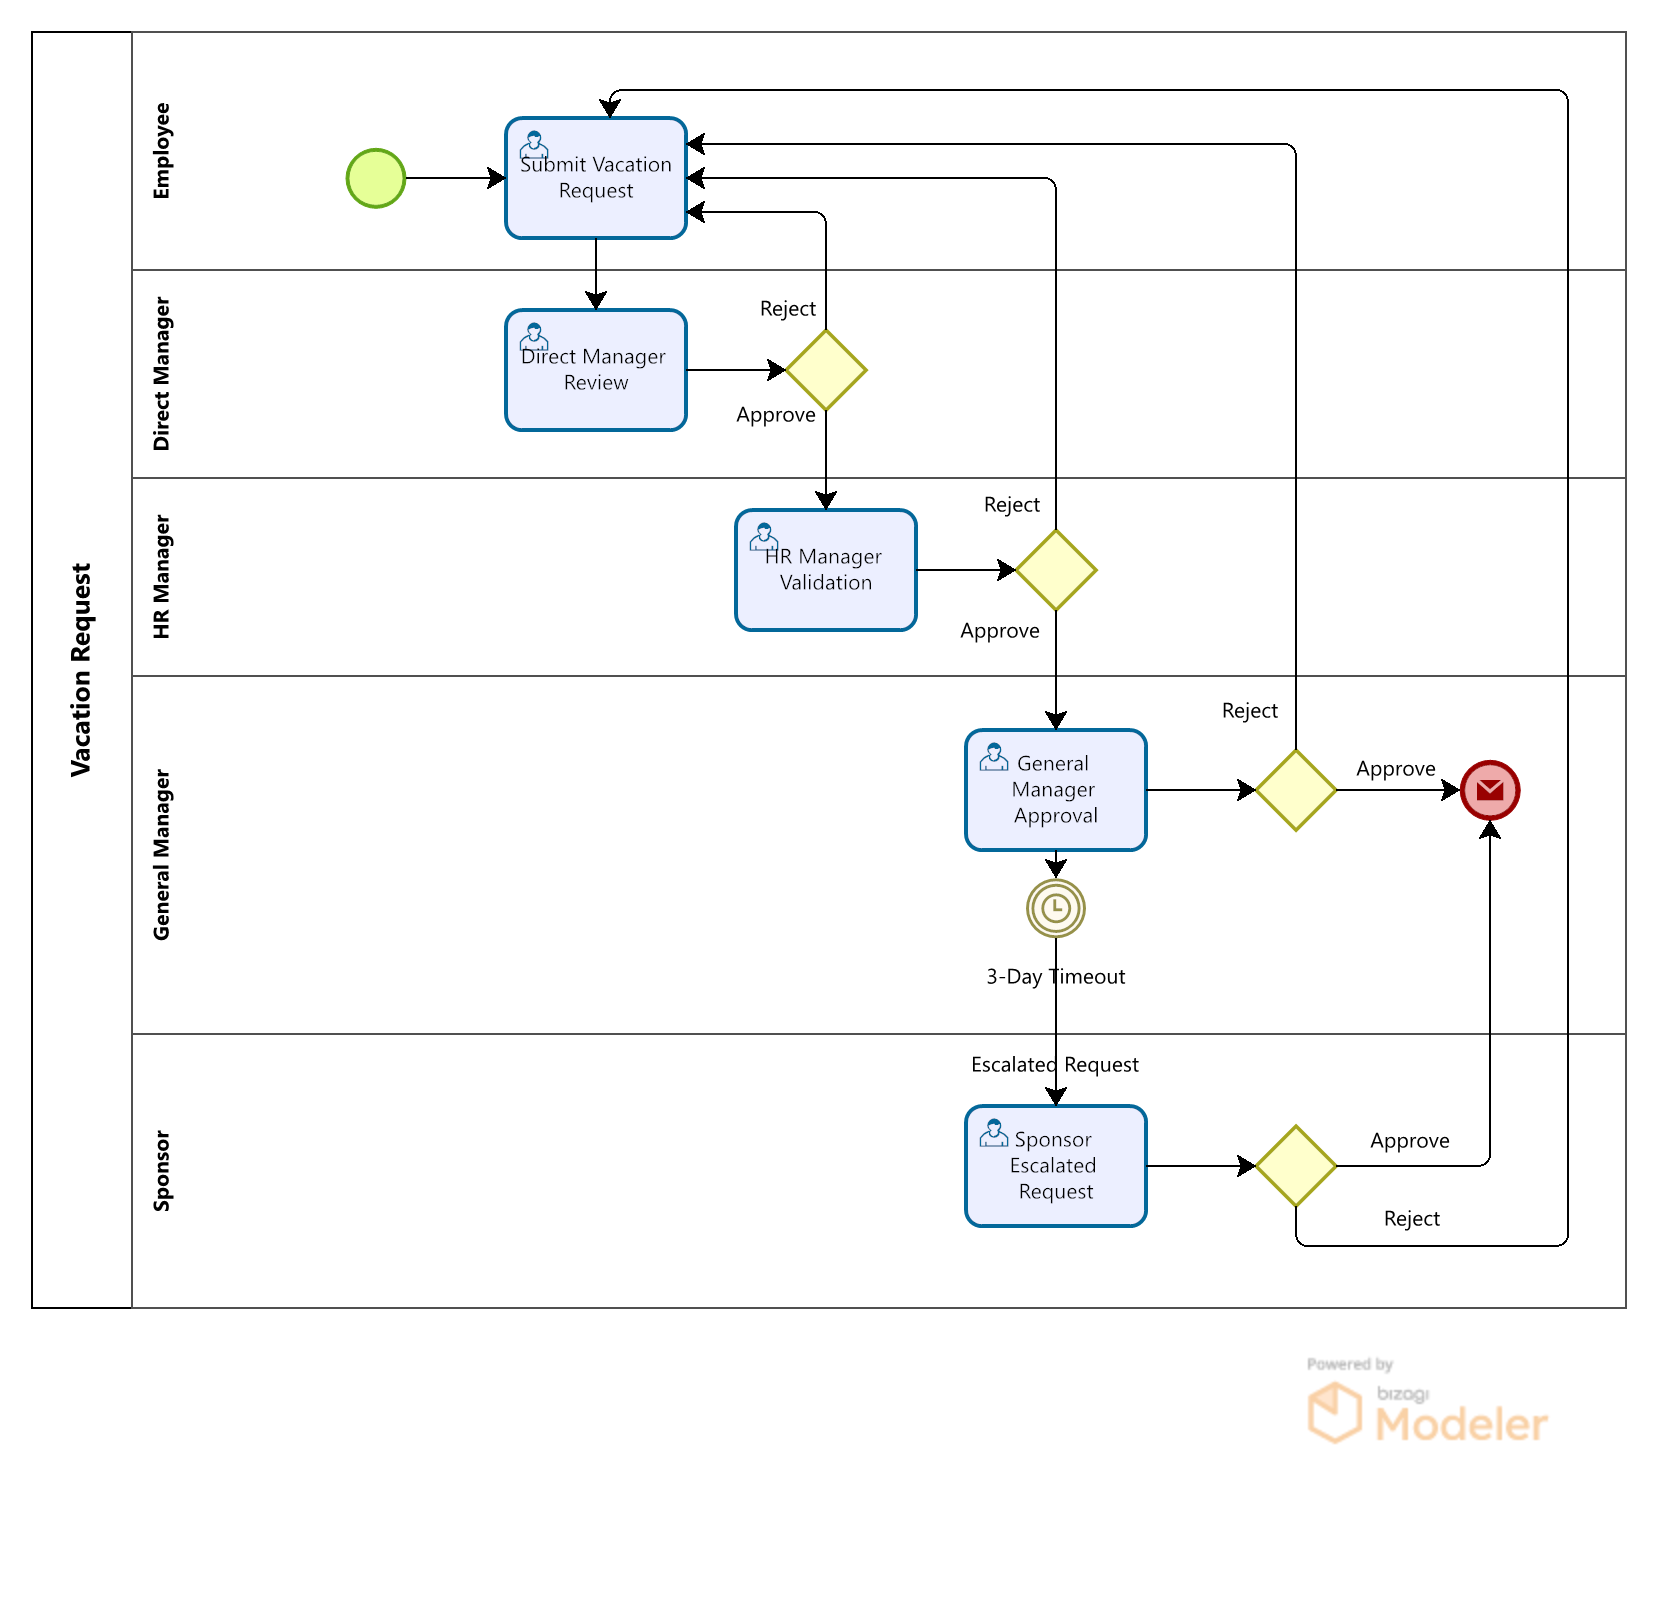
\includegraphics[width=0.8\textwidth]{Diagrams/Workflows/Vacation-Request-Escalation-to-Sponsor/Vacation-Request-Escalation-to-Sponsor.png}
\caption{Vacation Request Escalation to Sponsor Workflow}
\label{fig:escalation-flow}
\end{figure}

\subsubsection{Resubmission After Rejection Flow}
\begin{figure}[H]
\centering
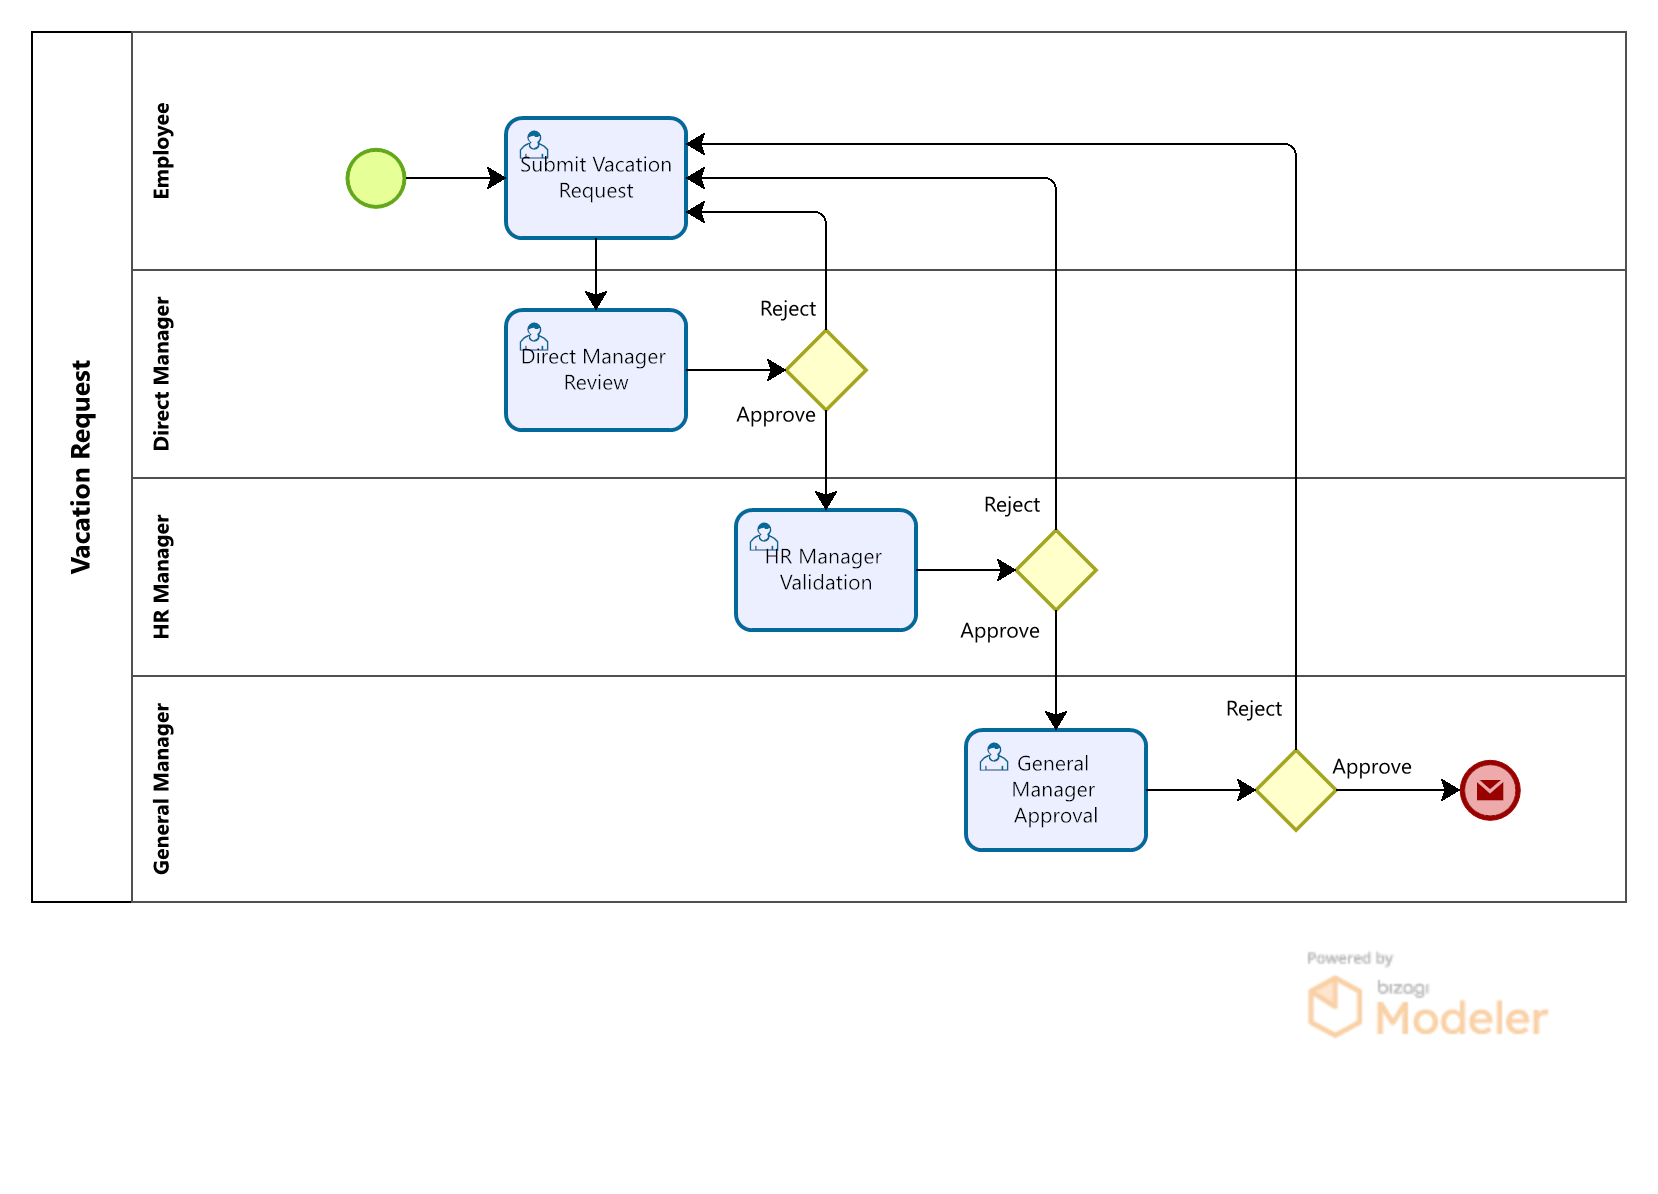
\includegraphics[width=0.8\textwidth]{Diagrams/Workflows/Vacation-Request-Resubmission-After-Rejection/Vacation-Request-Resubmission-After-Rejection.png}
\caption{Vacation Request Resubmission After Rejection Workflow}
\label{fig:resubmission-flow}
\end{figure}

\section{Use Cases and Functional Requirements}

Based on the comprehensive use case analysis in All-UseCases.json, the system implements the following key use cases:

\subsection{UC-1: Employee Submits Vacation Request}
\begin{itemize}
    \item \textbf{Primary Actor}: Employee
    \item \textbf{Goal}: Submit a vacation request for approval
    \item \textbf{Preconditions}: Employee authenticated, has leave balance, is not a trainee
    \item \textbf{Main Flow}: Navigate to form, enter details, submit
    \item \textbf{Postconditions}: Request created with status "Pending Approval", workflow initiated
    \item \textbf{Business Rules}: 
    \begin{itemize}
        \item End date must be after start date
        \item Requested days must not exceed available leave balance
        \item Sick leave requires medical certificate attachment
        \item No overlapping requests for same employee
    \end{itemize}
\end{itemize}

\begin{figure}[H]
\centering
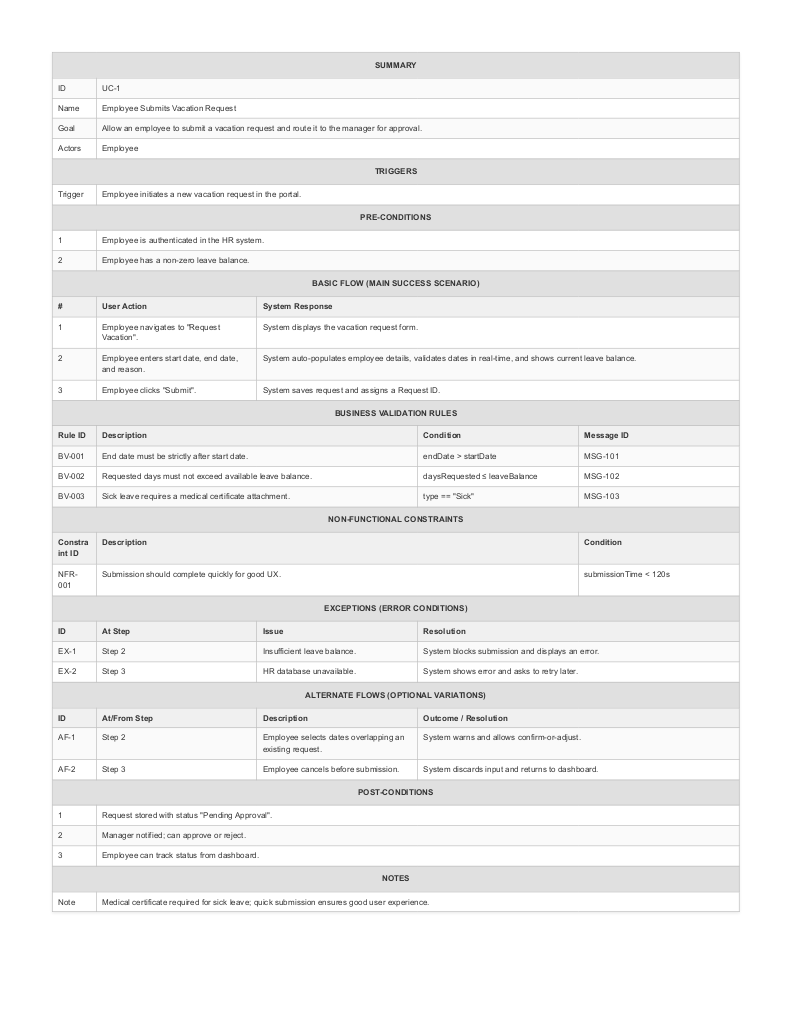
\includegraphics[width=0.8\textwidth]{Use-Cases/UC-1-Employee-Vacation-Request/UC-1-Employee-Vacation-Request-1.png}
\caption{UC-1: Employee Vacation Request Use Case}
\label{fig:uc1}
\end{figure}

\subsection{UC-2: Employee Submits Vacation Cancellation Request}
\begin{itemize}
    \item \textbf{Primary Actor}: Employee
    \item \textbf{Goal}: Cancel a pending or approved vacation request before its start date
    \item \textbf{Preconditions}: Request exists in Pending or Approved status, vacation has not started
    \item \textbf{Main Flow}: Select request, provide cancellation reason, submit
    \item \textbf{Postconditions}: Cancellation request created with status "Pending"
    \item \textbf{Business Rules}: Only requests in Pending or Approved status can be cancelled
\end{itemize}

\begin{figure}[H]
\centering
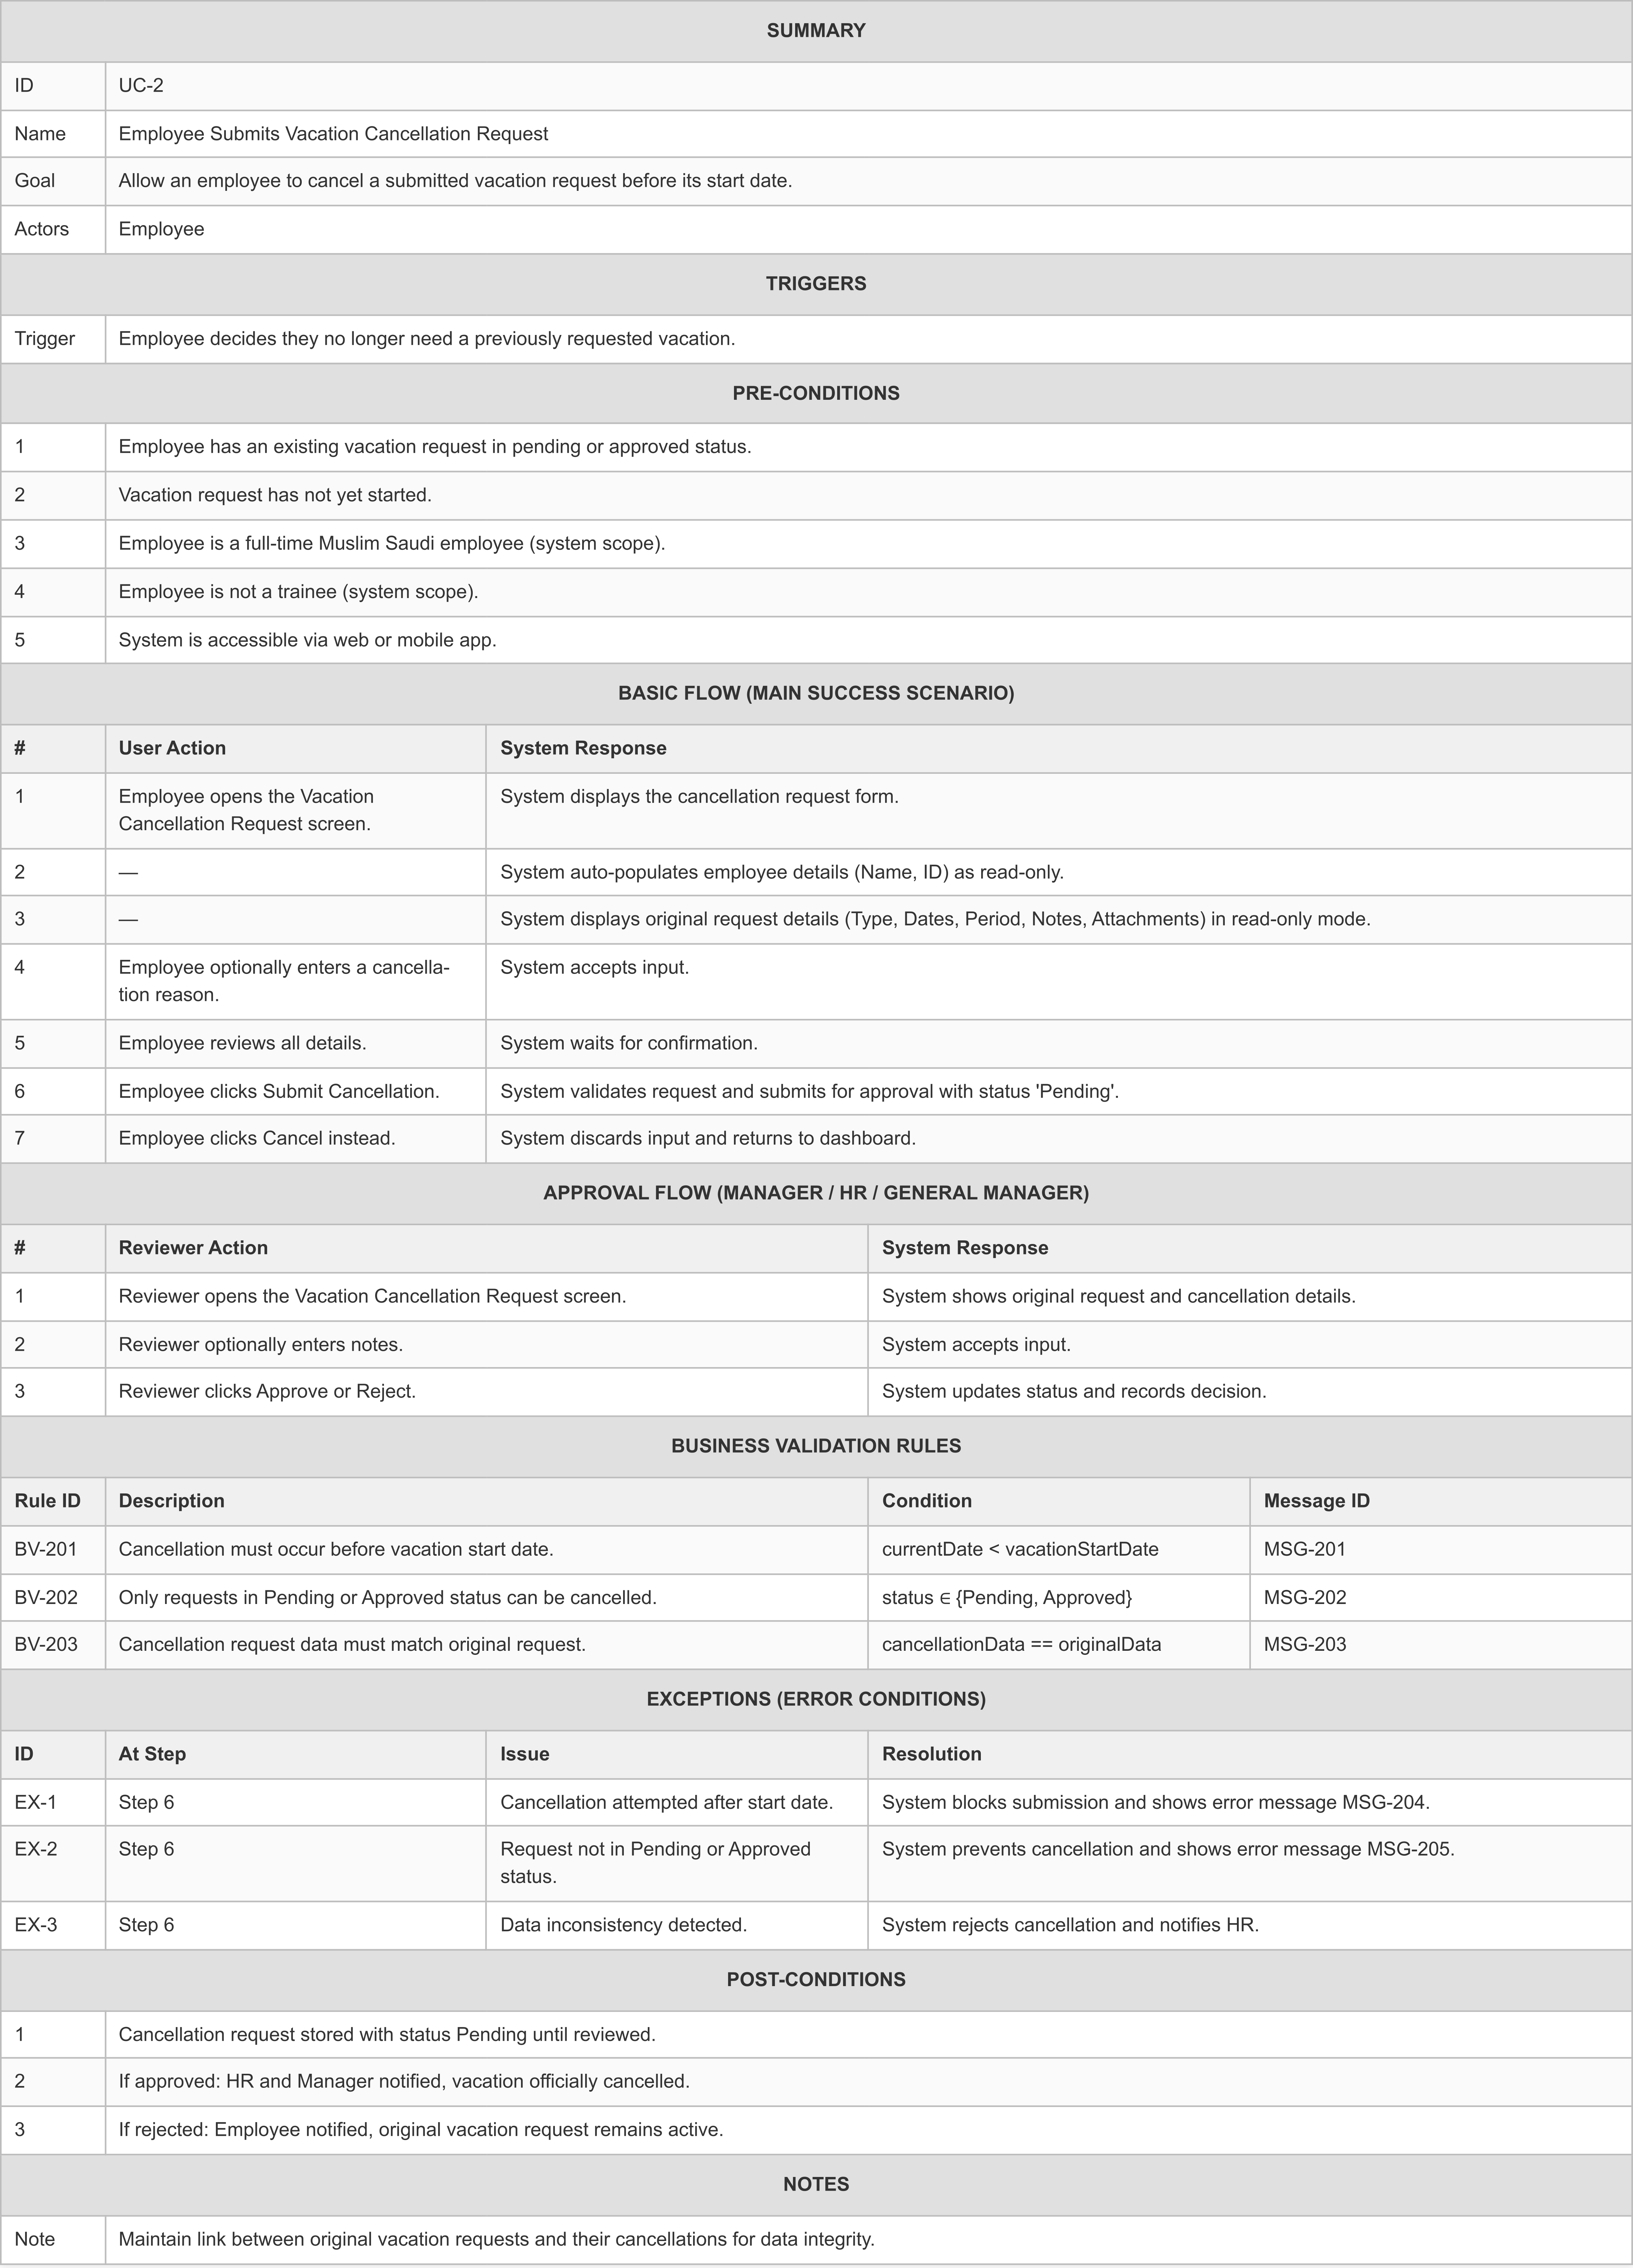
\includegraphics[width=0.8\textwidth]{Use-Cases/UC-2-Employee-Vacation-Cancellation-Request/UC-2-Employee-Vacation-Cancellation-Request-1.png}
\caption{UC-2: Employee Vacation Cancellation Request Use Case}
\label{fig:uc2}
\end{figure}

\subsection{UC-3: My Vacation Requests}
\begin{itemize}
    \item \textbf{Primary Actor}: Employee
    \item \textbf{Goal}: View and manage personal vacation requests
    \item \textbf{Preconditions}: Employee has access to the system
    \item \textbf{Main Flow}: Navigate to dashboard, view summary, expand details
    \item \textbf{Postconditions}: Employee has visibility into all requests with detailed view
    \item \textbf{Business Rules}: Cancel button only enabled when rules allow
\end{itemize}

\begin{figure}[H]
\centering
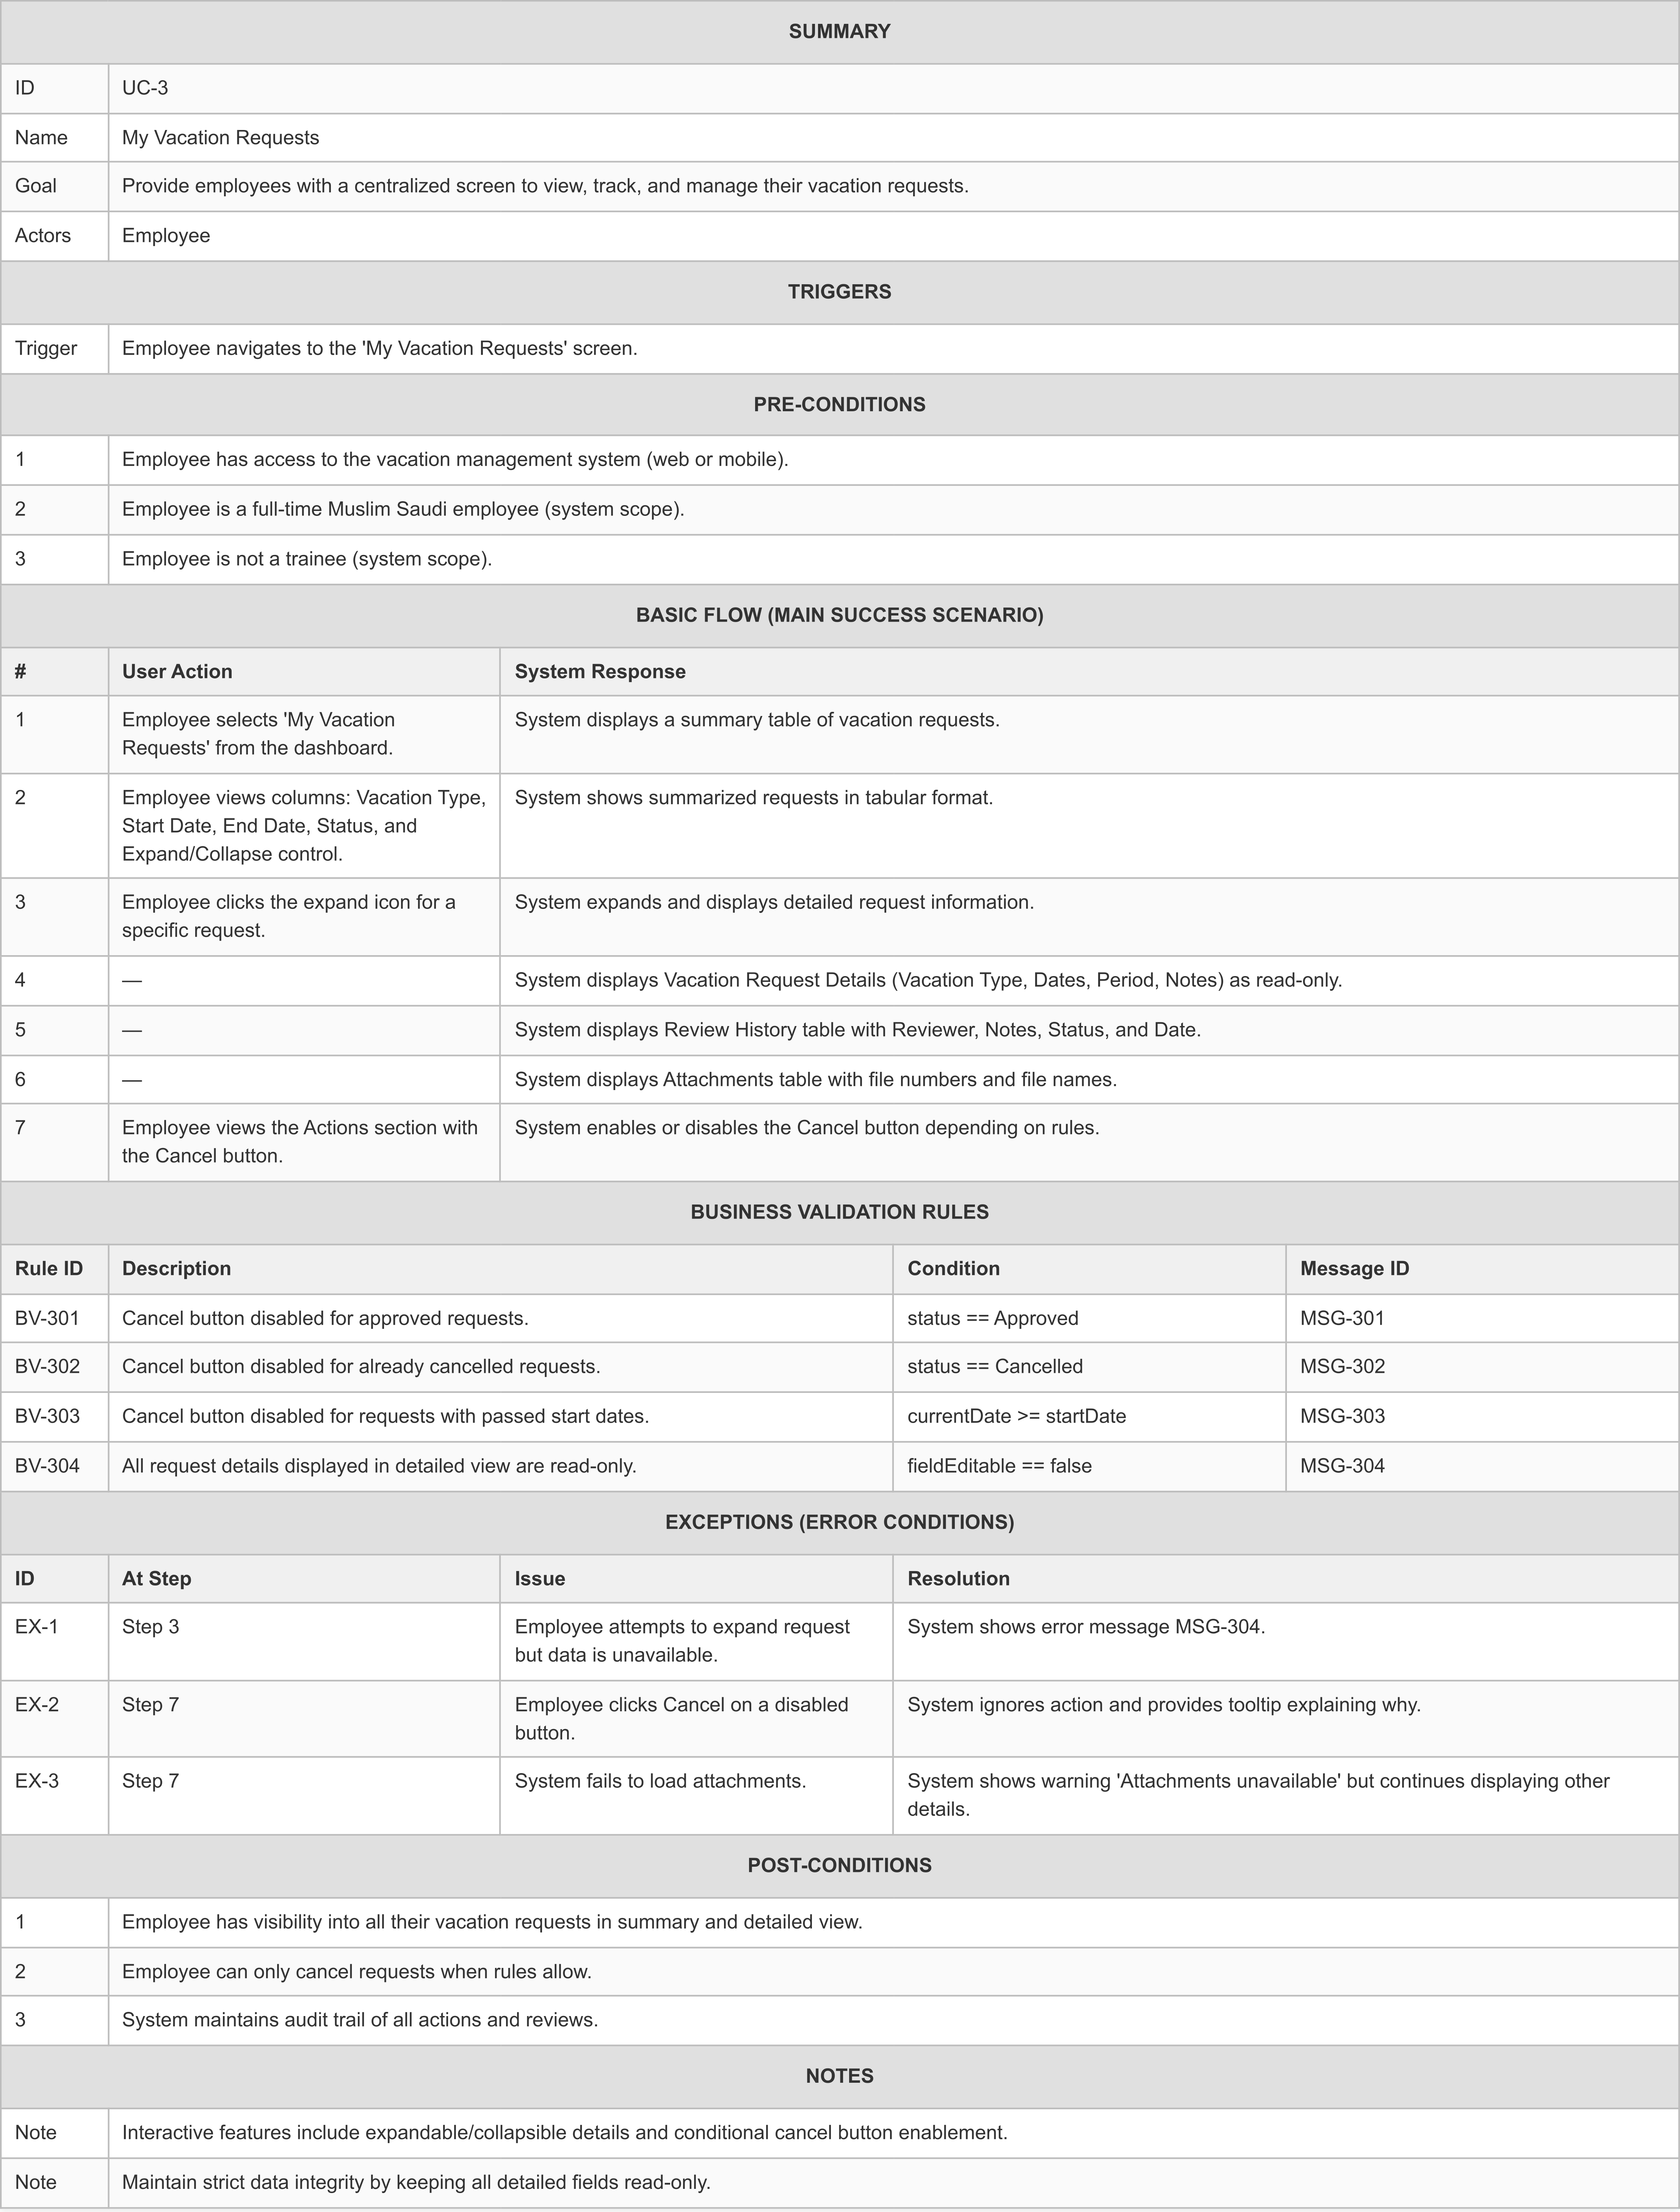
\includegraphics[width=0.8\textwidth]{Use-Cases/UC-3-My-Vacation-Requests/UC-3-My-Vacation-Requests-1.png}
\caption{UC-3: My Vacation Requests Use Case}
\label{fig:uc3}
\end{figure}

\subsection{UC-4: Review Vacation Request (Approval/Rejection)}
\begin{itemize}
    \item \textbf{Primary Actor}: Direct Manager, HR, General Manager
    \item \textbf{Goal}: Review, approve, or reject employee vacation requests
    \item \textbf{Preconditions}: Valid vacation request exists for review
    \item \textbf{Main Flow}: View request details, make decision, provide reason
    \item \textbf{Postconditions}: Request status updated, notifications sent
    \item \textbf{Business Rules}: Reason for decision is mandatory for all reviewers
\end{itemize}

\begin{figure}[H]
\centering
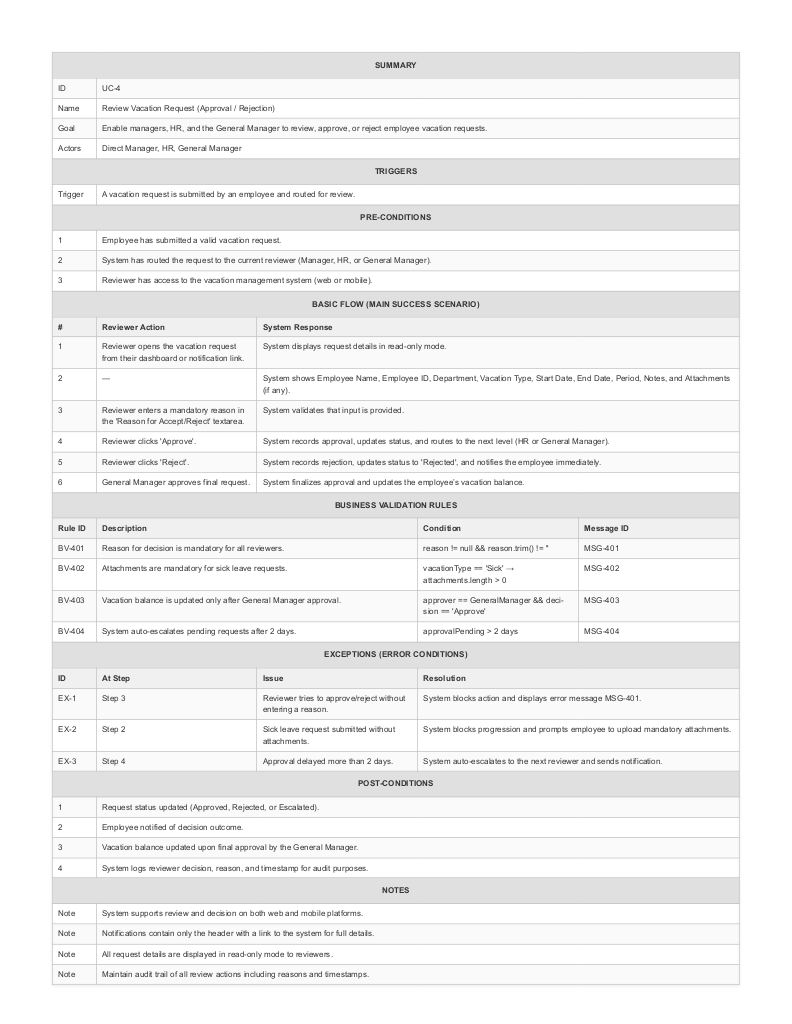
\includegraphics[width=0.8\textwidth]{Use-Cases/UC-4-Review-Vacation-Request/UC-4-Review-Vacation-Request-1.png}
\caption{UC-4: Review Vacation Request Use Case}
\label{fig:uc4}
\end{figure}

\subsection{UC-5: Review Vacation Cancellation Request}
\begin{itemize}
    \item \textbf{Primary Actor}: Manager, HR
    \item \textbf{Goal}: Review and approve/reject vacation cancellation requests
    \item \textbf{Preconditions}: Valid cancellation request exists
    \item \textbf{Main Flow}: View original and cancellation details, make decision
    \item \textbf{Postconditions}: Cancellation status updated, notifications sent
    \item \textbf{Business Rules}: Cancellation must occur before vacation start date
\end{itemize}

\begin{figure}[H]
\centering
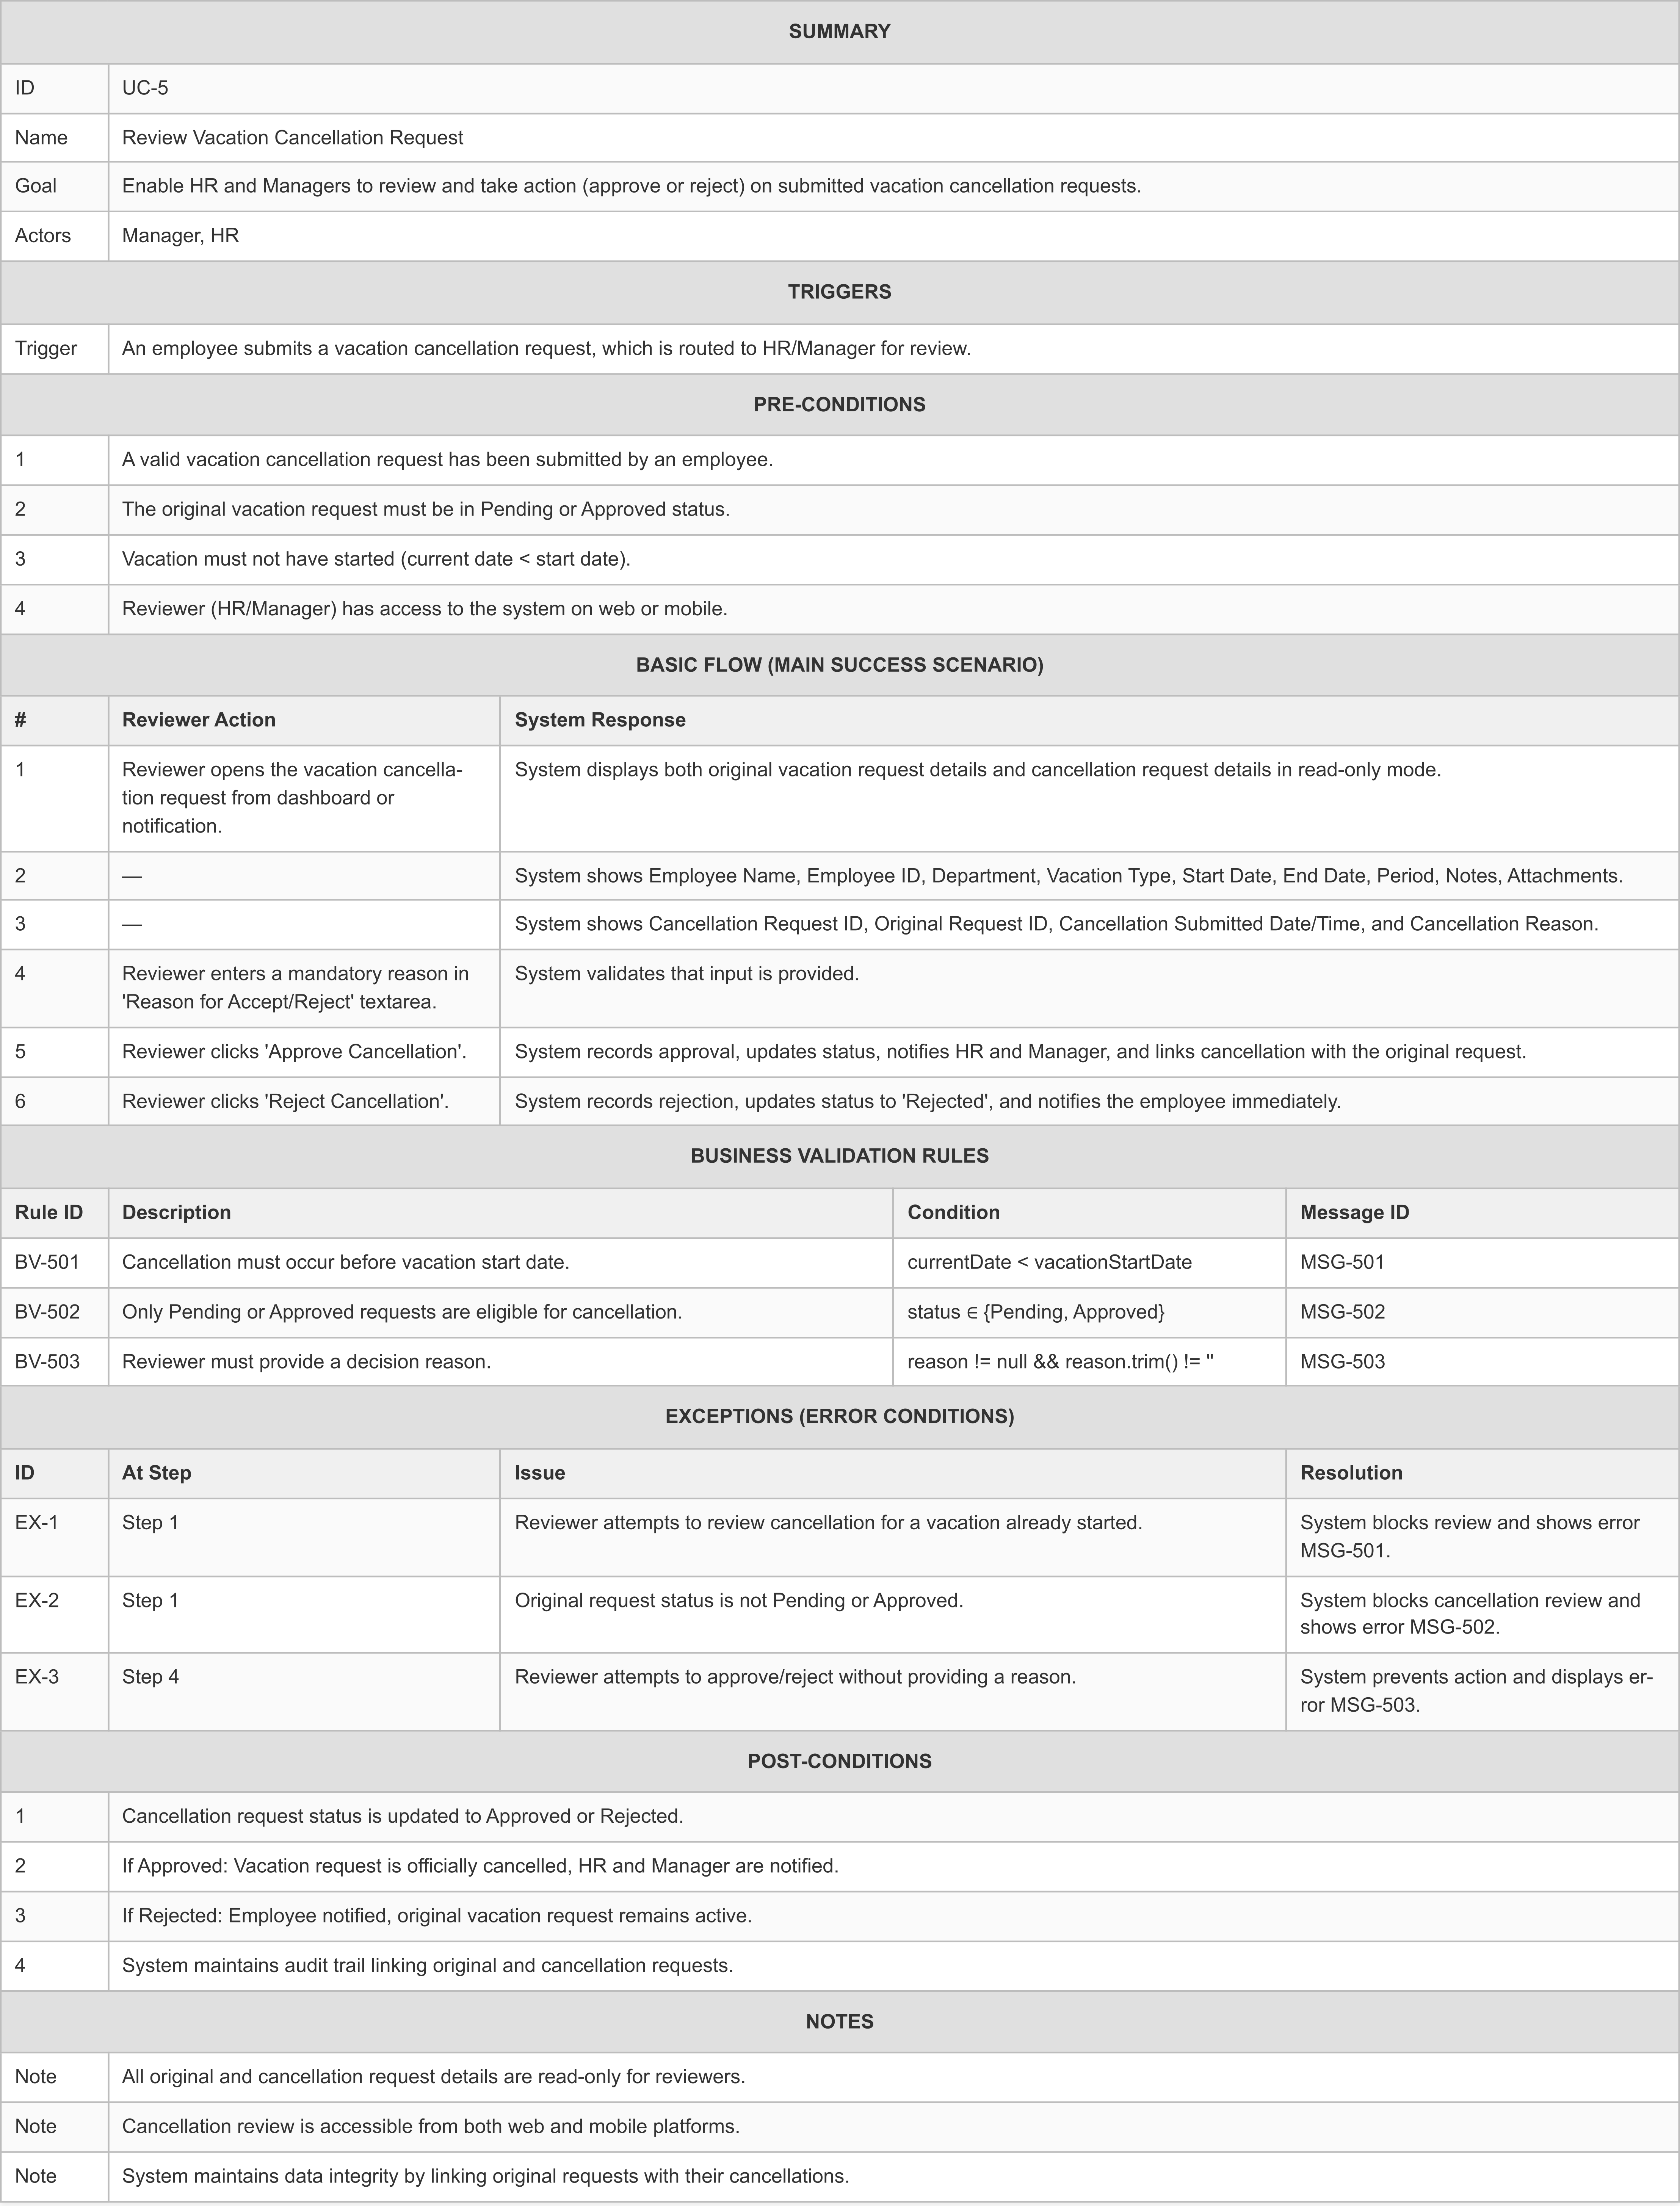
\includegraphics[width=0.8\textwidth]{Use-Cases/UC-5-Review-Vacation-Cancellation-Request/UC-5-Review-Vacation-Cancellation-Request-1.png}
\caption{UC-5: Review Vacation Cancellation Request Use Case}
\label{fig:uc5}
\end{figure}

\subsection{UC-6: Pending Vacation Requests}
\begin{itemize}
    \item \textbf{Primary Actor}: Manager, HR
    \item \textbf{Goal}: View and manage all pending vacation requests
    \item \textbf{Preconditions}: Pending requests exist, user has access rights
    \item \textbf{Main Flow}: View grid of pending requests, navigate to detailed review
    \item \textbf{Postconditions}: Reviewer can access detailed review for any pending request
    \item \textbf{Business Rules}: Only pending requests appear on this screen
\end{itemize}

\begin{figure}[H]
\centering
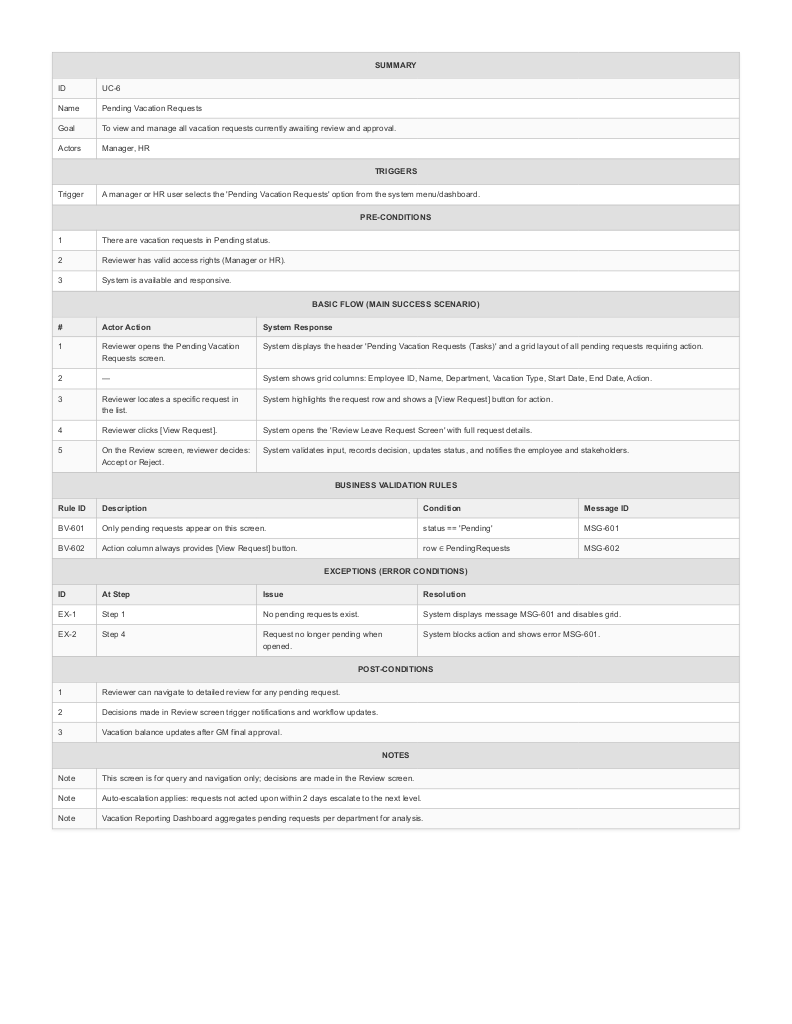
\includegraphics[width=0.8\textwidth]{Use-Cases/UC-6-Pending-Vacation-Requests/UC-6-Pending-Vacation-Requests-1.png}
\caption{UC-6: Pending Vacation Requests Use Case}
\label{fig:uc6}
\end{figure}

\subsection{UC-7: Vacation Inquiry (Search Parameters)}
\begin{itemize}
    \item \textbf{Primary Actor}: HR, Managers, Authorized Employees
    \item \textbf{Goal}: Input search criteria for vacation inquiries
    \item \textbf{Preconditions}: User has valid system access
    \item \textbf{Main Flow}: Select filters, generate report
    \item \textbf{Postconditions}: Search results displayed or validation errors shown
    \item \textbf{Business Rules}: All search parameters are optional
\end{itemize}

\begin{figure}[H]
\centering
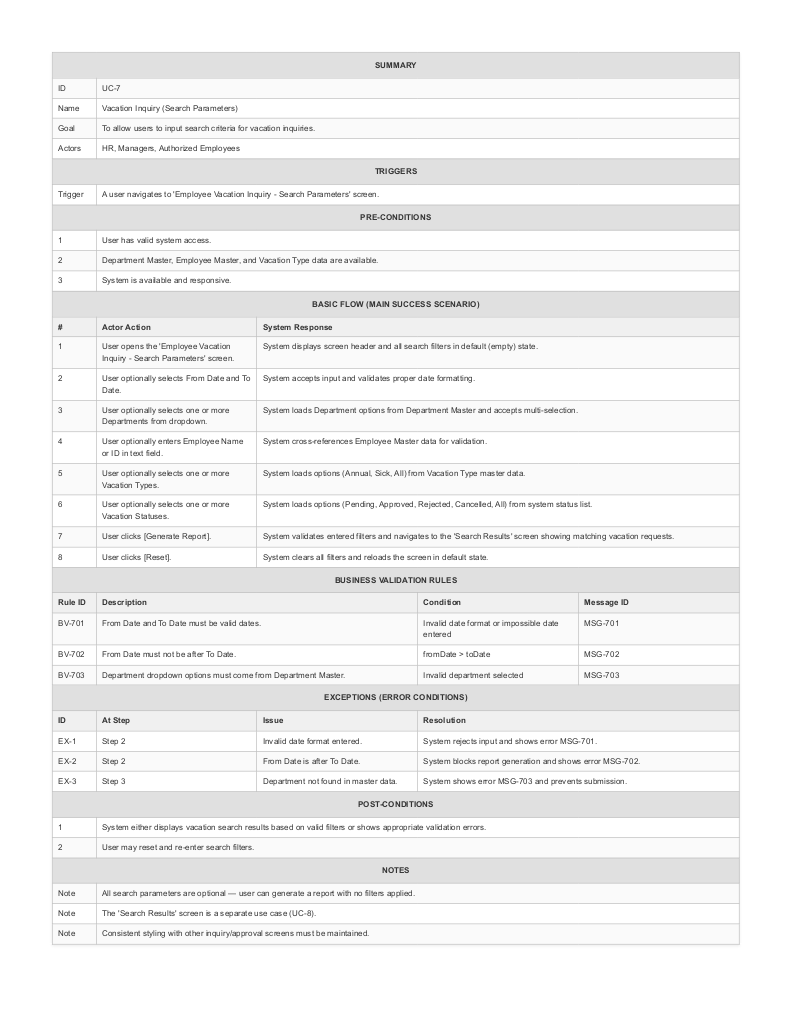
\includegraphics[width=0.8\textwidth]{Use-Cases/UC-7-Vacation-Inquiry-Search-Parameters/UC-7-Vacation-Inquiry-Search-Parameters-1.png}
\caption{UC-7: Vacation Inquiry Search Parameters Use Case}
\label{fig:uc7}
\end{figure}

\subsection{UC-8: Vacation Inquiry (Search Results)}
\begin{itemize}
    \item \textbf{Primary Actor}: HR, Managers, Authorized Employees
    \item \textbf{Goal}: Display inquiry results and provide action options
    \item \textbf{Preconditions}: Valid search criteria executed from UC-7
    \item \textbf{Main Flow}: View results grid, perform actions (print, export, pagination)
    \item \textbf{Postconditions}: User can interact with results and perform actions
    \item \textbf{Business Rules}: Print option only available for approved requests
\end{itemize}

\begin{figure}[H]
\centering
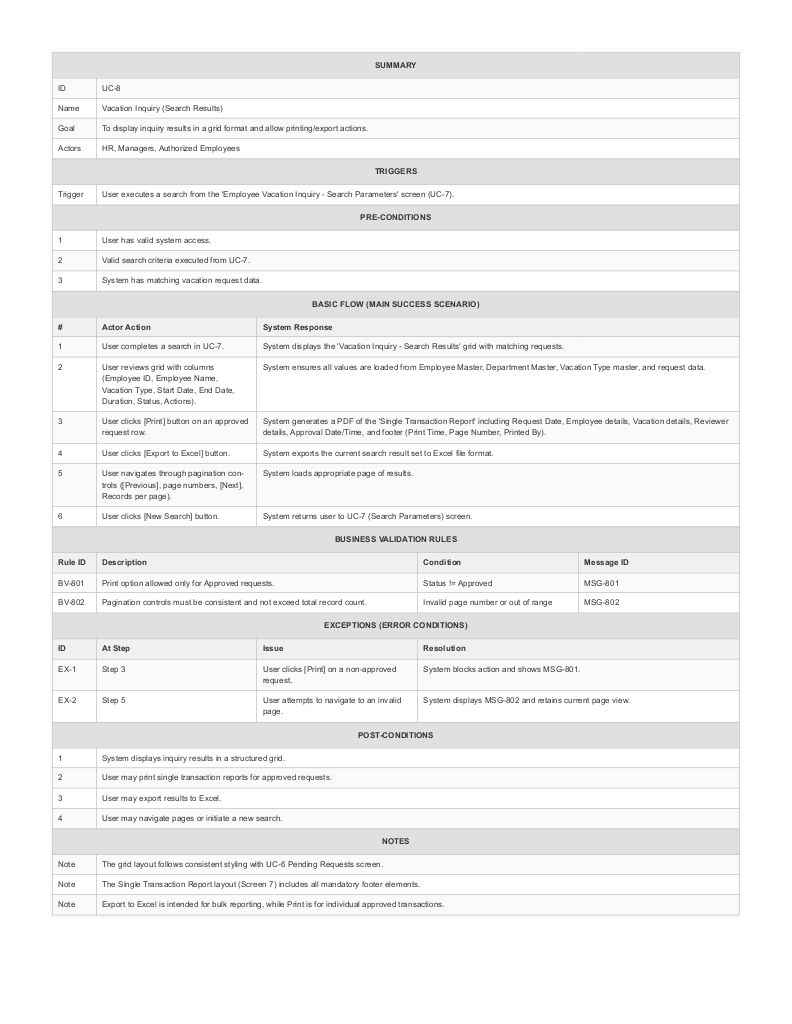
\includegraphics[width=0.8\textwidth]{Use-Cases/UC-8-Vacation-Inquiry-Search-Results/UC-8-Vacation-Inquiry-Search-Results-1.png}
\caption{UC-8: Vacation Inquiry Search Results Use Case}
\label{fig:uc8}
\end{figure}

\subsection{UC-9: Print Single Vacation Transaction Report (PDF)}
\begin{itemize}
    \item \textbf{Primary Actor}: HR, Managers, Authorized Employees
    \item \textbf{Goal}: Generate PDF for individual approved vacation request
    \item \textbf{Preconditions}: Vacation request status must be Approved
    \item \textbf{Main Flow}: Click print button, wait for PDF generation
    \item \textbf{Postconditions}: PDF report generated with complete details
    \item \textbf{Business Rules}: Report can only be generated for approved requests
\end{itemize}

\begin{figure}[H]
\centering
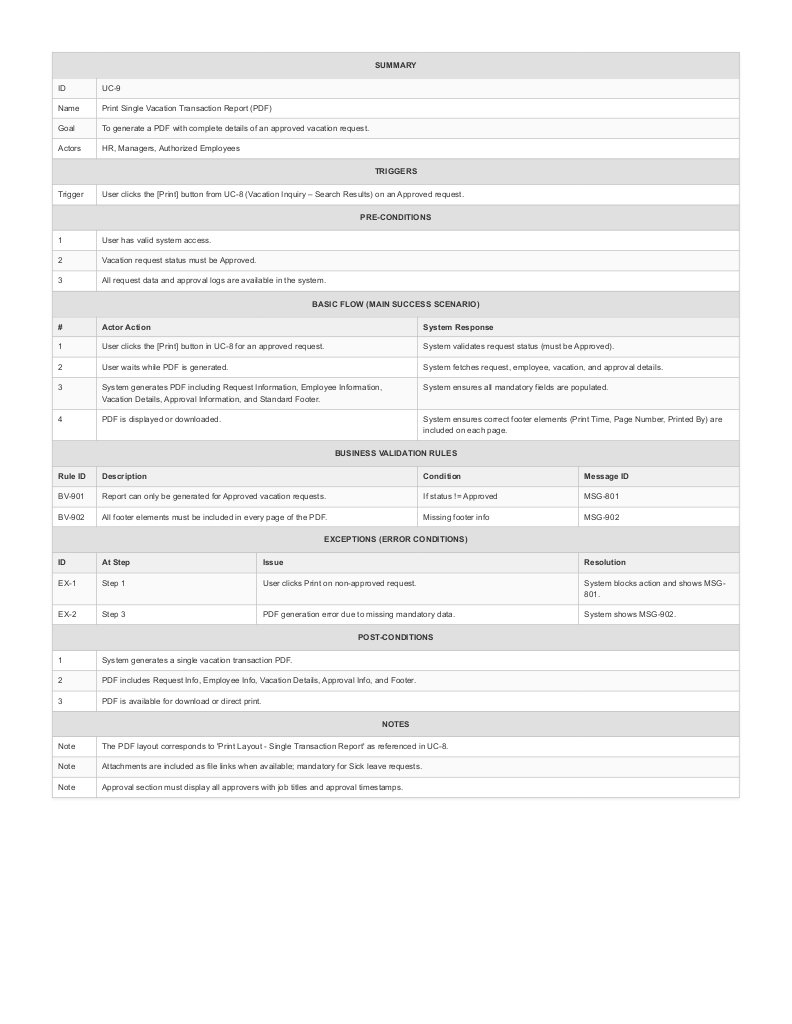
\includegraphics[width=0.8\textwidth]{Use-Cases/UC-9-Print-Single-Vacation-Transaction-Report/UC-9-Print-Single-Vacation-Transaction-Report-1.png}
\caption{UC-9: Print Single Vacation Transaction Report Use Case}
\label{fig:uc9}
\end{figure}

\subsection{UC-10: Print Comparative Annual Report (PDF)}
\begin{itemize}
    \item \textbf{Primary Actor}: HR, Managers, General Management
    \item \textbf{Goal}: Generate annual comparative vacation report by department
    \item \textbf{Preconditions}: User has access to reporting functionality
    \item \textbf{Main Flow}: Select parameters, generate report
    \item \textbf{Postconditions}: Comparative report PDF generated
    \item \textbf{Business Rules}: At least one department must be selected
\end{itemize}

\begin{figure}[H]
\centering
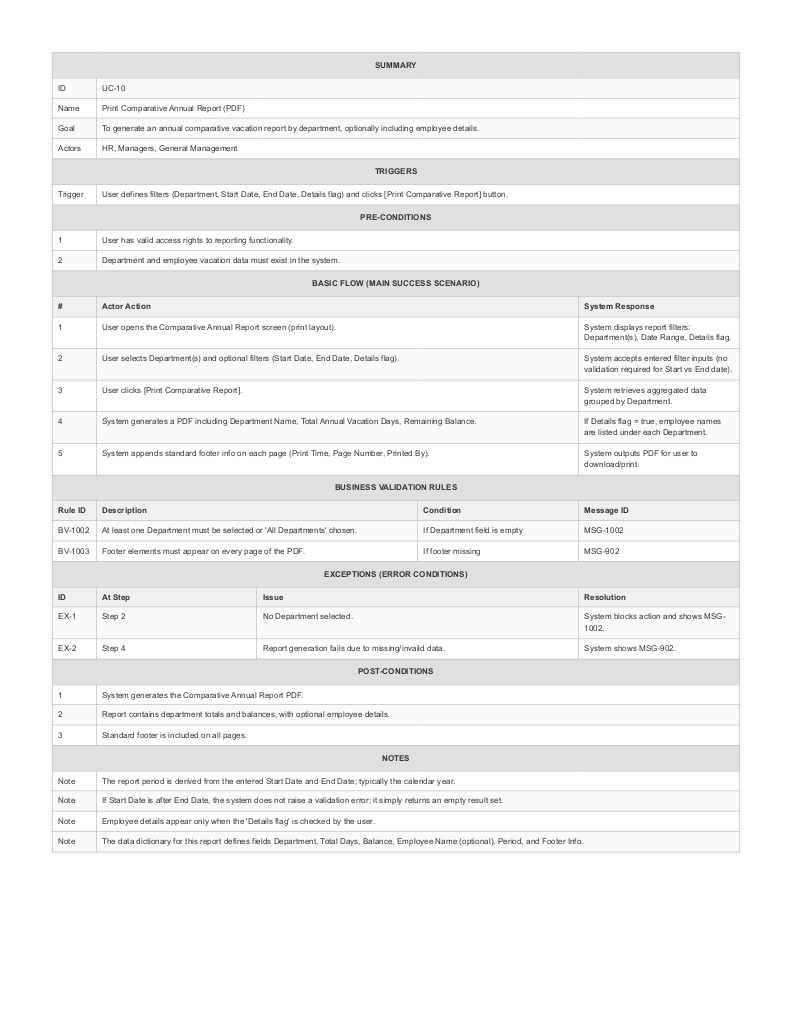
\includegraphics[width=0.8\textwidth]{Use-Cases/UC-10-Print-Comparative-Annual-Report/UC-10-Print-Comparative-Annual-Report-1.png}
\caption{UC-10: Print Comparative Annual Report Use Case}
\label{fig:uc10}
\end{figure}

\subsection{UC-11: Notifications Center}
\begin{itemize}
    \item \textbf{Primary Actor}: Employees, Managers, HR, General Management
    \item \textbf{Goal}: Inform users of vacation-related events and provide quick access
    \item \textbf{Preconditions}: User has valid system access
    \item \textbf{Main Flow}: View notifications, click action buttons
    \item \textbf{Postconditions}: User informed and can navigate to related screens
    \item \textbf{Business Rules}: Notifications appear in reverse chronological order
\end{itemize}

\begin{figure}[H]
\centering
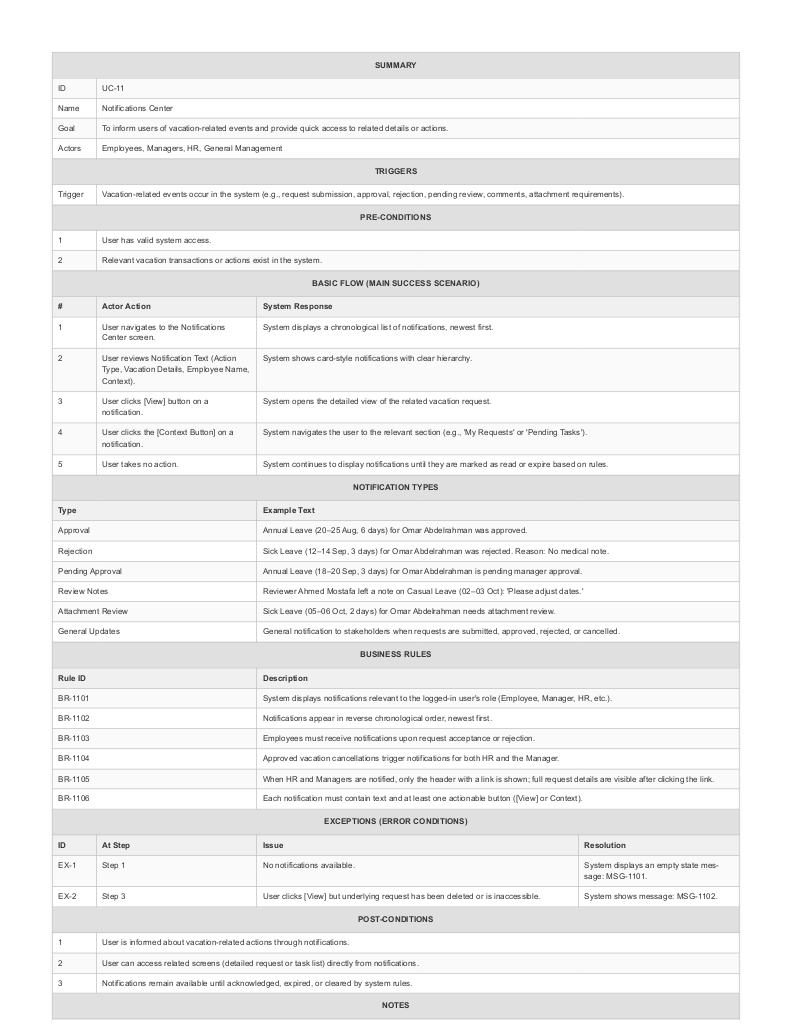
\includegraphics[width=0.8\textwidth]{Use-Cases/UC-11-Notifications-Center/UC-11-Notifications-Center-1.png}
\caption{UC-11: Notifications Center Use Case}
\label{fig:uc11}
\end{figure}

\subsection{UC-12: Automated Update of Employee Annual Vacation Balance}
\begin{itemize}
    \item \textbf{Primary Actor}: System (primary), Employee (view-only), General Manager (approval trigger)
    \item \textbf{Goal}: Automatically manage and update employee vacation balances
    \item \textbf{Preconditions}: Employee is eligible, vacation request approved by GM
    \item \textbf{Main Flow}: System recalculates balance after GM approval
    \item \textbf{Postconditions}: Vacation balances always up-to-date and auto-calculated
    \item \textbf{Business Rules}: No manual overrides permitted, system-only updates
\end{itemize}

\begin{figure}[H]
\centering
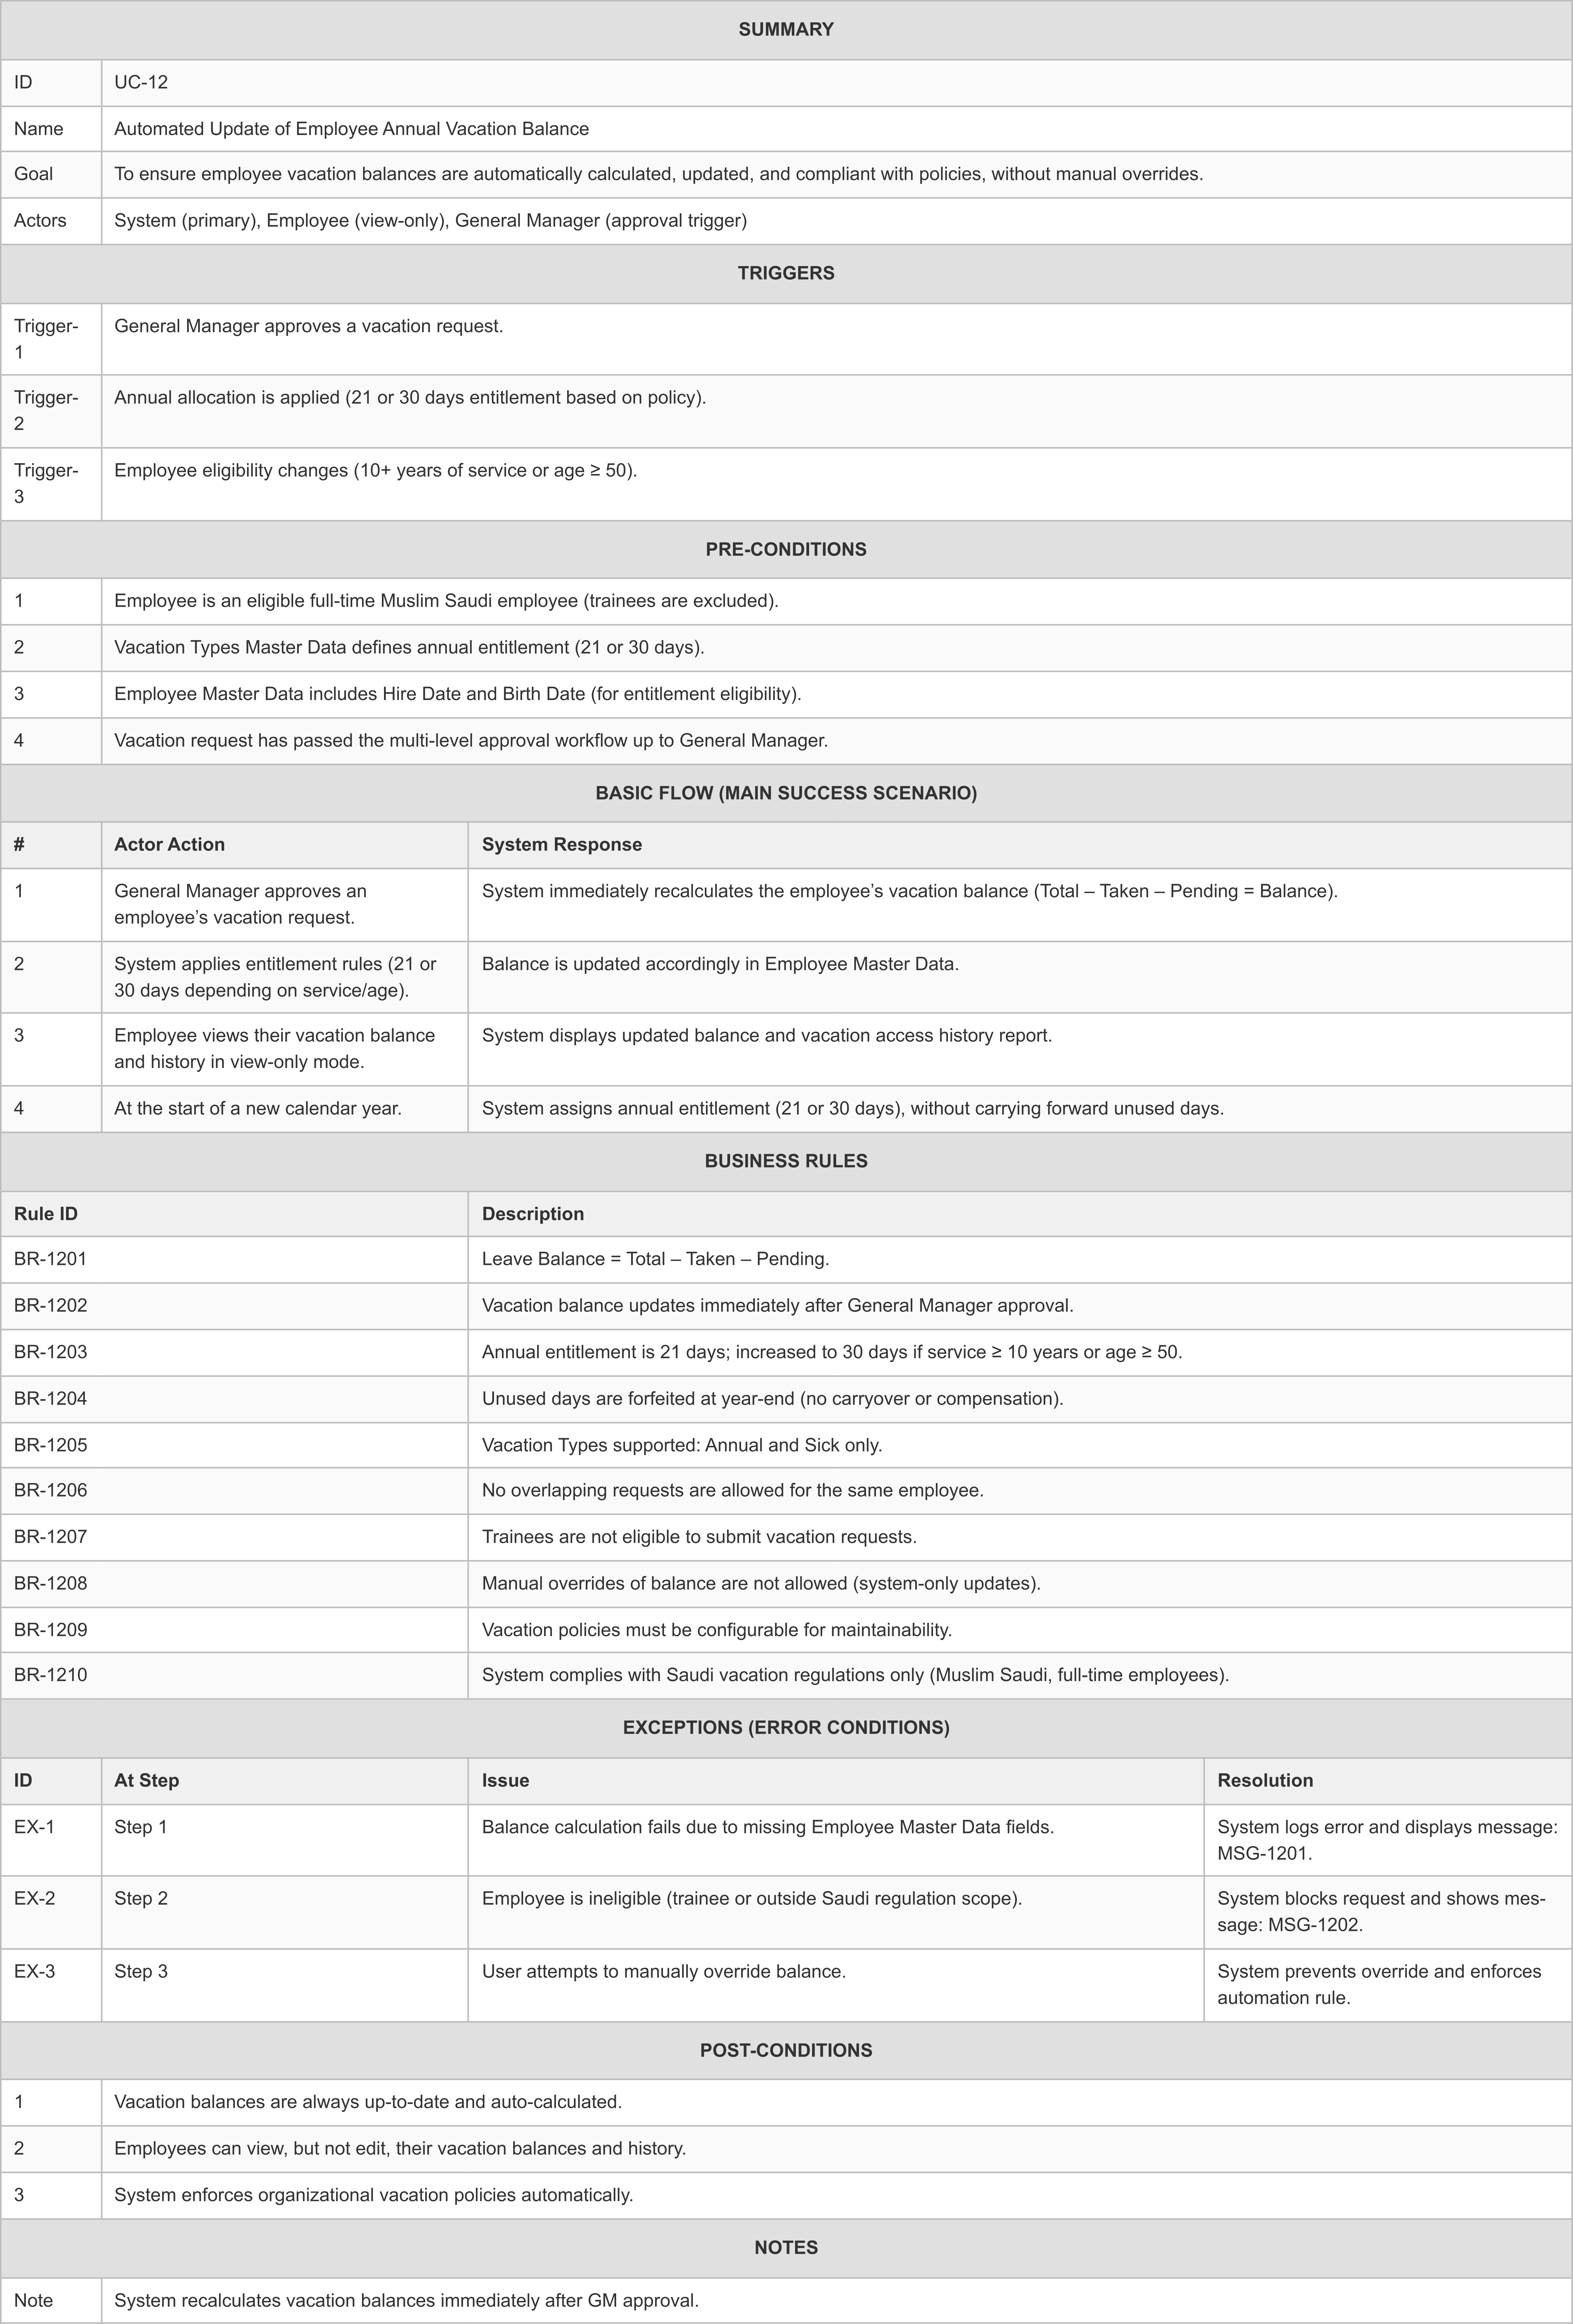
\includegraphics[width=0.8\textwidth]{Use-Cases/UC-12-Automated-Update-of-Employee-Annual-Vacation-Balance/UC-12-Automated-Update-of-Employee-Annual-Vacation-Balance-1.png}
\caption{UC-12: Automated Update of Employee Annual Vacation Balance Use Case}
\label{fig:uc12}
\end{figure}

\section{User Interface Specifications}

The system provides comprehensive user interfaces for all functionality, designed with modern web standards and mobile responsiveness.

\subsection{Core Application Screens}

\subsubsection{Vacation Request Screen}
\begin{figure}[H]
\centering
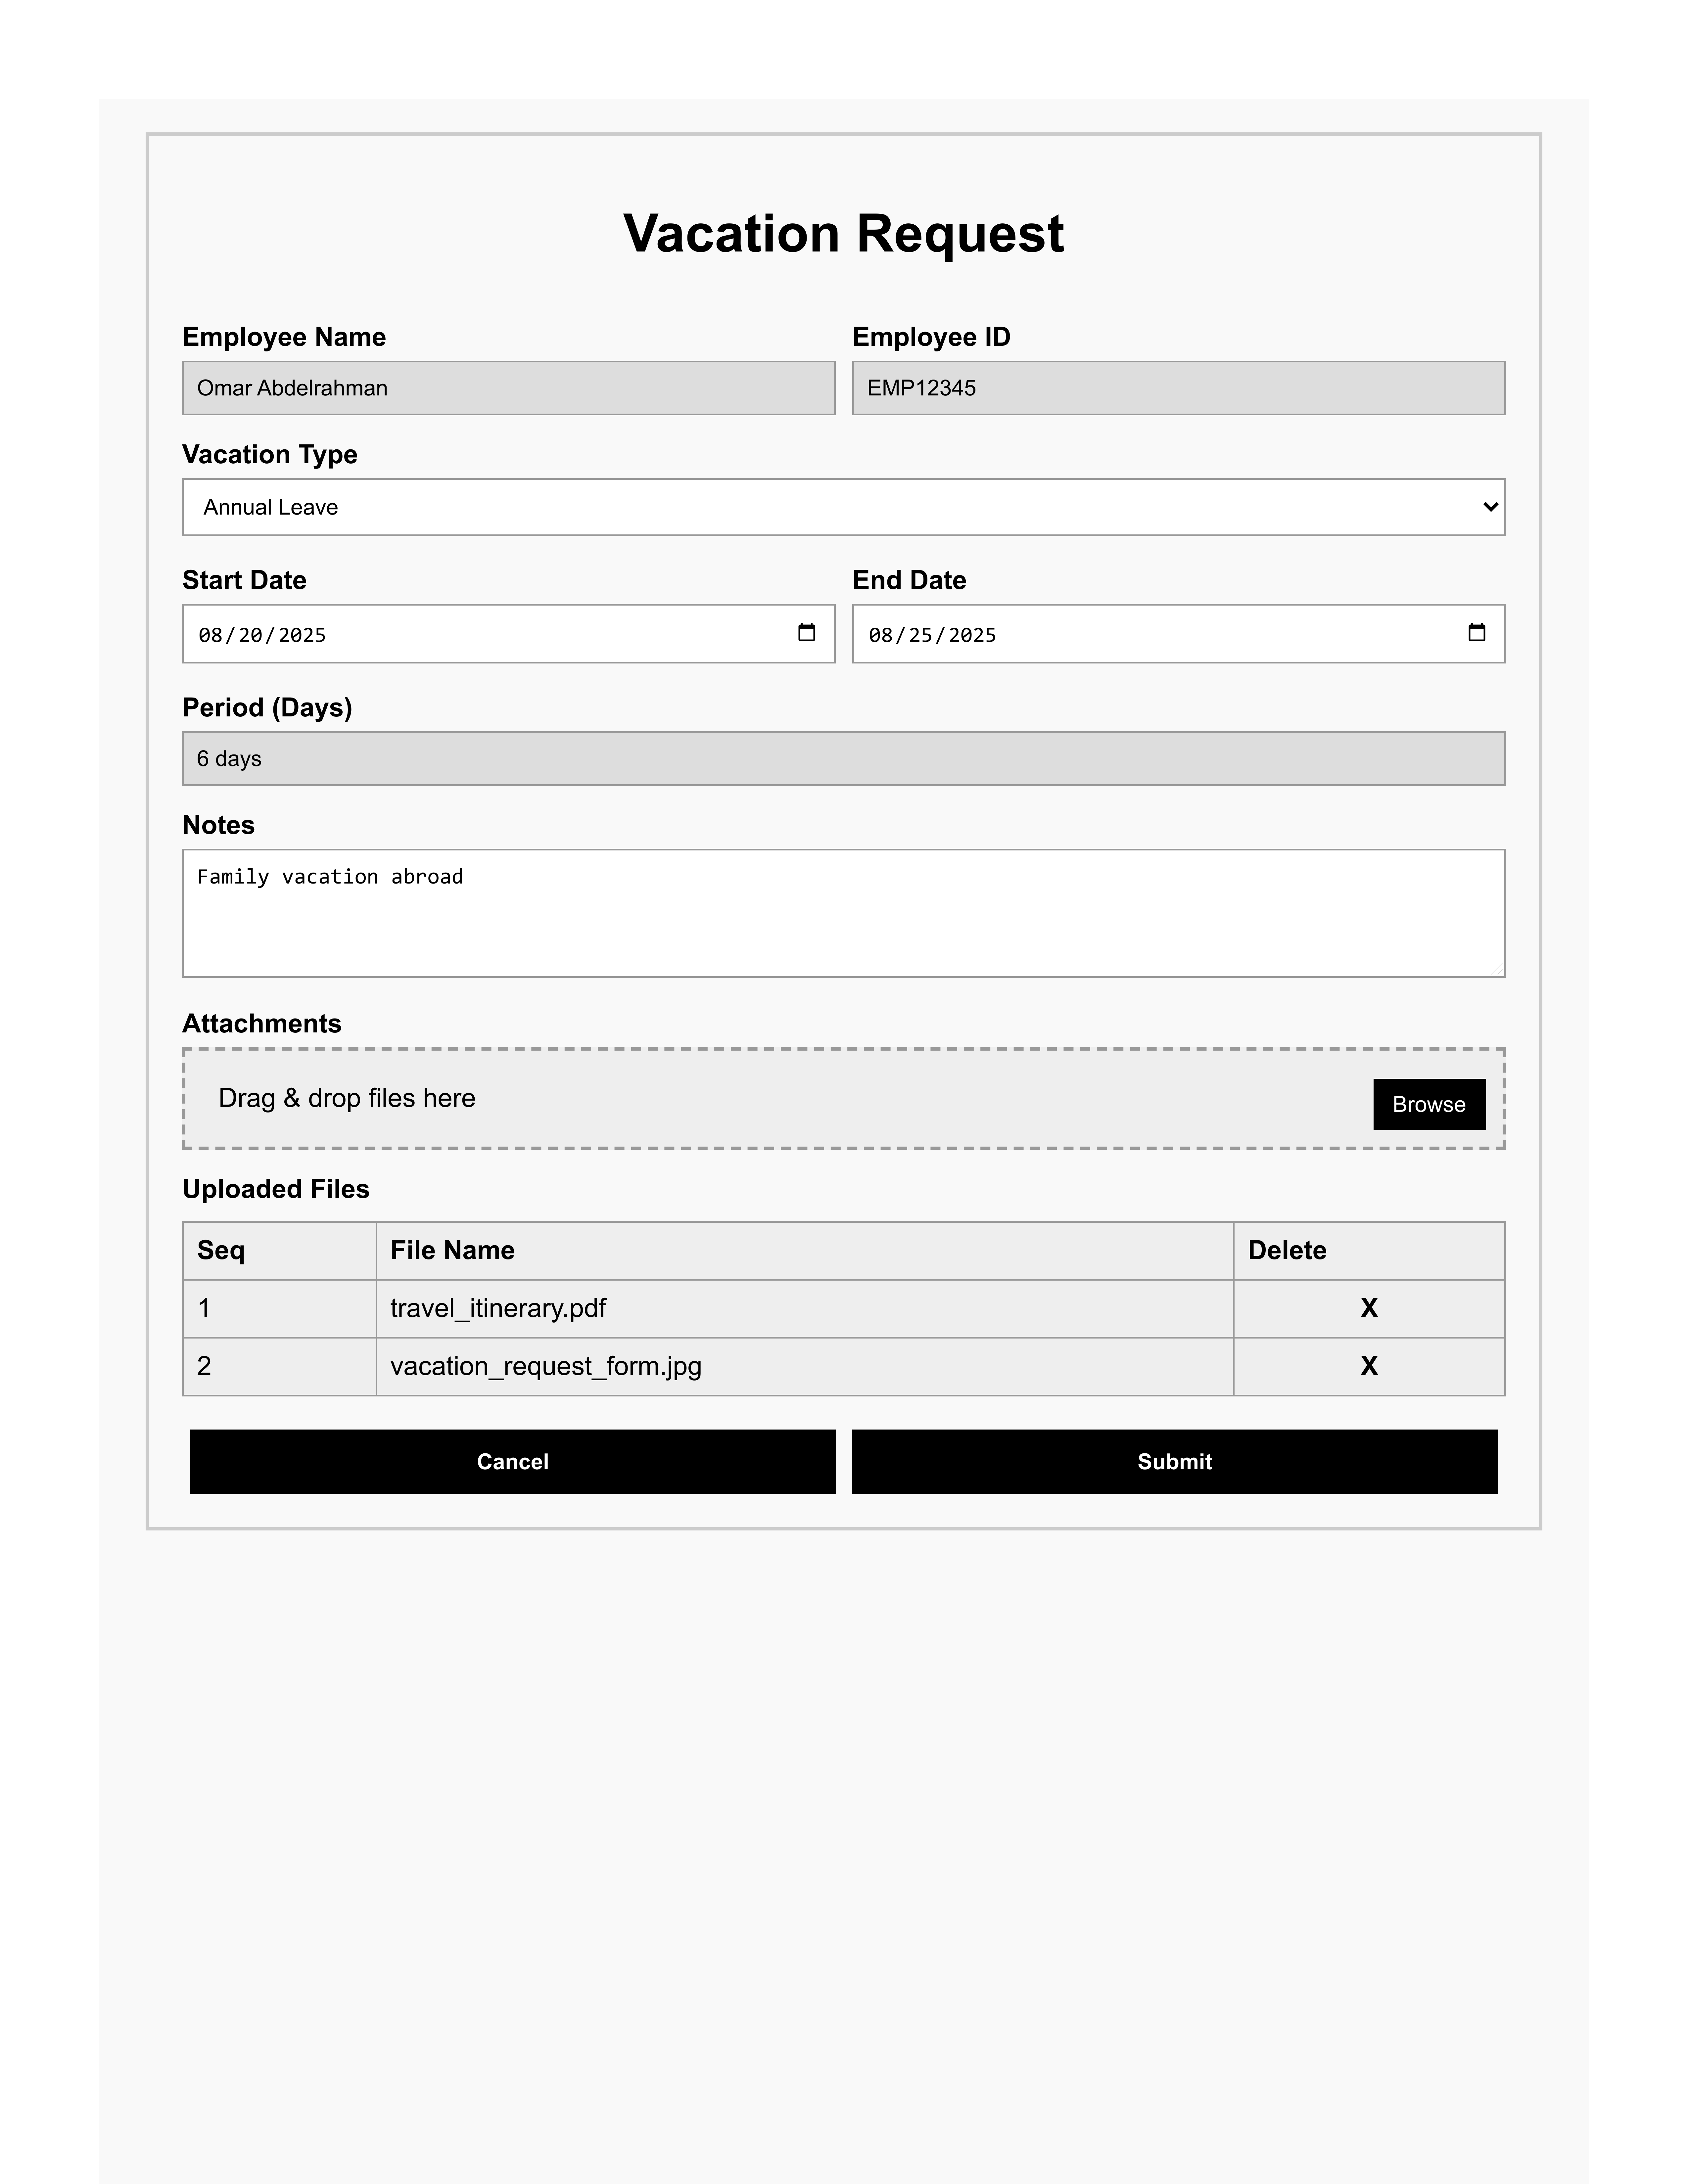
\includegraphics[width=0.8\textwidth]{Wireframes/Vacation-Request/Vacation-Request-1.png}
\caption{Vacation Request Screen}
\label{fig:vacation-request-screen}
\end{figure}

\subsubsection{Vacation Cancellation Request Screen}
\begin{figure}[H]
\centering
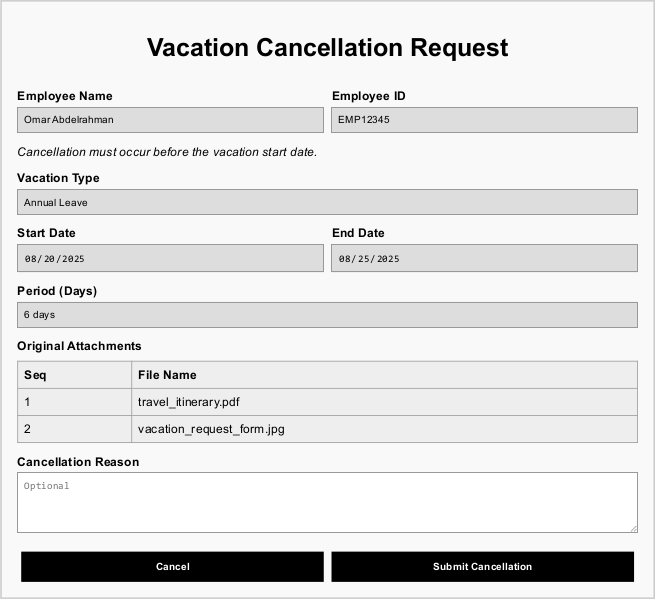
\includegraphics[width=0.8\textwidth]{Wireframes/Vacation-Cancellation-Request/Vacation-Cancellation-Request-1.png}
\caption{Vacation Cancellation Request Screen}
\label{fig:vacation-cancellation-screen}
\end{figure}

\subsubsection{Review Vacation Request Screen}
\begin{figure}[H]
\centering
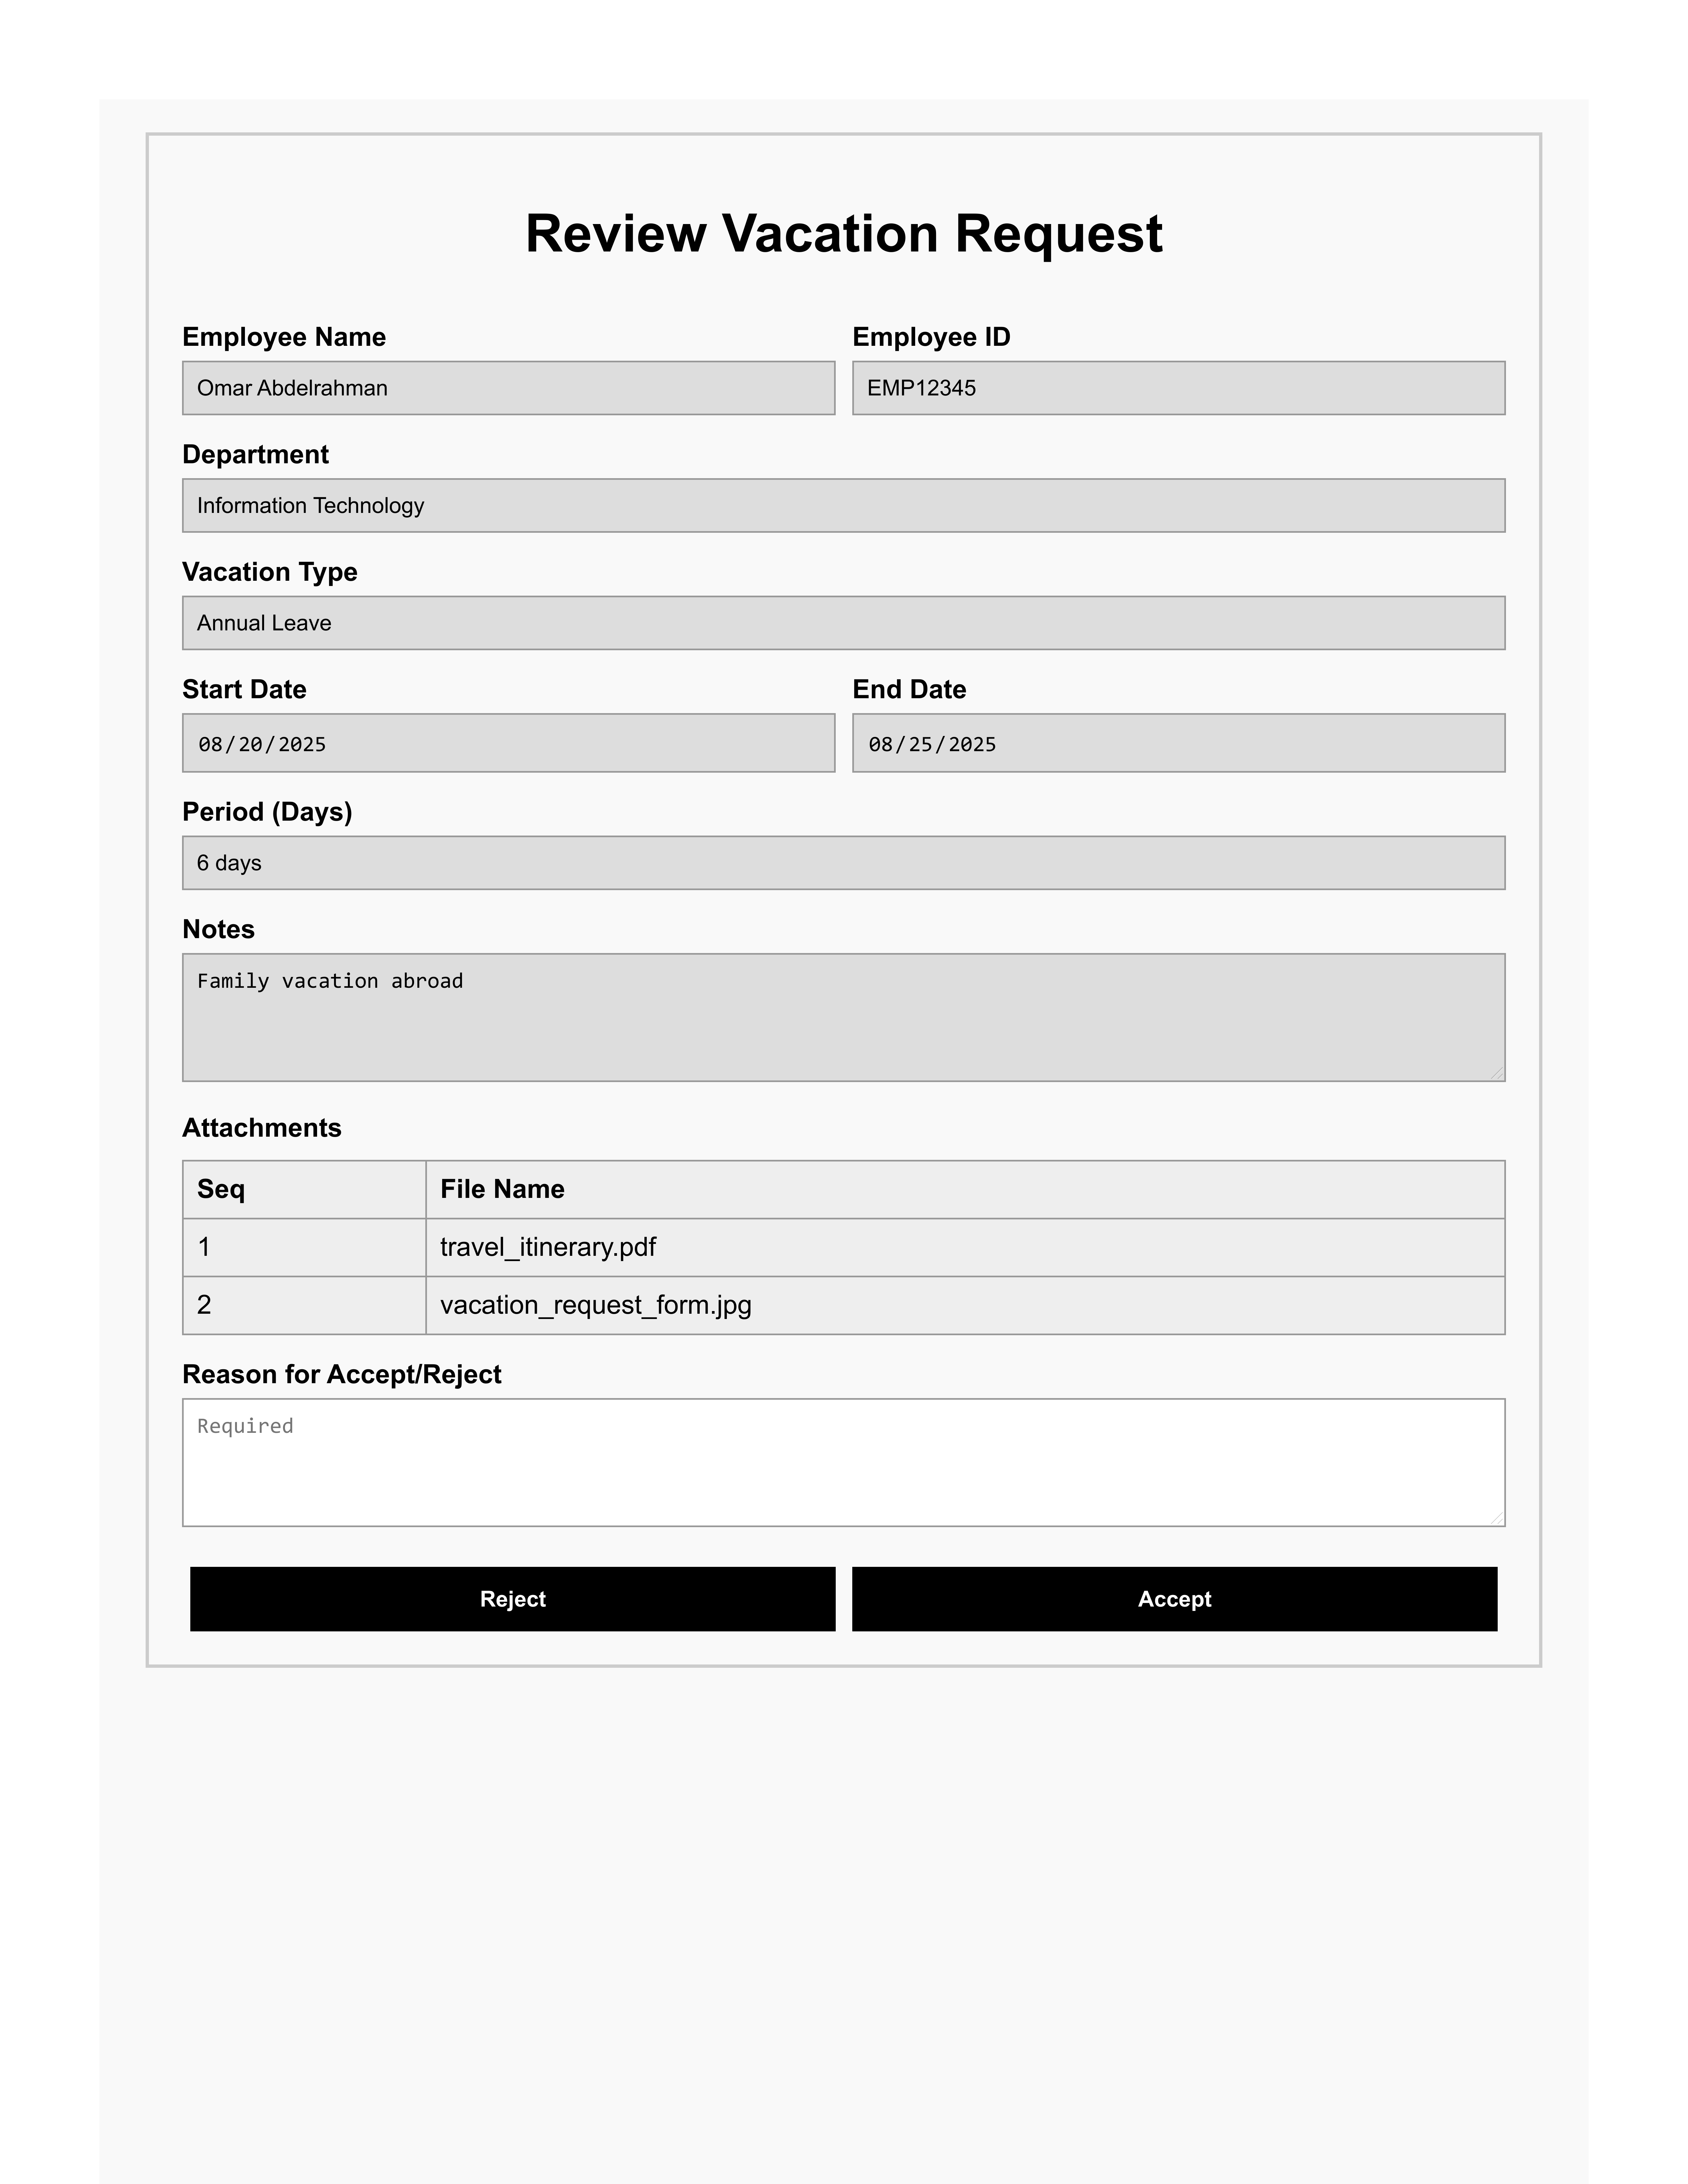
\includegraphics[width=0.8\textwidth]{Wireframes/Review-Vacation-Request/Review-Vacation-Request-1.png}
\caption{Review Vacation Request Screen}
\label{fig:review-vacation-screen}
\end{figure}

\subsubsection{Review Vacation Cancellation Request Screen}
\begin{figure}[H]
\centering
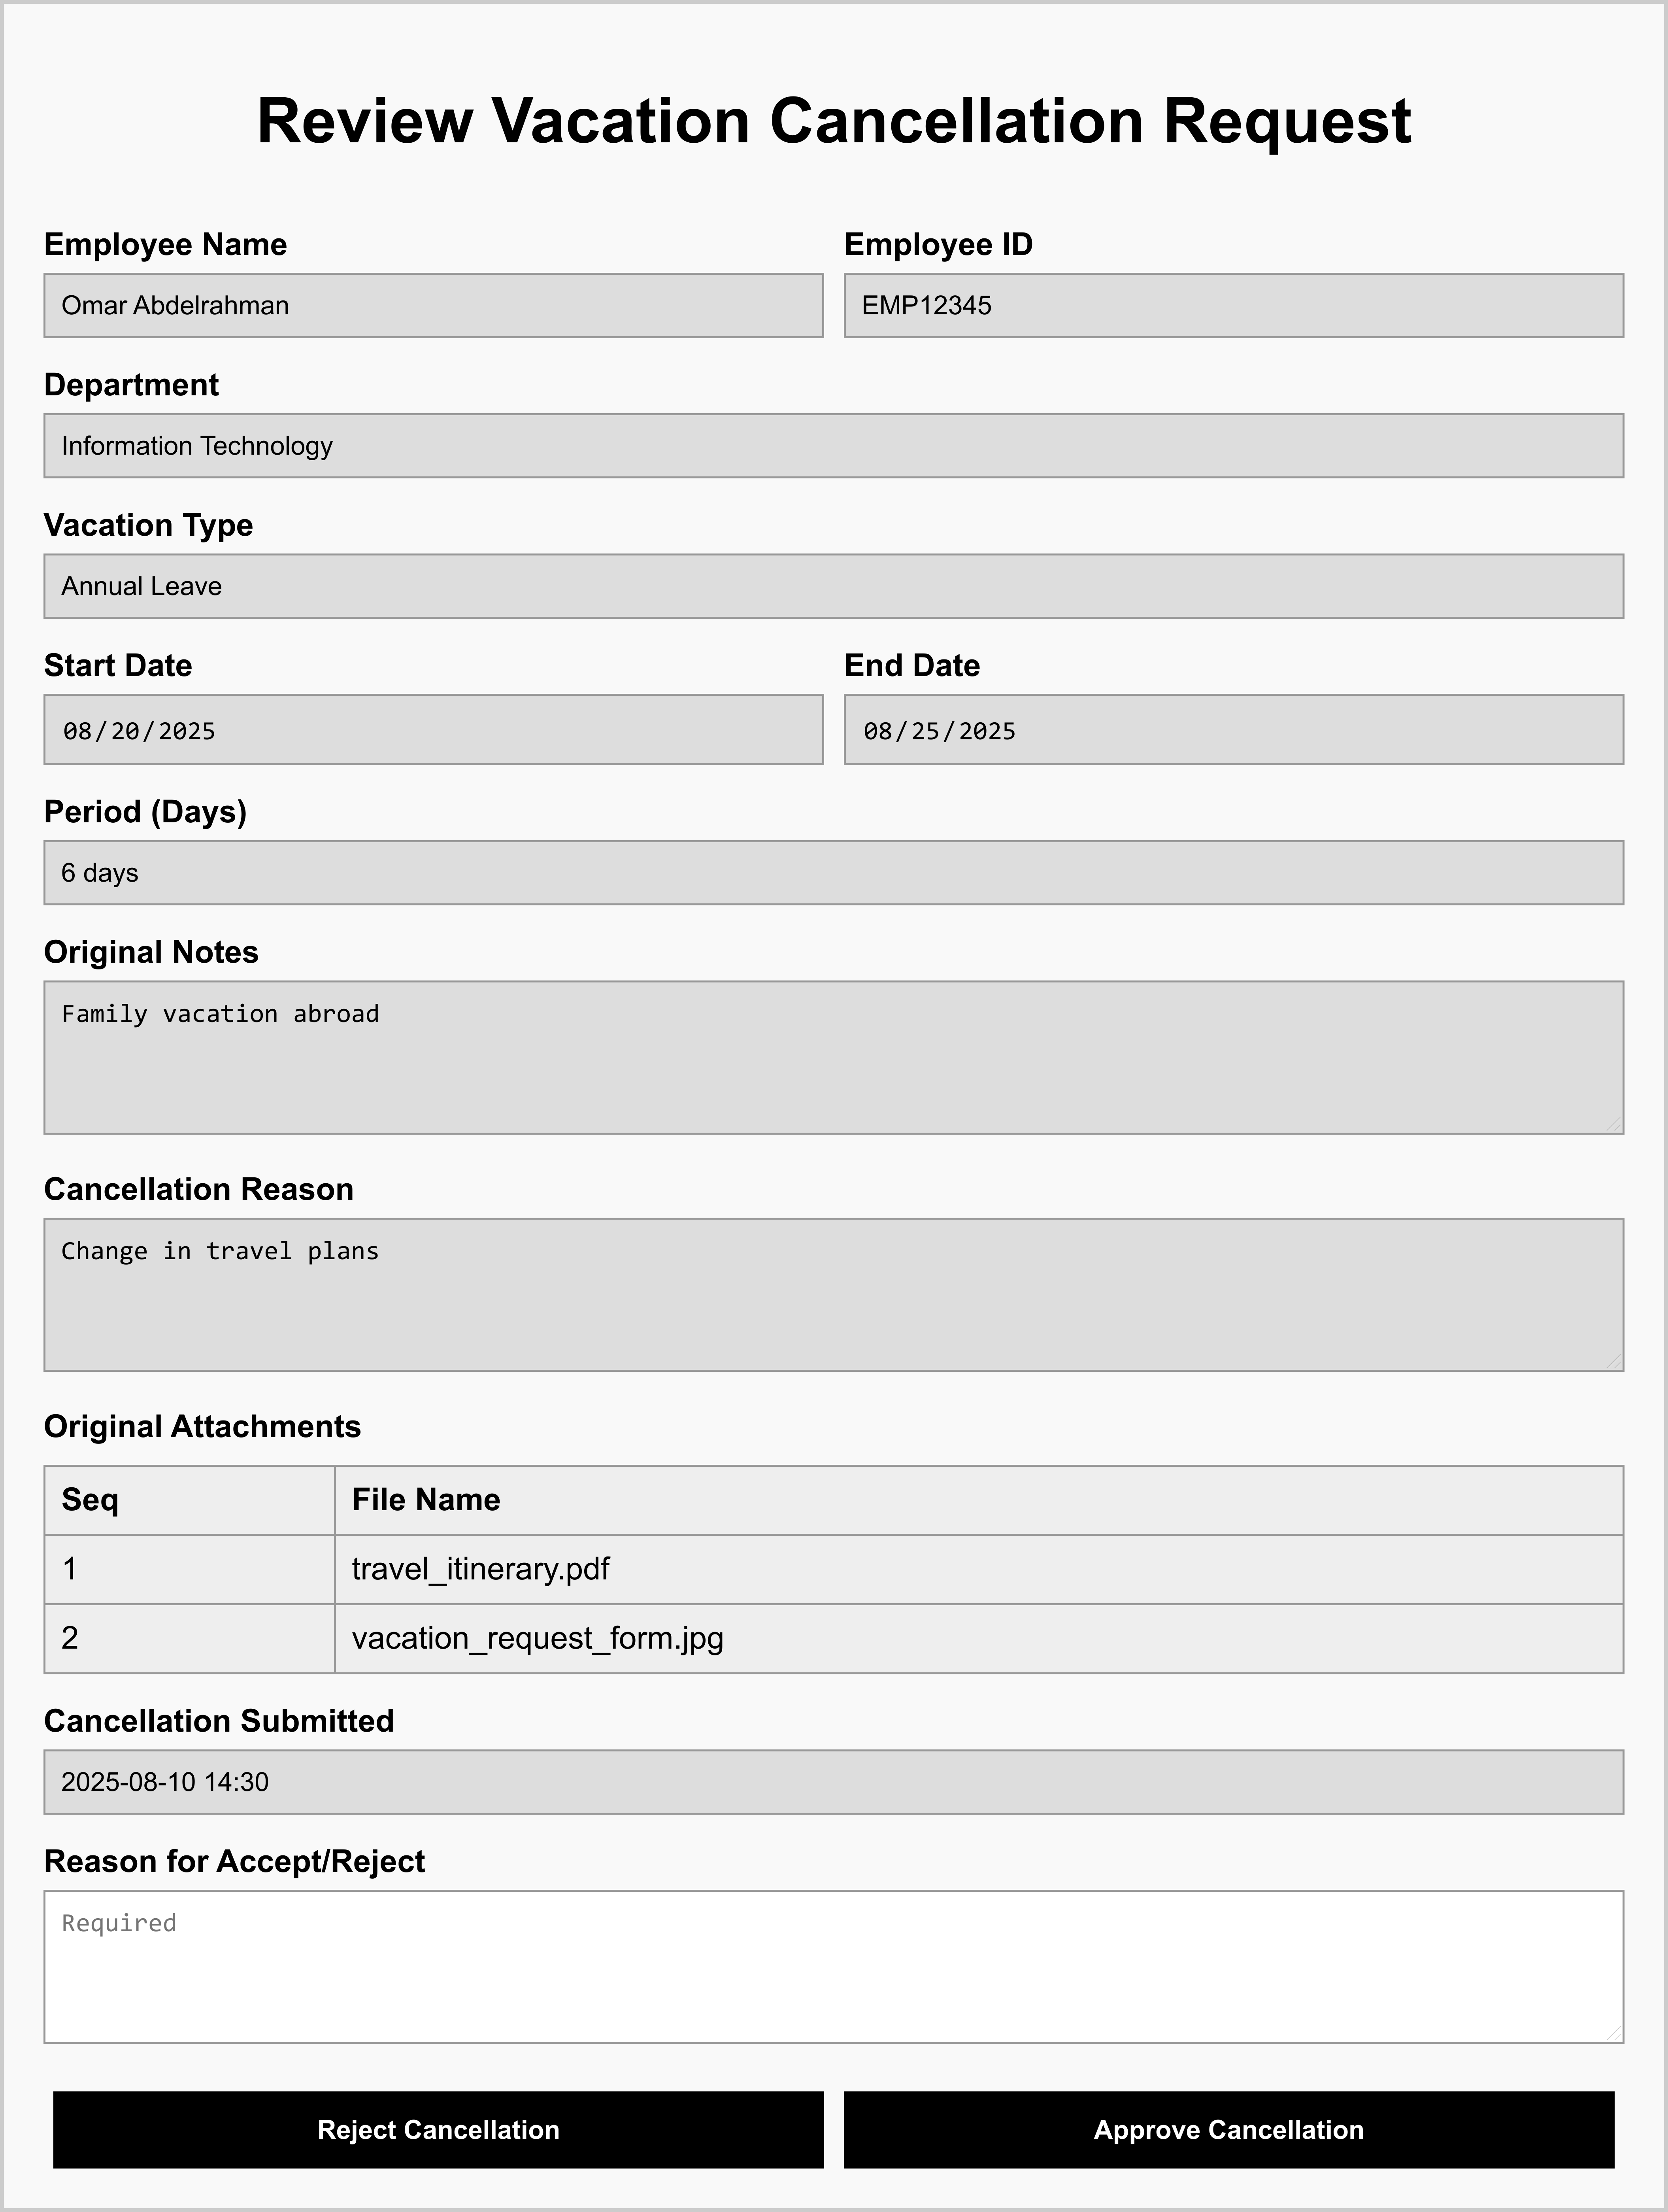
\includegraphics[width=0.8\textwidth]{Wireframes/Review-Vacation-Cancellation-Request/Review-Vacation-Cancellation-Request-1.png}
\caption{Review Vacation Cancellation Request Screen}
\label{fig:review-cancellation-screen}
\end{figure}

\subsubsection{My Vacation Requests Screen}
\begin{figure}[H]
\centering
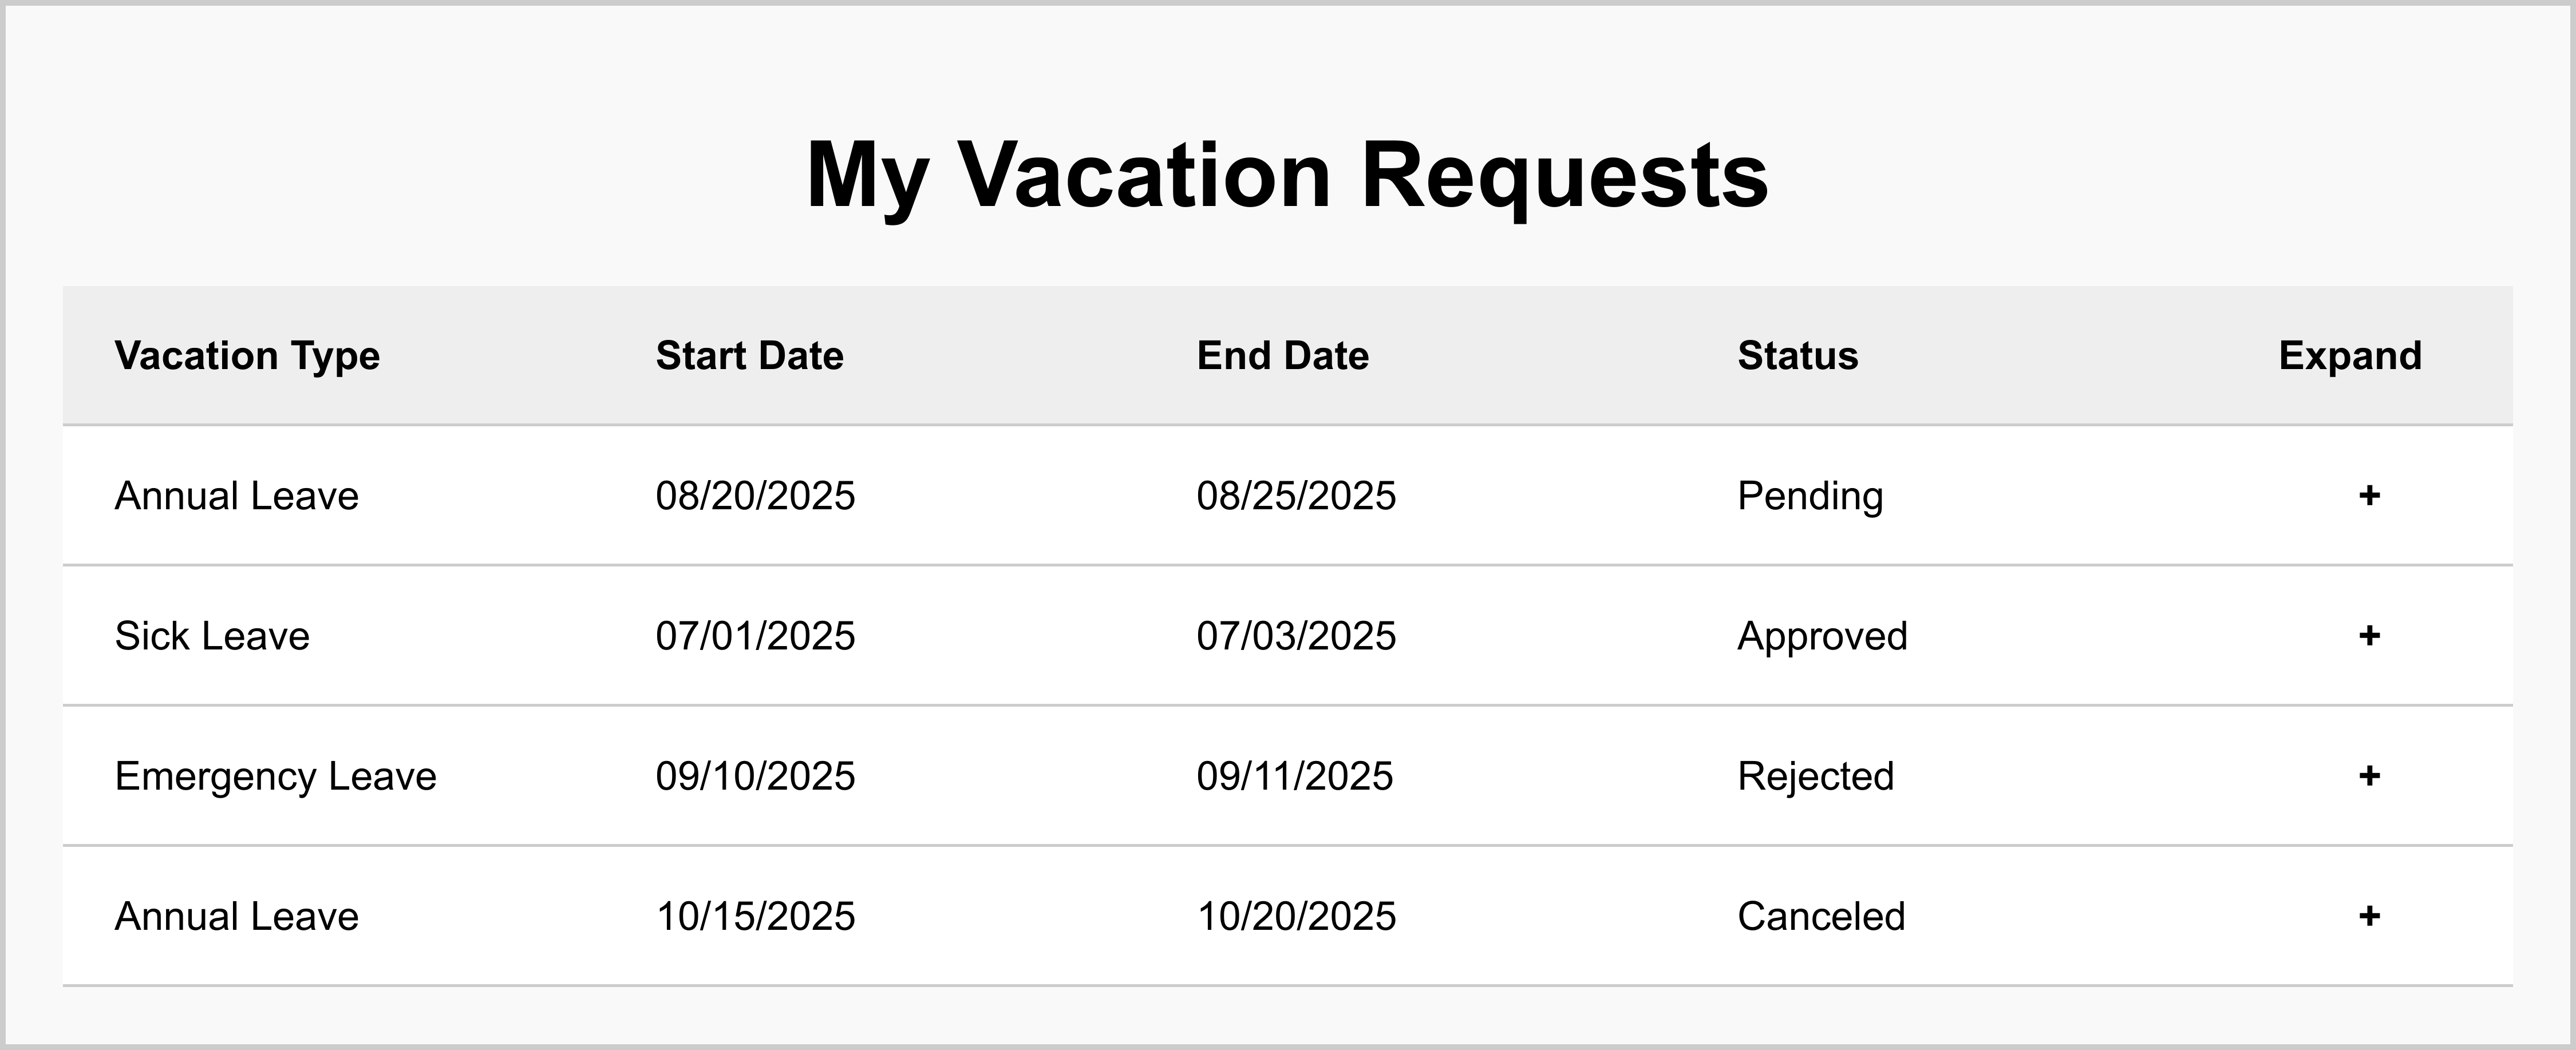
\includegraphics[width=0.8\textwidth]{Wireframes/My-Vacation-Requests/My-Vacation-Requests-1.png}
\caption{My Vacation Requests Screen}
\label{fig:my-vacation-requests-screen}
\end{figure}

\subsubsection{Pending Vacation Requests Screen}
\begin{figure}[H]
\centering
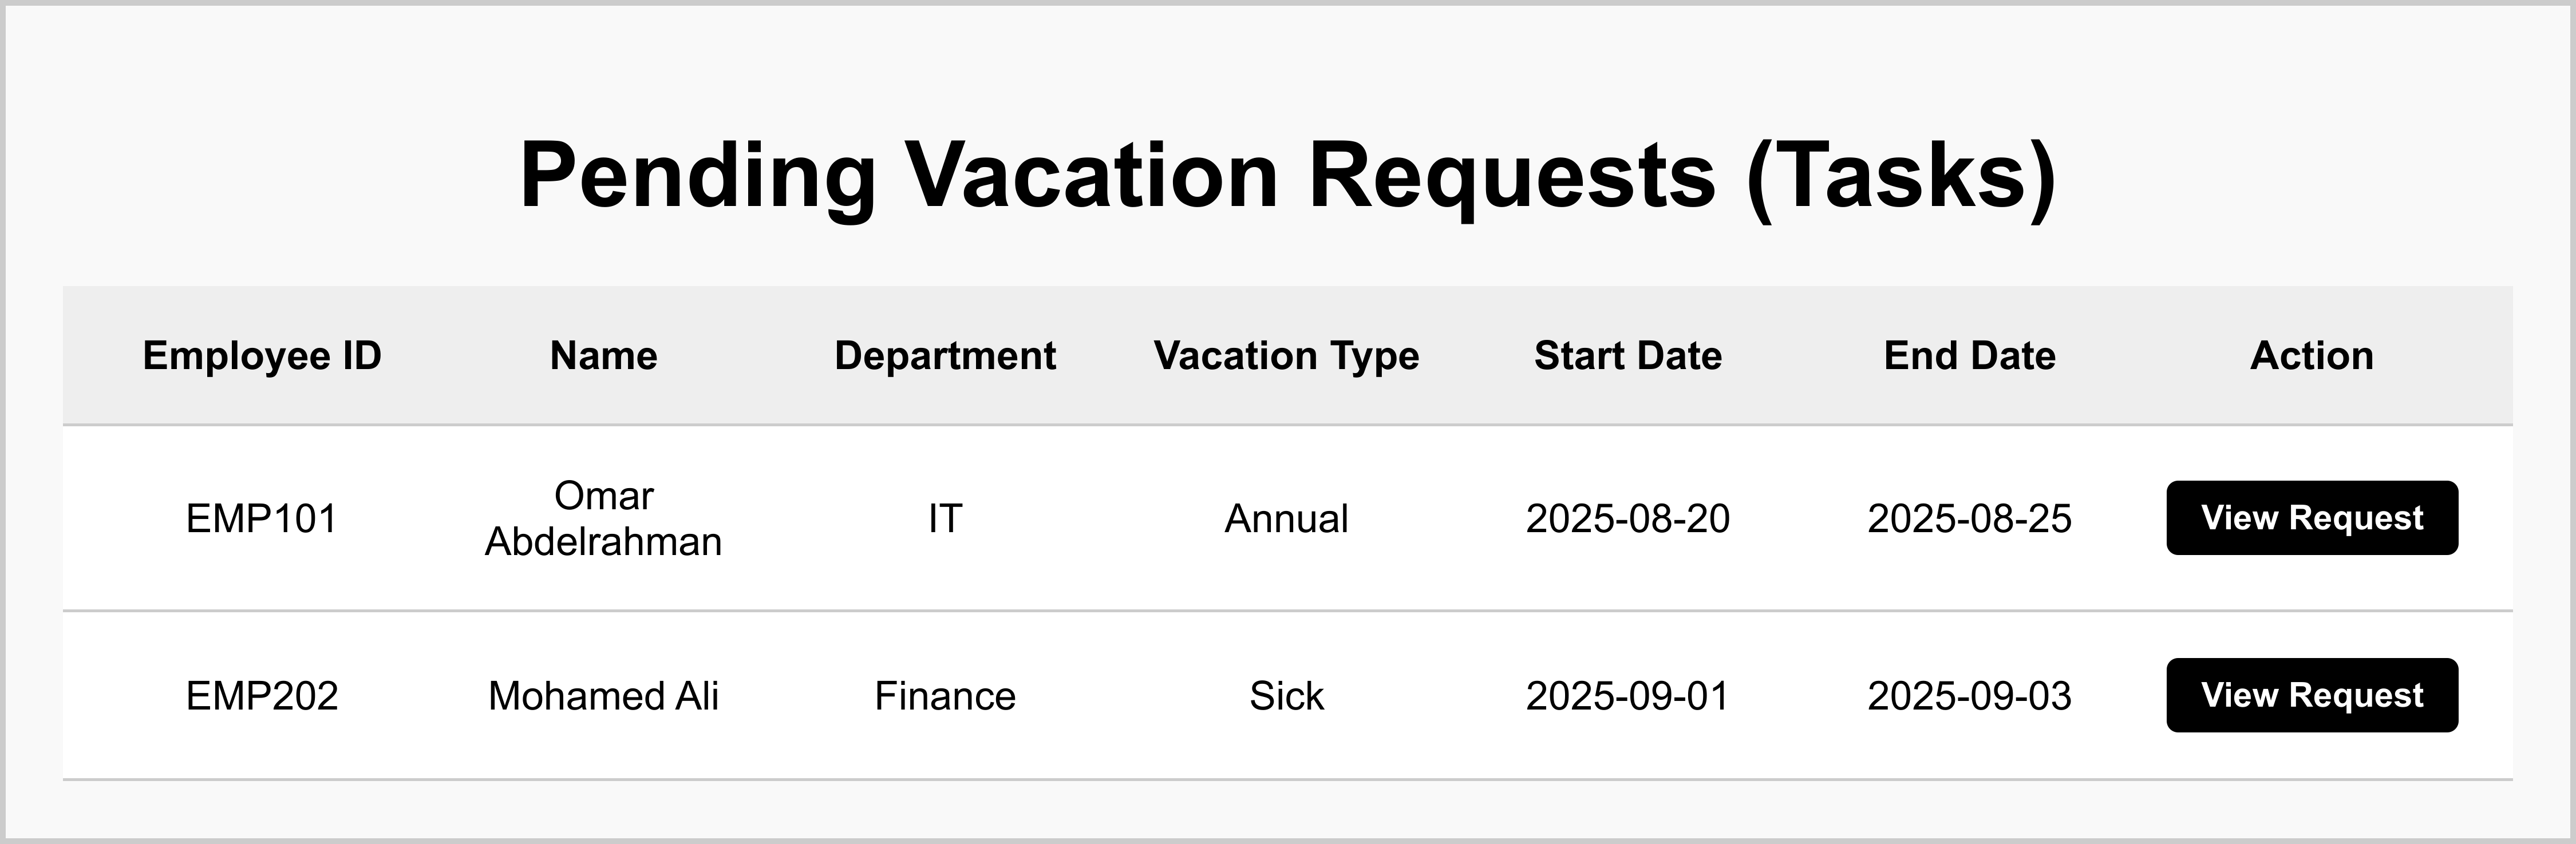
\includegraphics[width=0.8\textwidth]{Wireframes/Pending-Vacation-Requests/Pending-Vacation-Requests-1.png}
\caption{Pending Vacation Requests Screen}
\label{fig:pending-vacation-requests-screen}
\end{figure}

\subsubsection{Vacation Inquiry Search Parameters Screen}
\begin{figure}[H]
\centering
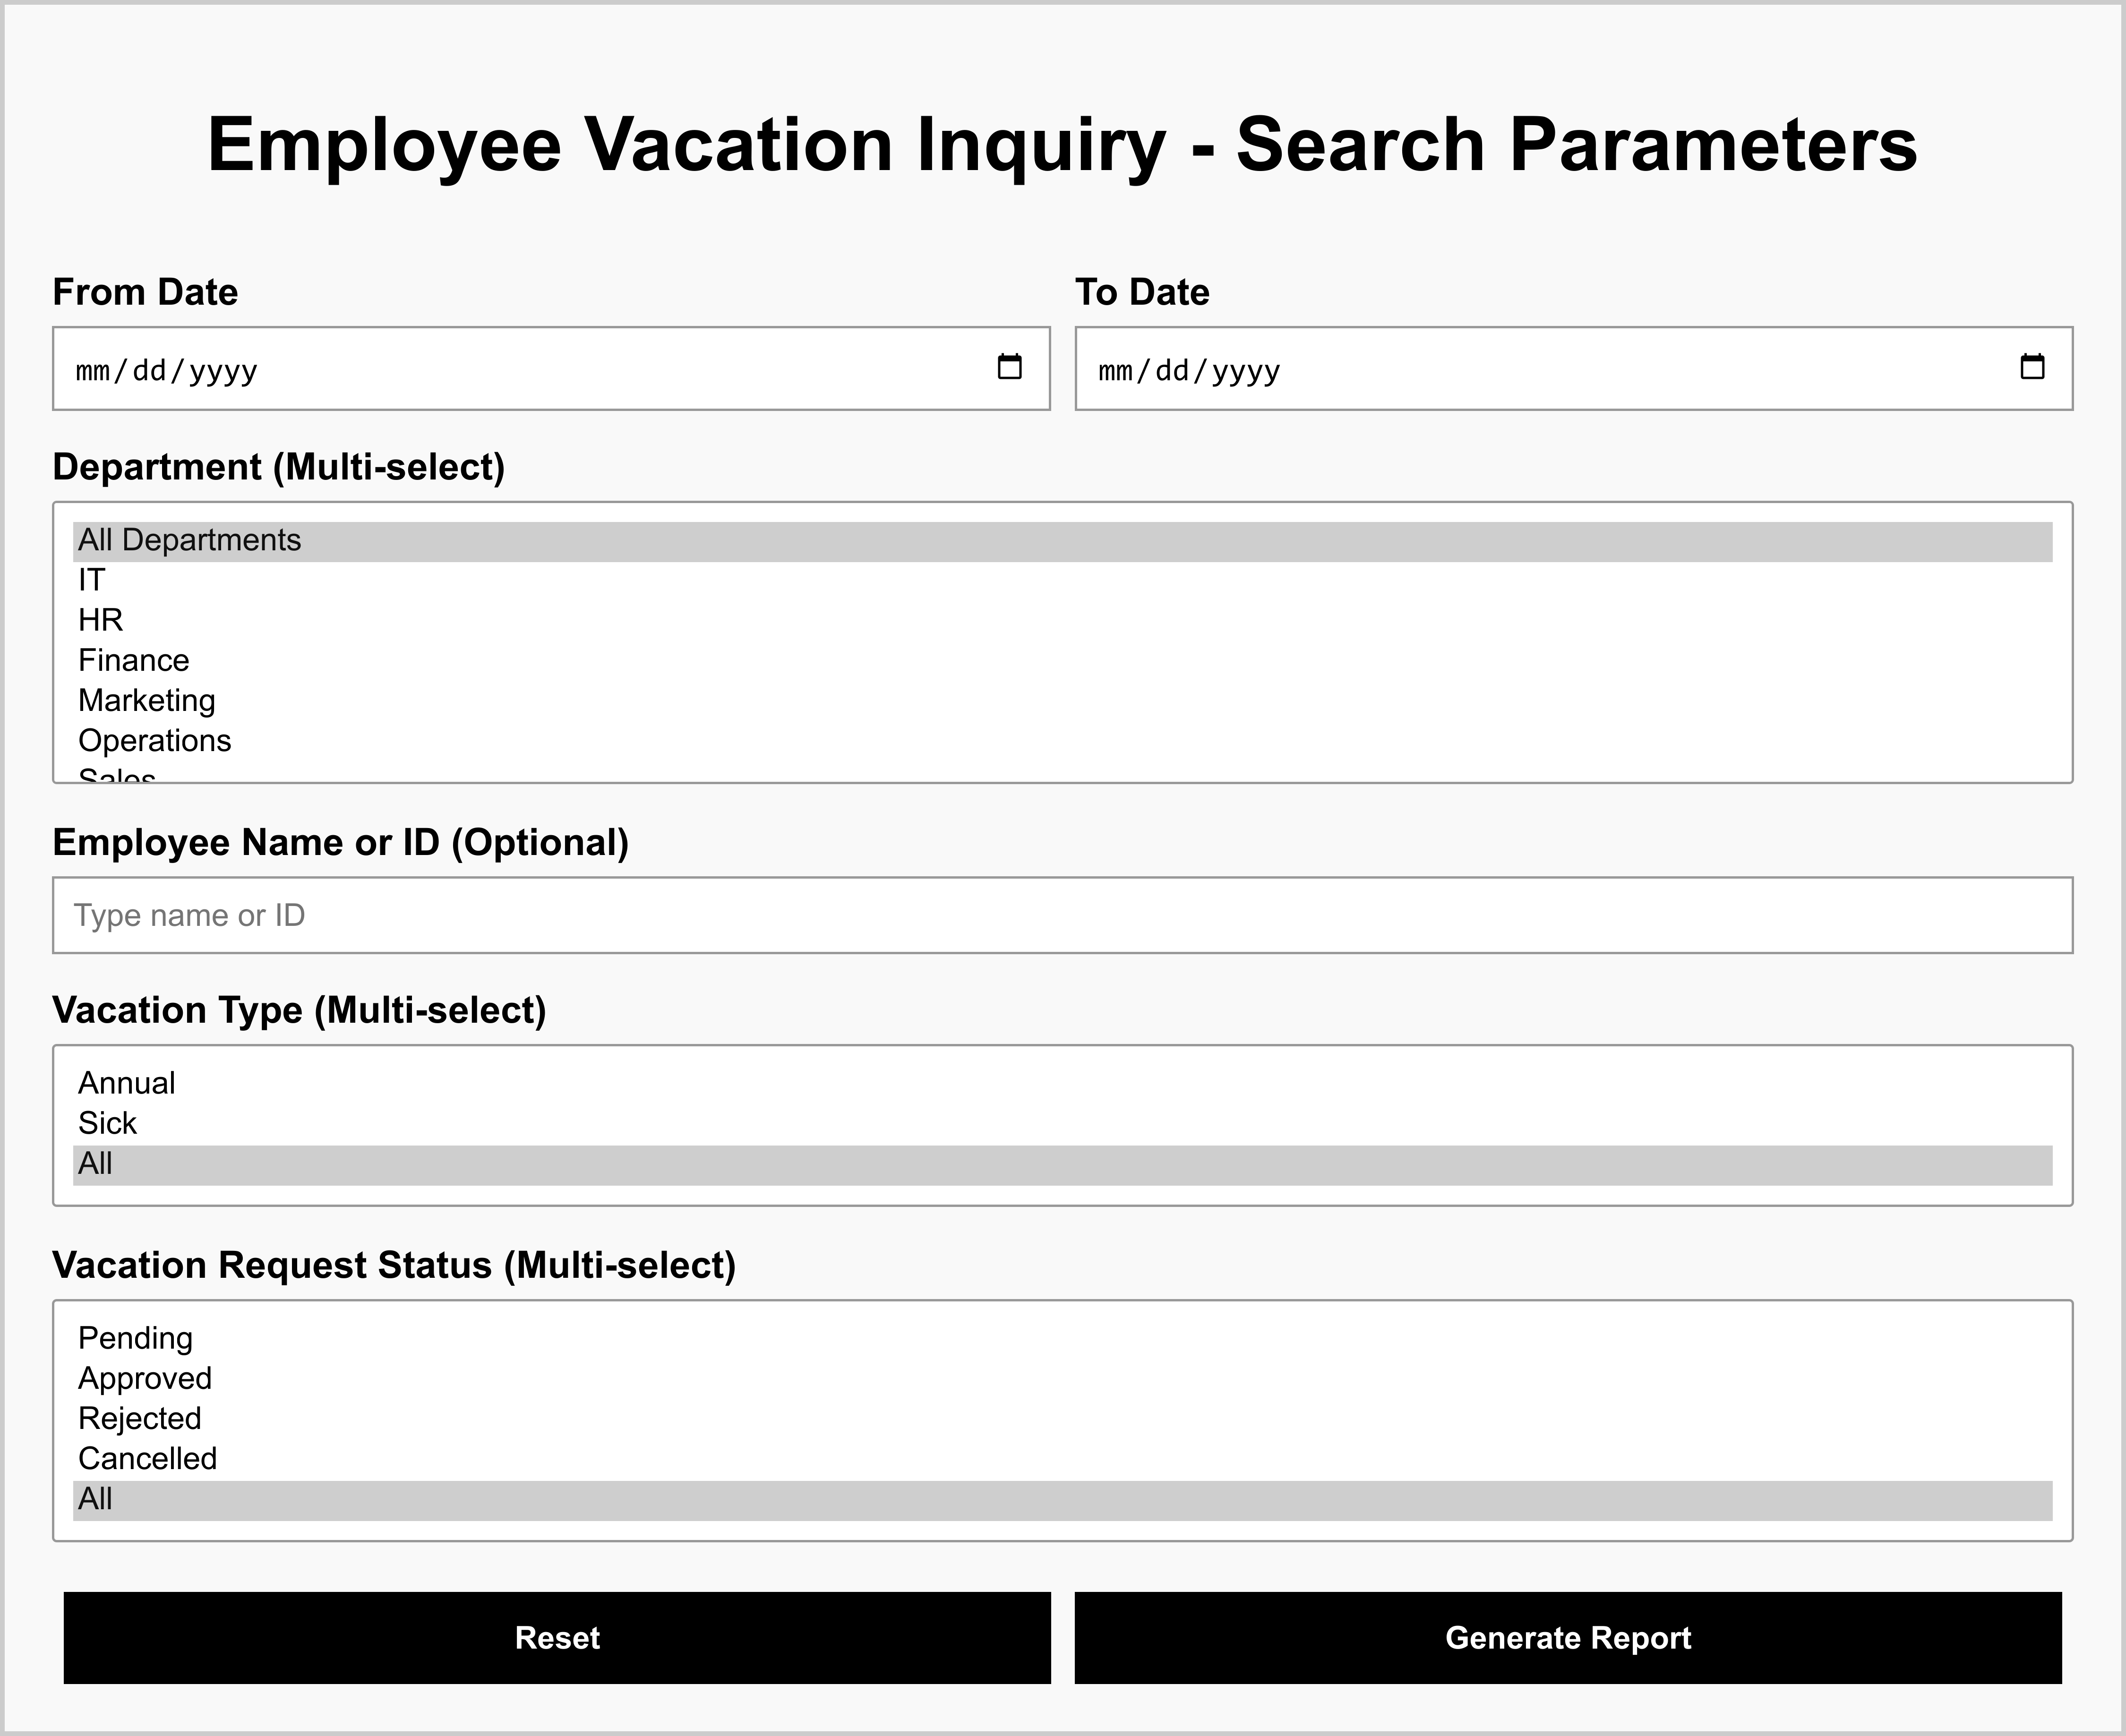
\includegraphics[width=0.8\textwidth]{Wireframes/Employee-Vacation-Inquiry-Search-Parameters/Employee-Vacation-Inquiry-Search-Parameters-1.png}
\caption{Vacation Inquiry Search Parameters Screen}
\label{fig:inquiry-search-params-screen}
\end{figure}

\subsubsection{Vacation Inquiry Search Results Screen}
\begin{figure}[H]
\centering
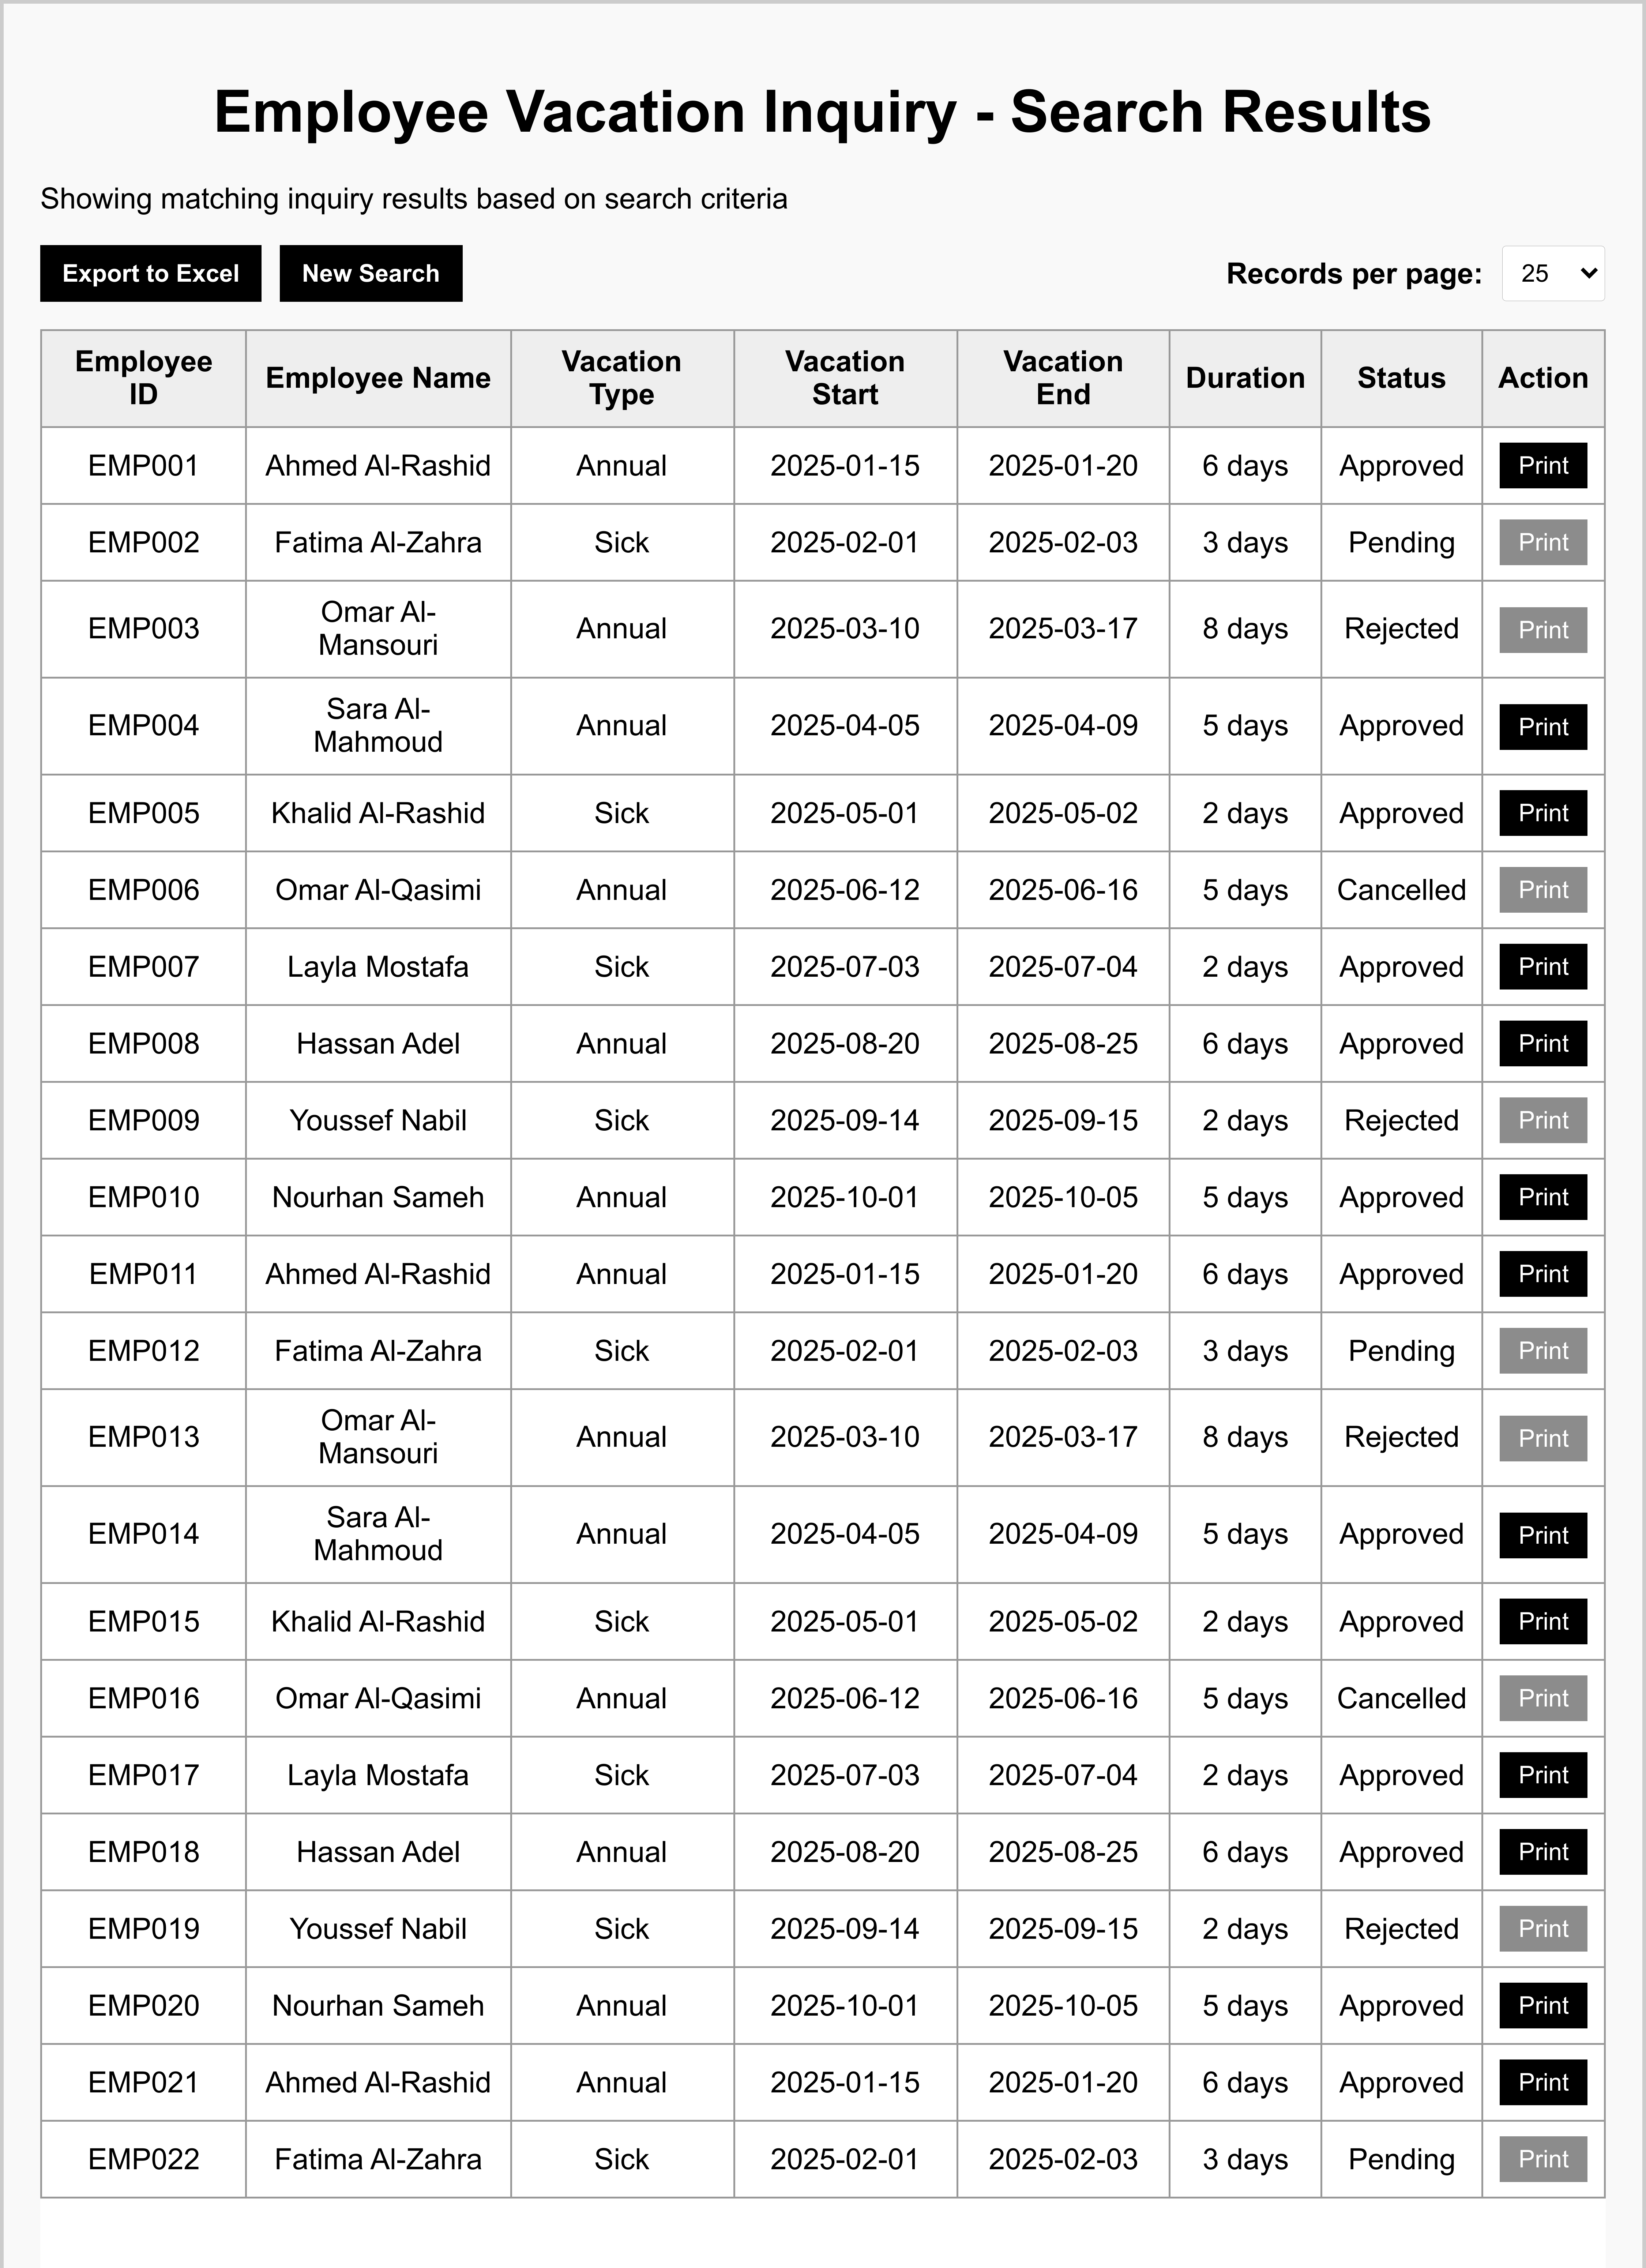
\includegraphics[width=0.8\textwidth]{Wireframes/Employee-Vacation-Inquiry-Search-Results/Employee-Vacation-Inquiry-Search-Results-1.png}
\caption{Vacation Inquiry Search Results Screen}
\label{fig:inquiry-search-results-screen}
\end{figure}

\subsubsection{Notifications Center Screen}
\begin{figure}[H]
\centering
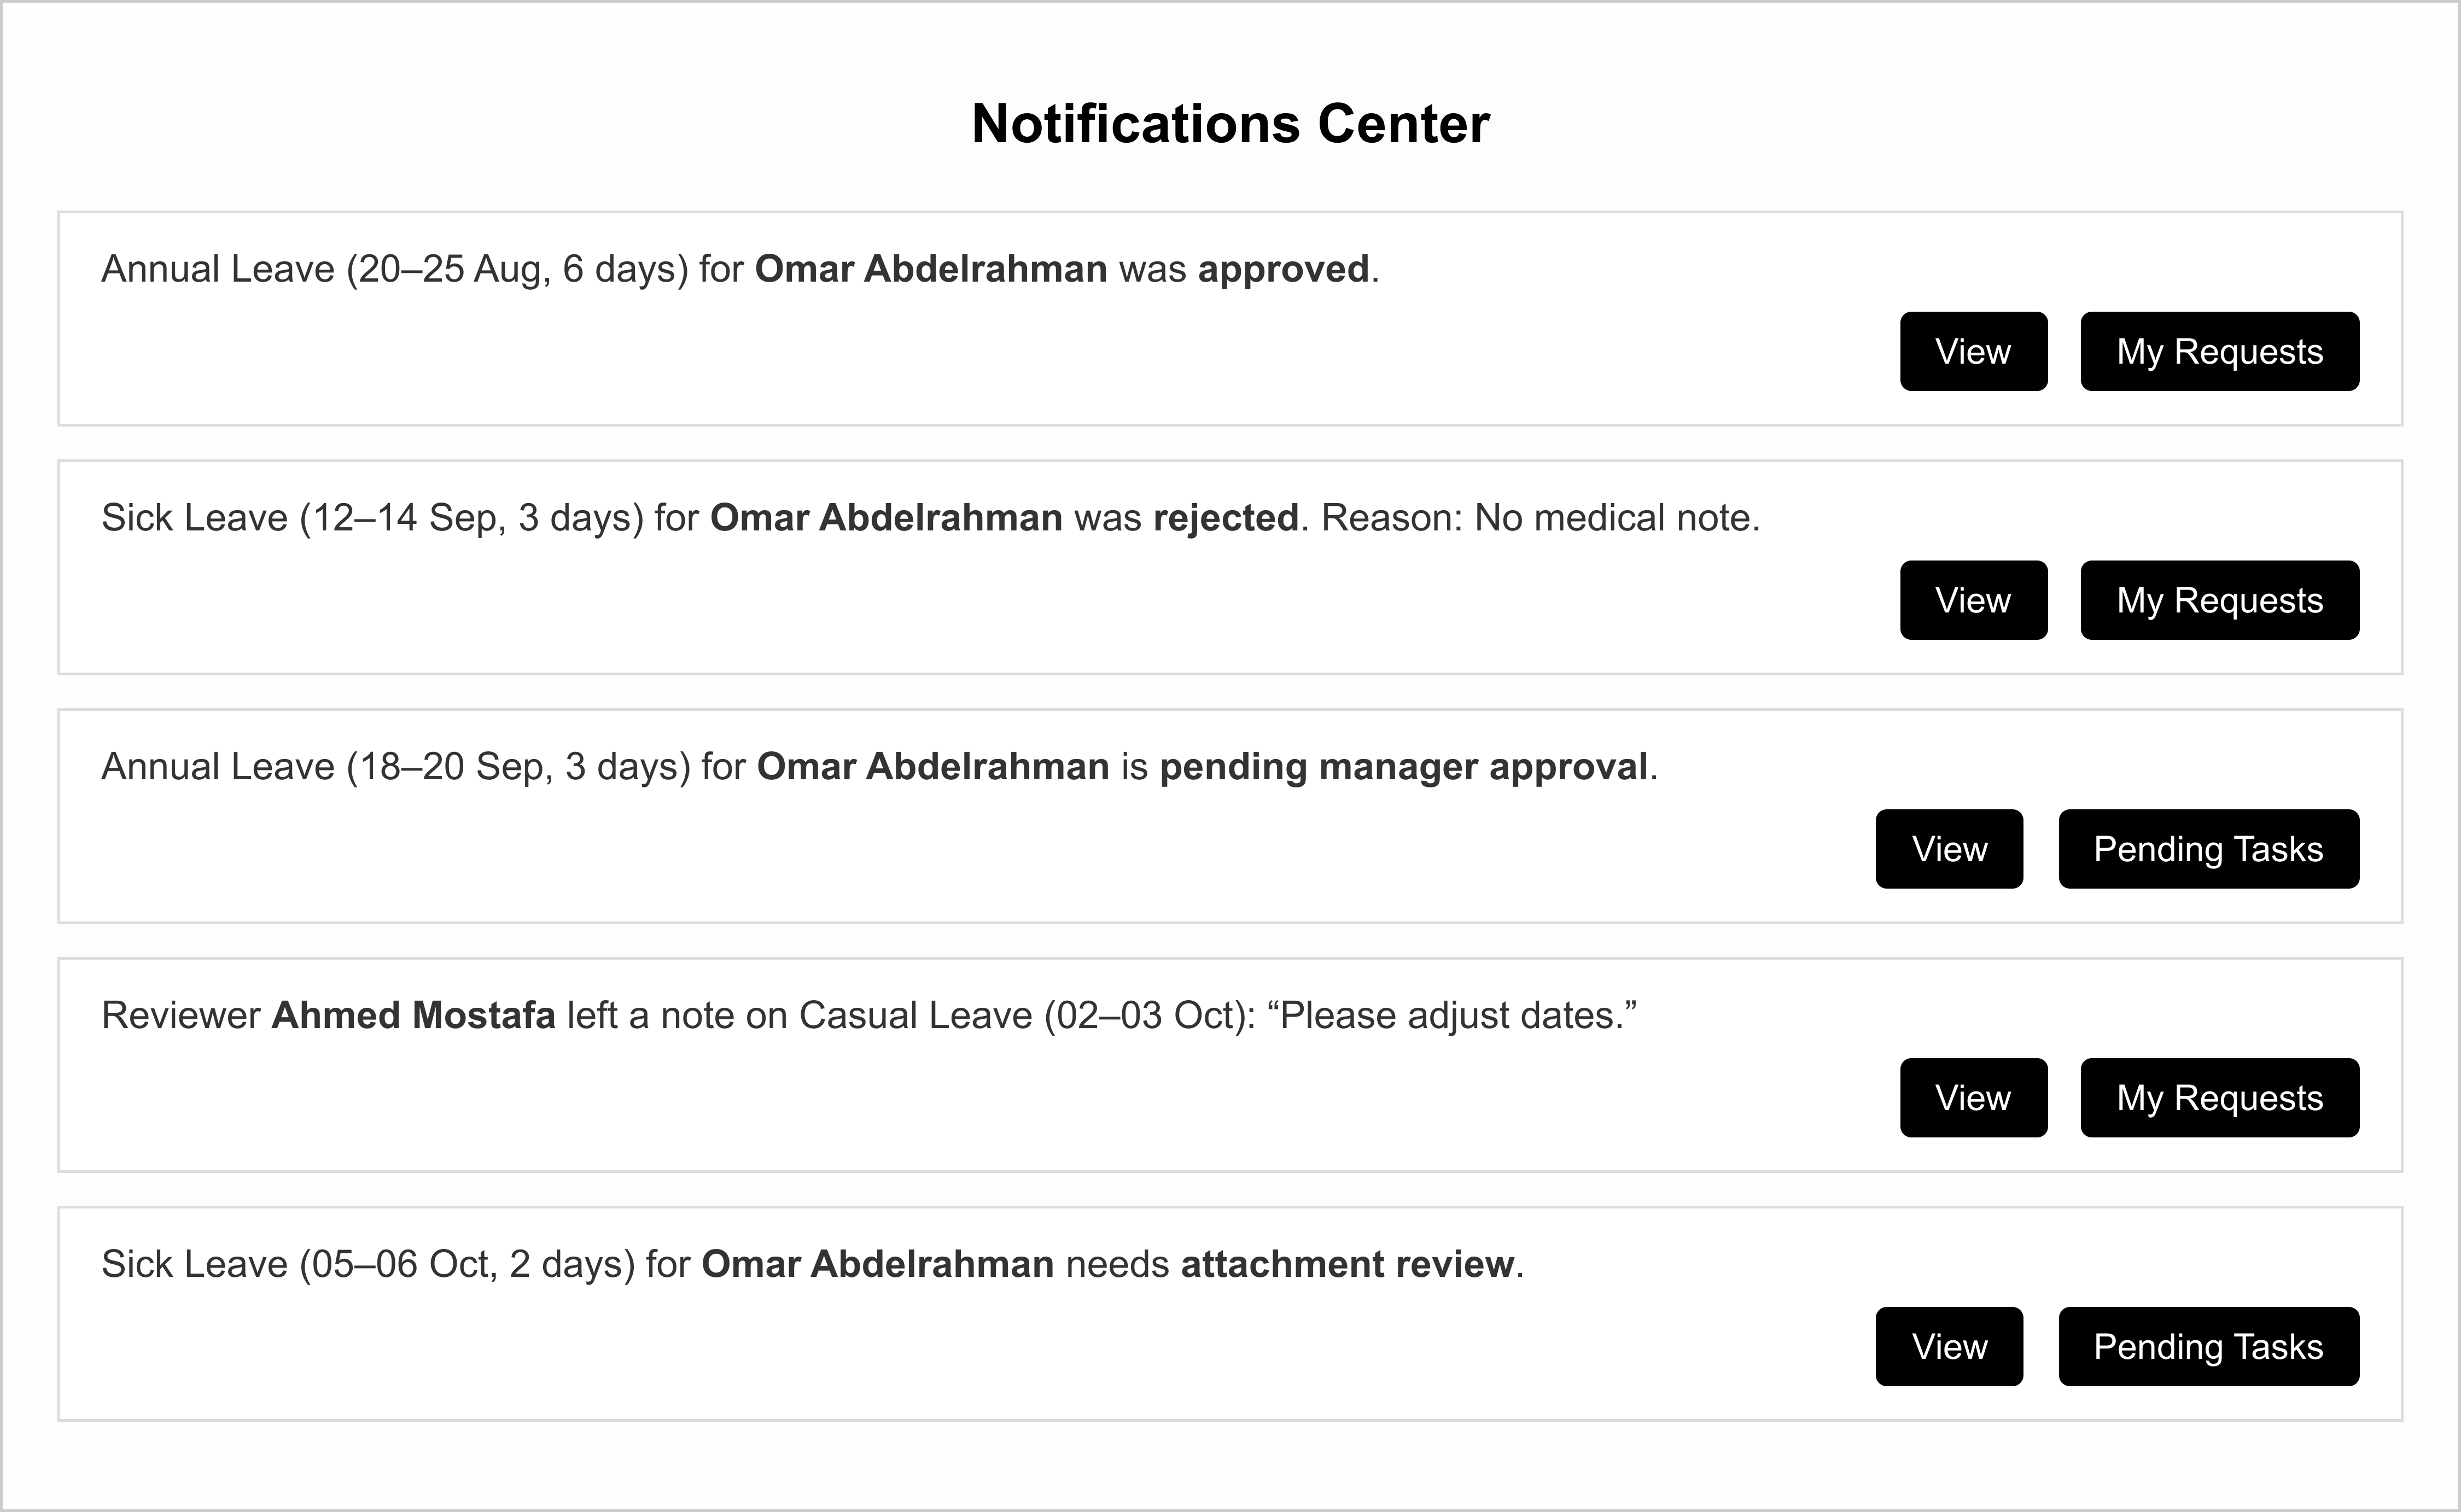
\includegraphics[width=0.8\textwidth]{Wireframes/Notifications-Center/Notifications-Center-1.png}
\caption{Notifications Center Screen}
\label{fig:notifications-center-screen}
\end{figure}

\subsection{Report Layout Screens}

\subsubsection{Single Transaction Report Layout}
\begin{figure}[H]
\centering
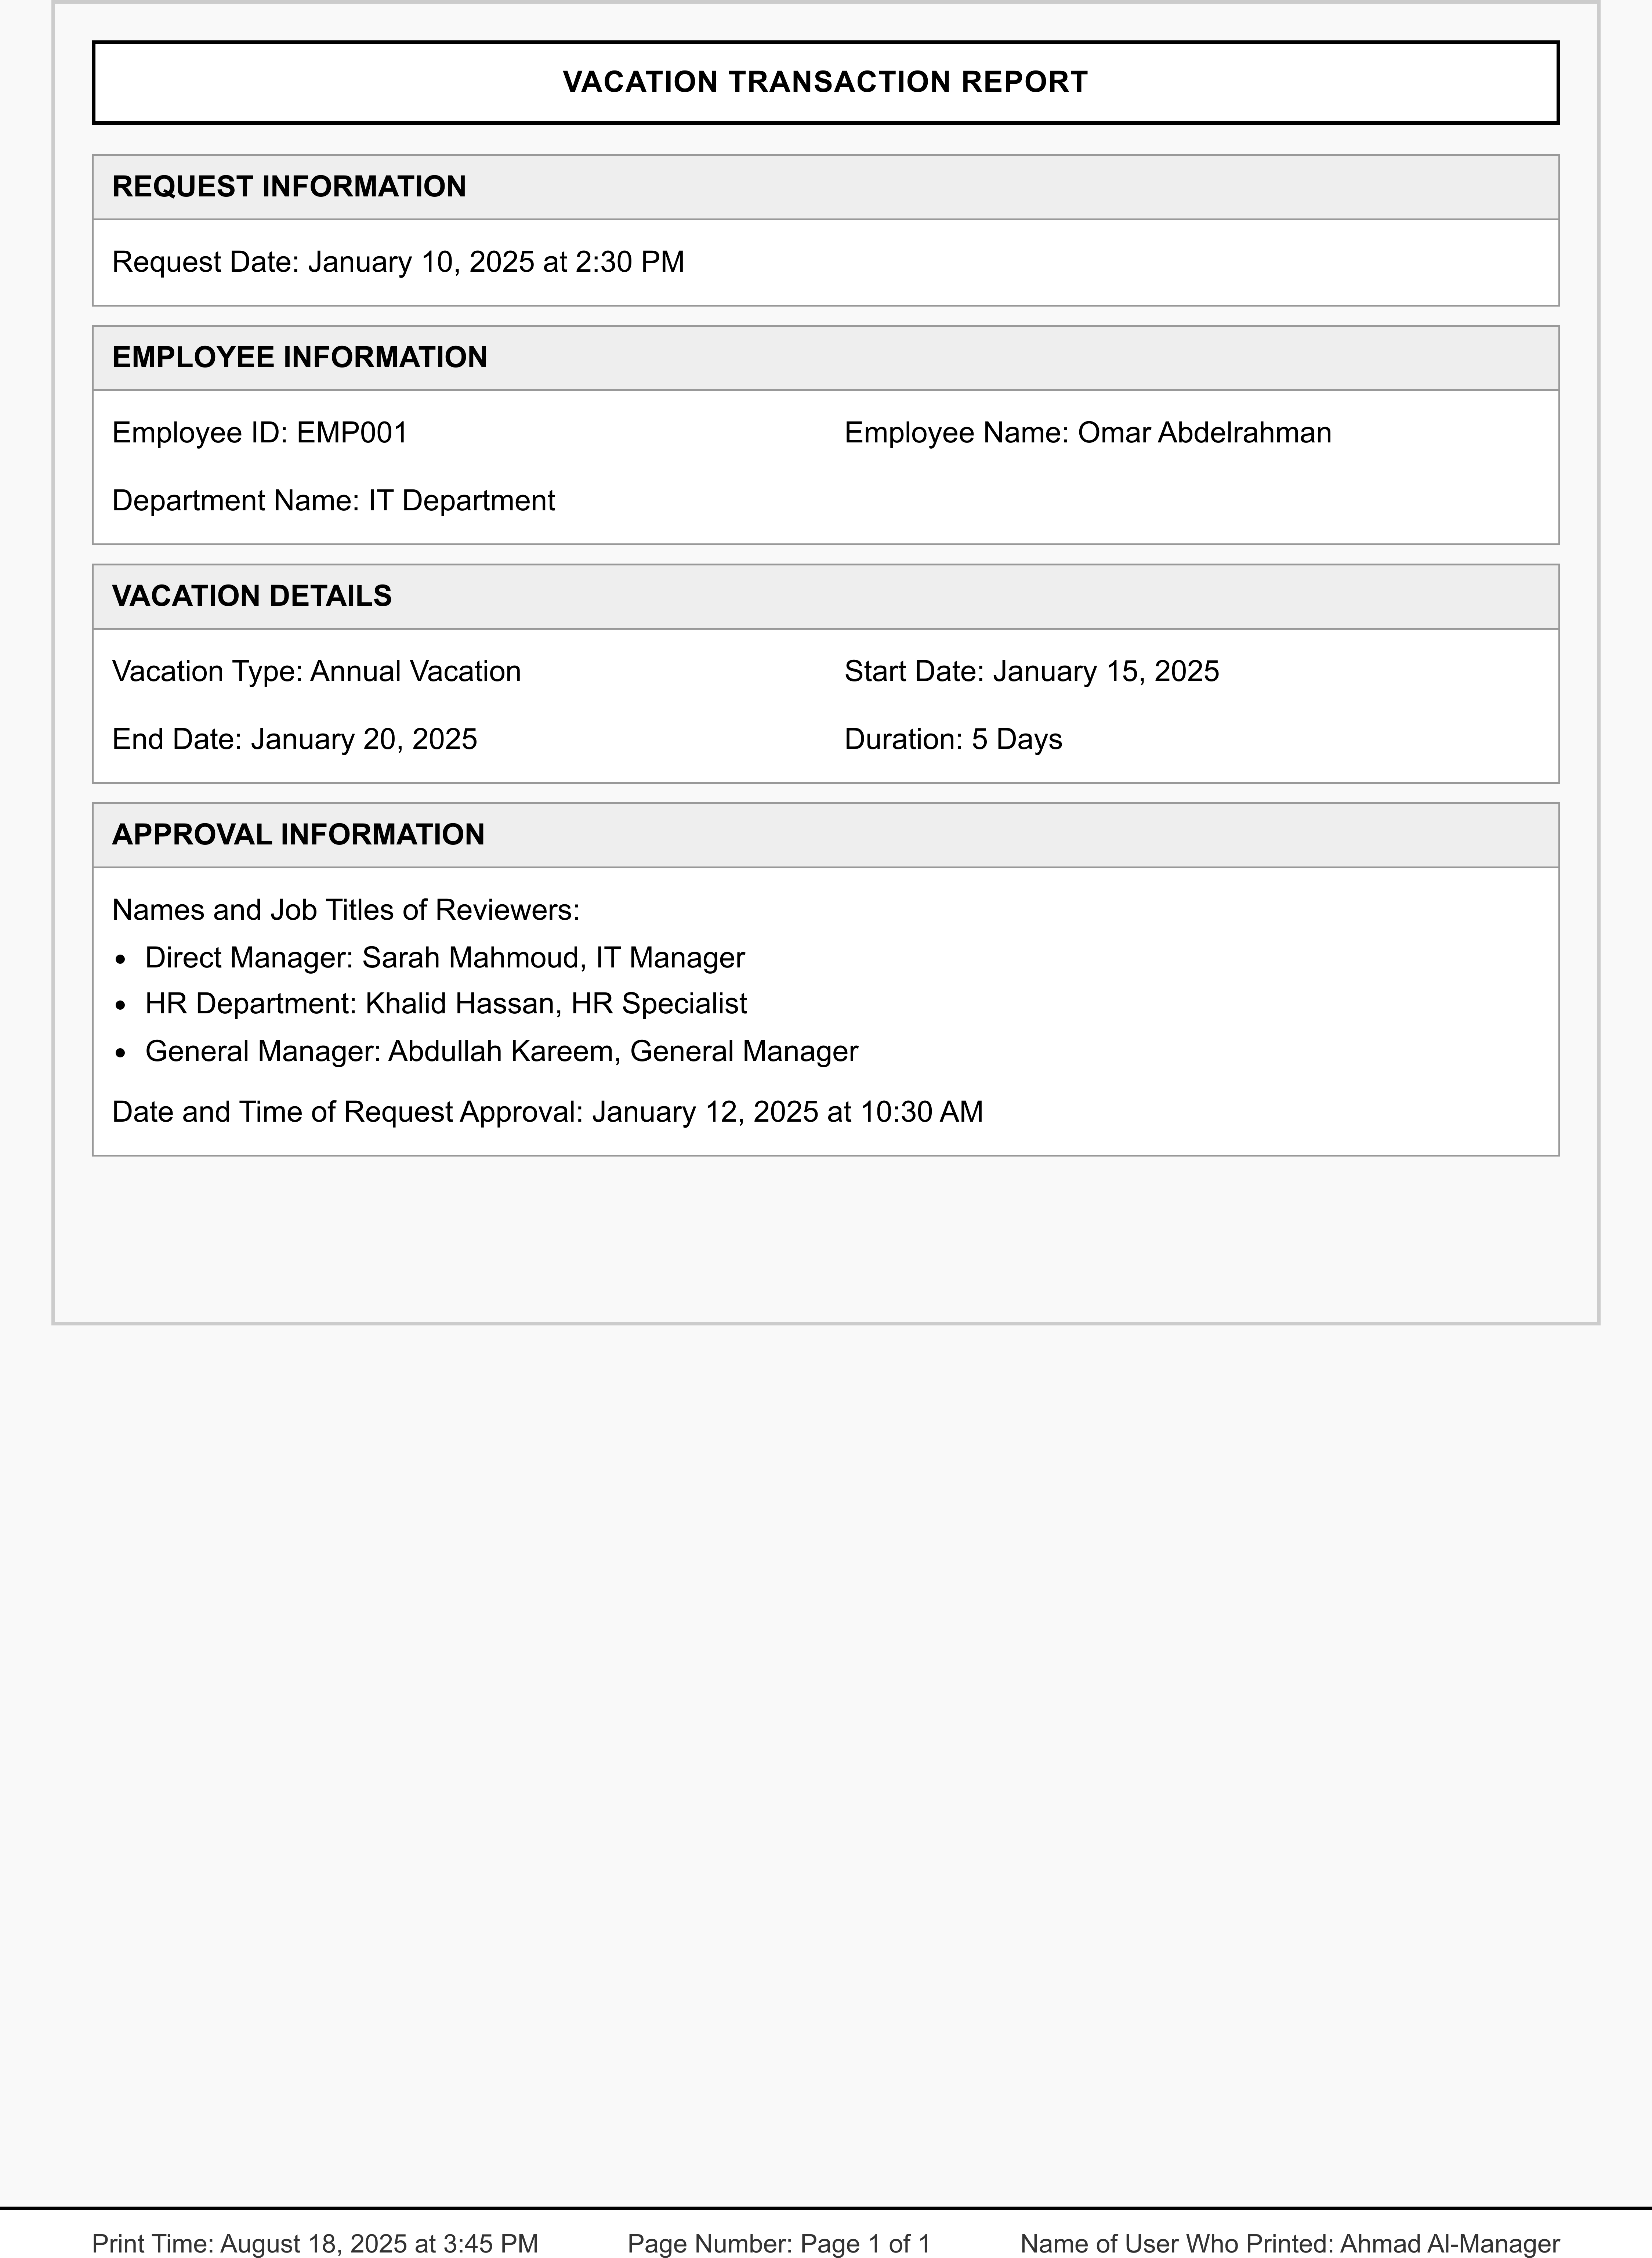
\includegraphics[width=0.8\textwidth]{Wireframes/Print-Layout-Single-Transaction-Report/Print-Layout-Single-Transaction-Report-1.png}
\caption{Single Transaction Report Layout}
\label{fig:single-transaction-report-layout}
\end{figure}

\subsubsection{Annual Comparative Report Layout}
\begin{figure}[H]
\centering
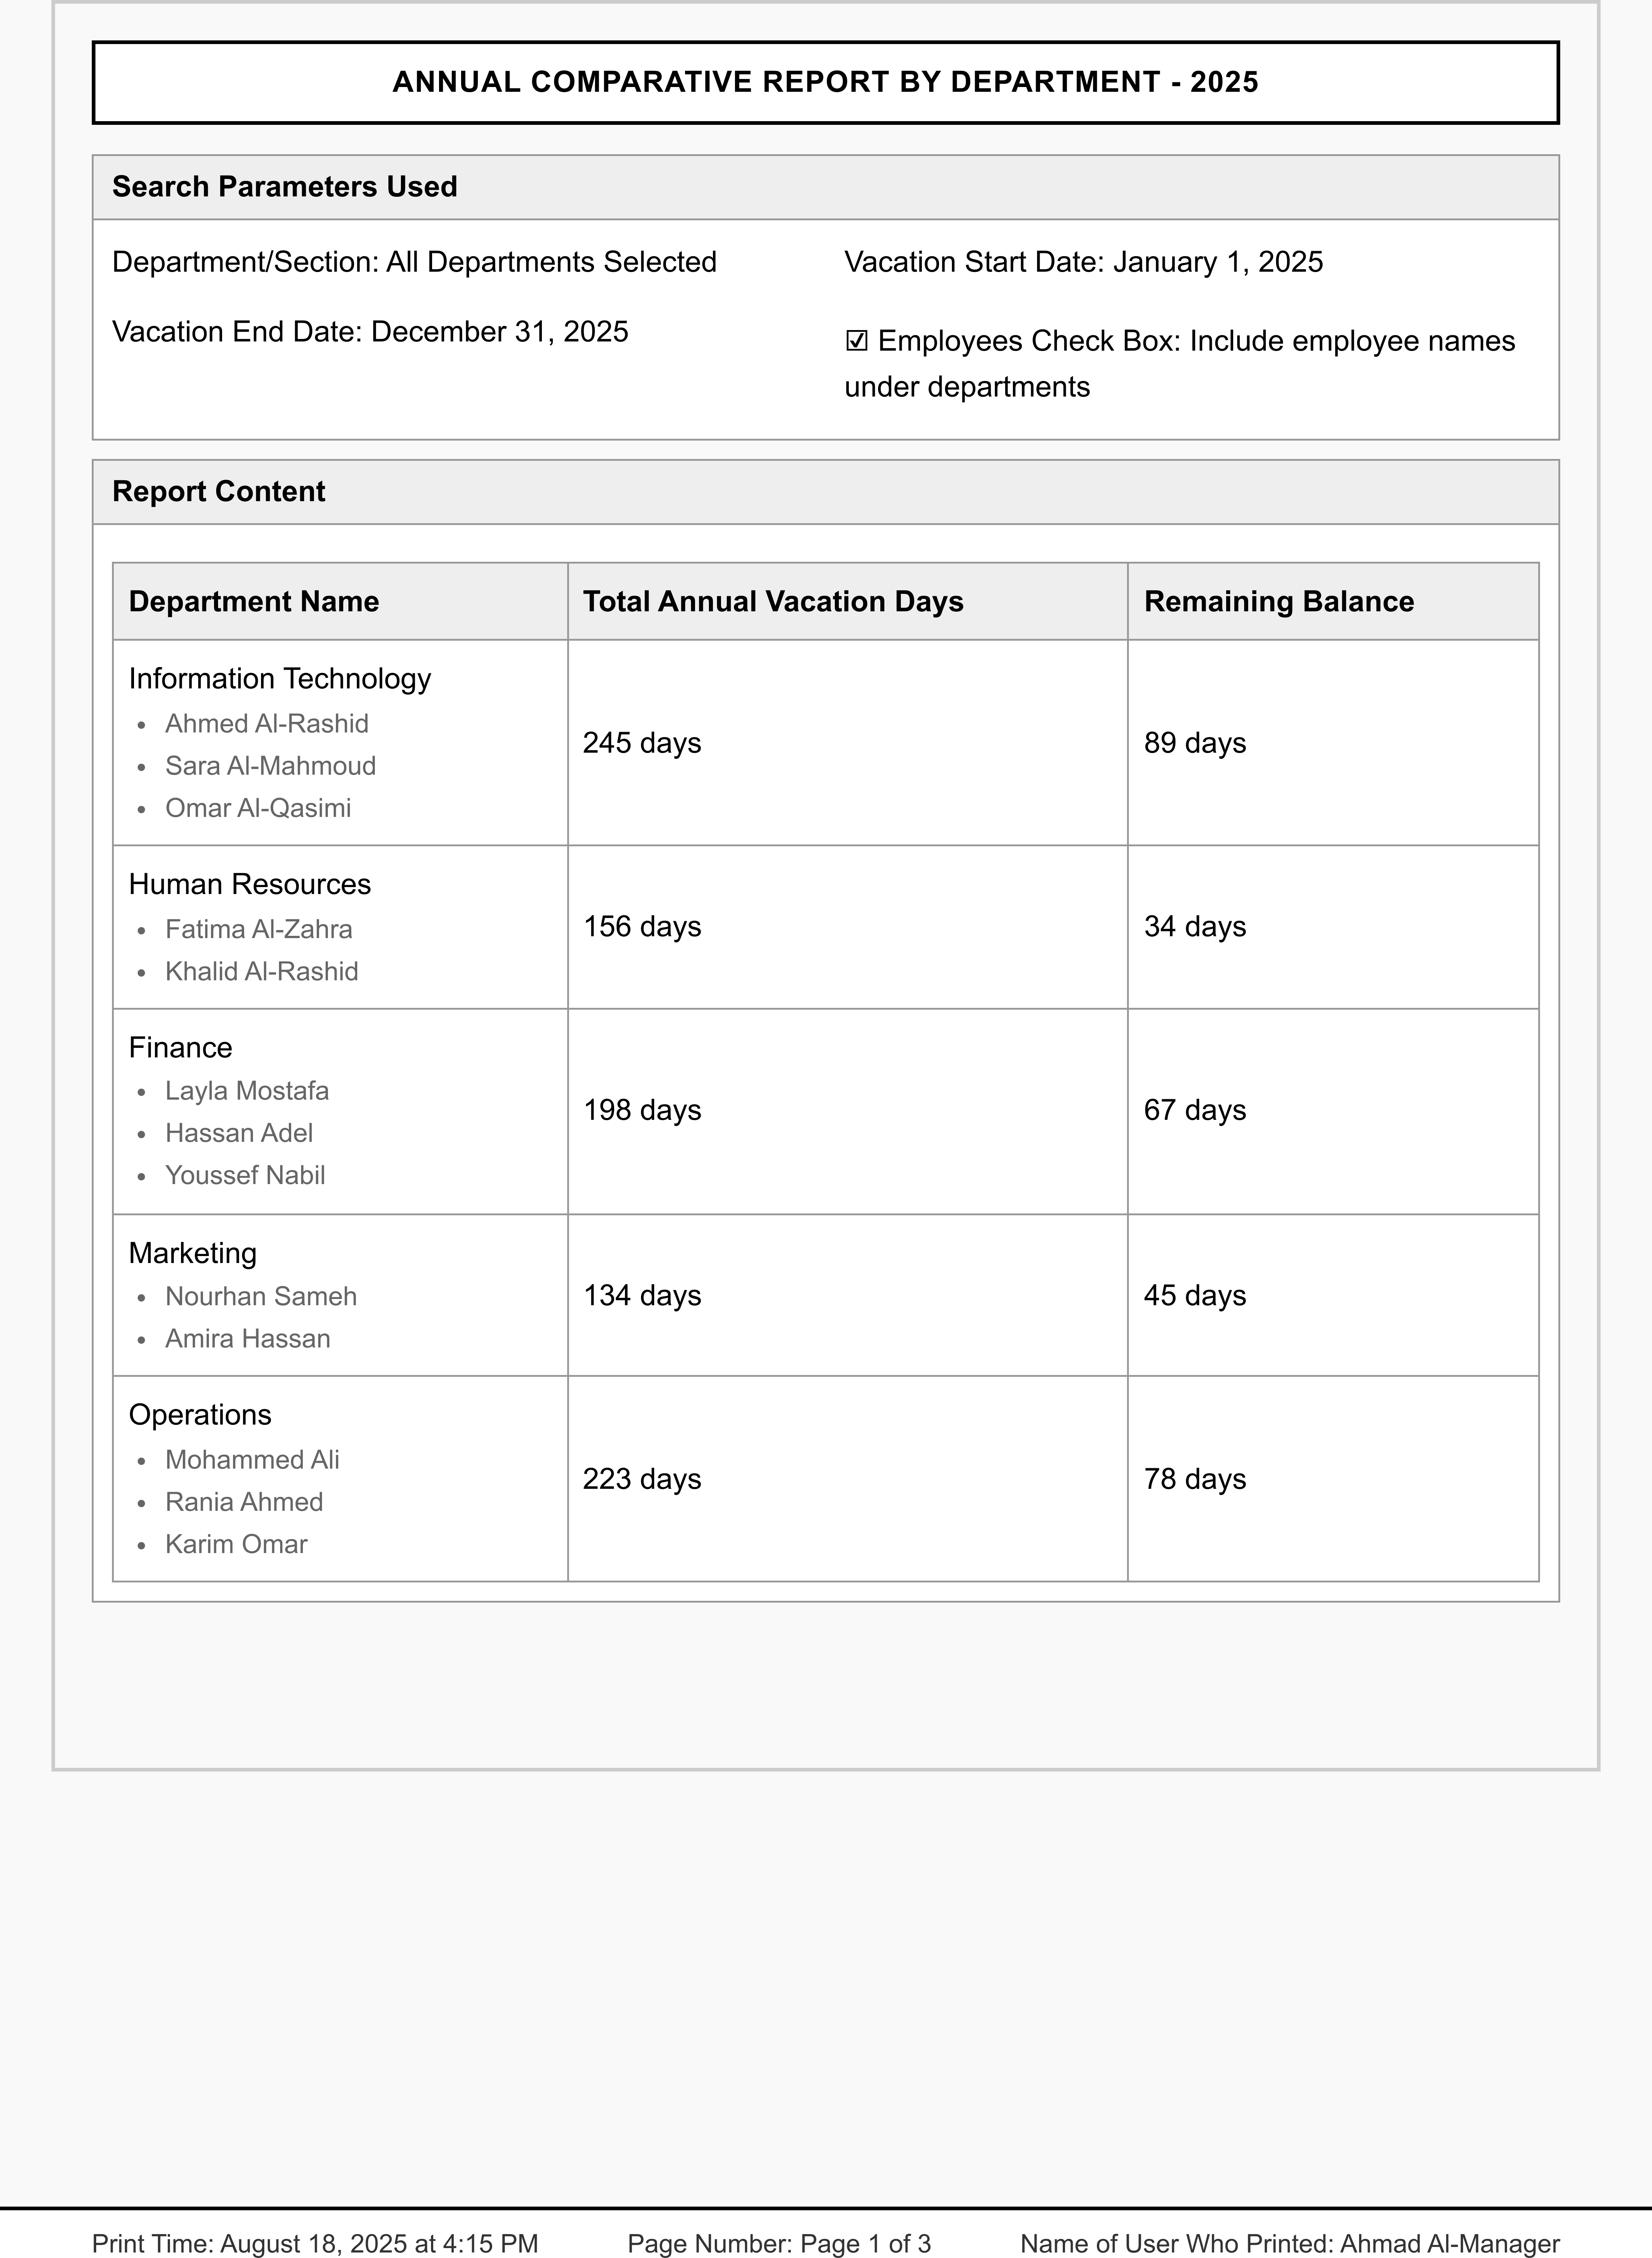
\includegraphics[width=0.8\textwidth]{Wireframes/Print-Layout-Annual-Comparative-Report/Print-Layout-Annual-Comparative-Report-Web-1.png}
\caption{Annual Comparative Report Layout}
\label{fig:annual-comparative-report-layout}
\end{figure}

\subsection{Requests Center}
\begin{figure}[H]
\centering
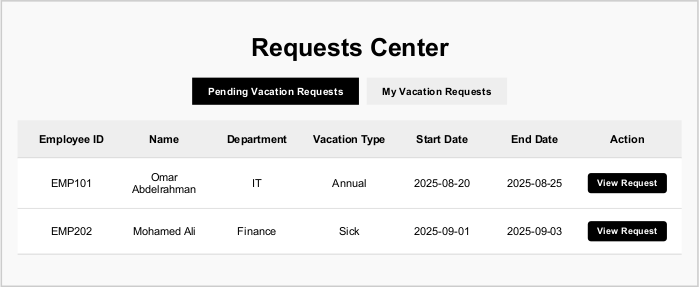
\includegraphics[width=0.8\textwidth]{Wireframes/Requests-Center/Requests-Center-1.png}
\caption{Requests Center Screen}
\label{fig:requests-center-screen}
\end{figure}

\section{Data Requirements and Dictionaries}

The system maintains comprehensive data dictionaries for all entities and screens, ensuring data consistency and proper validation.

\subsection{Master Data Dictionaries}

\subsubsection{Employee Master Data Dictionary}
\begin{figure}[H]
\centering
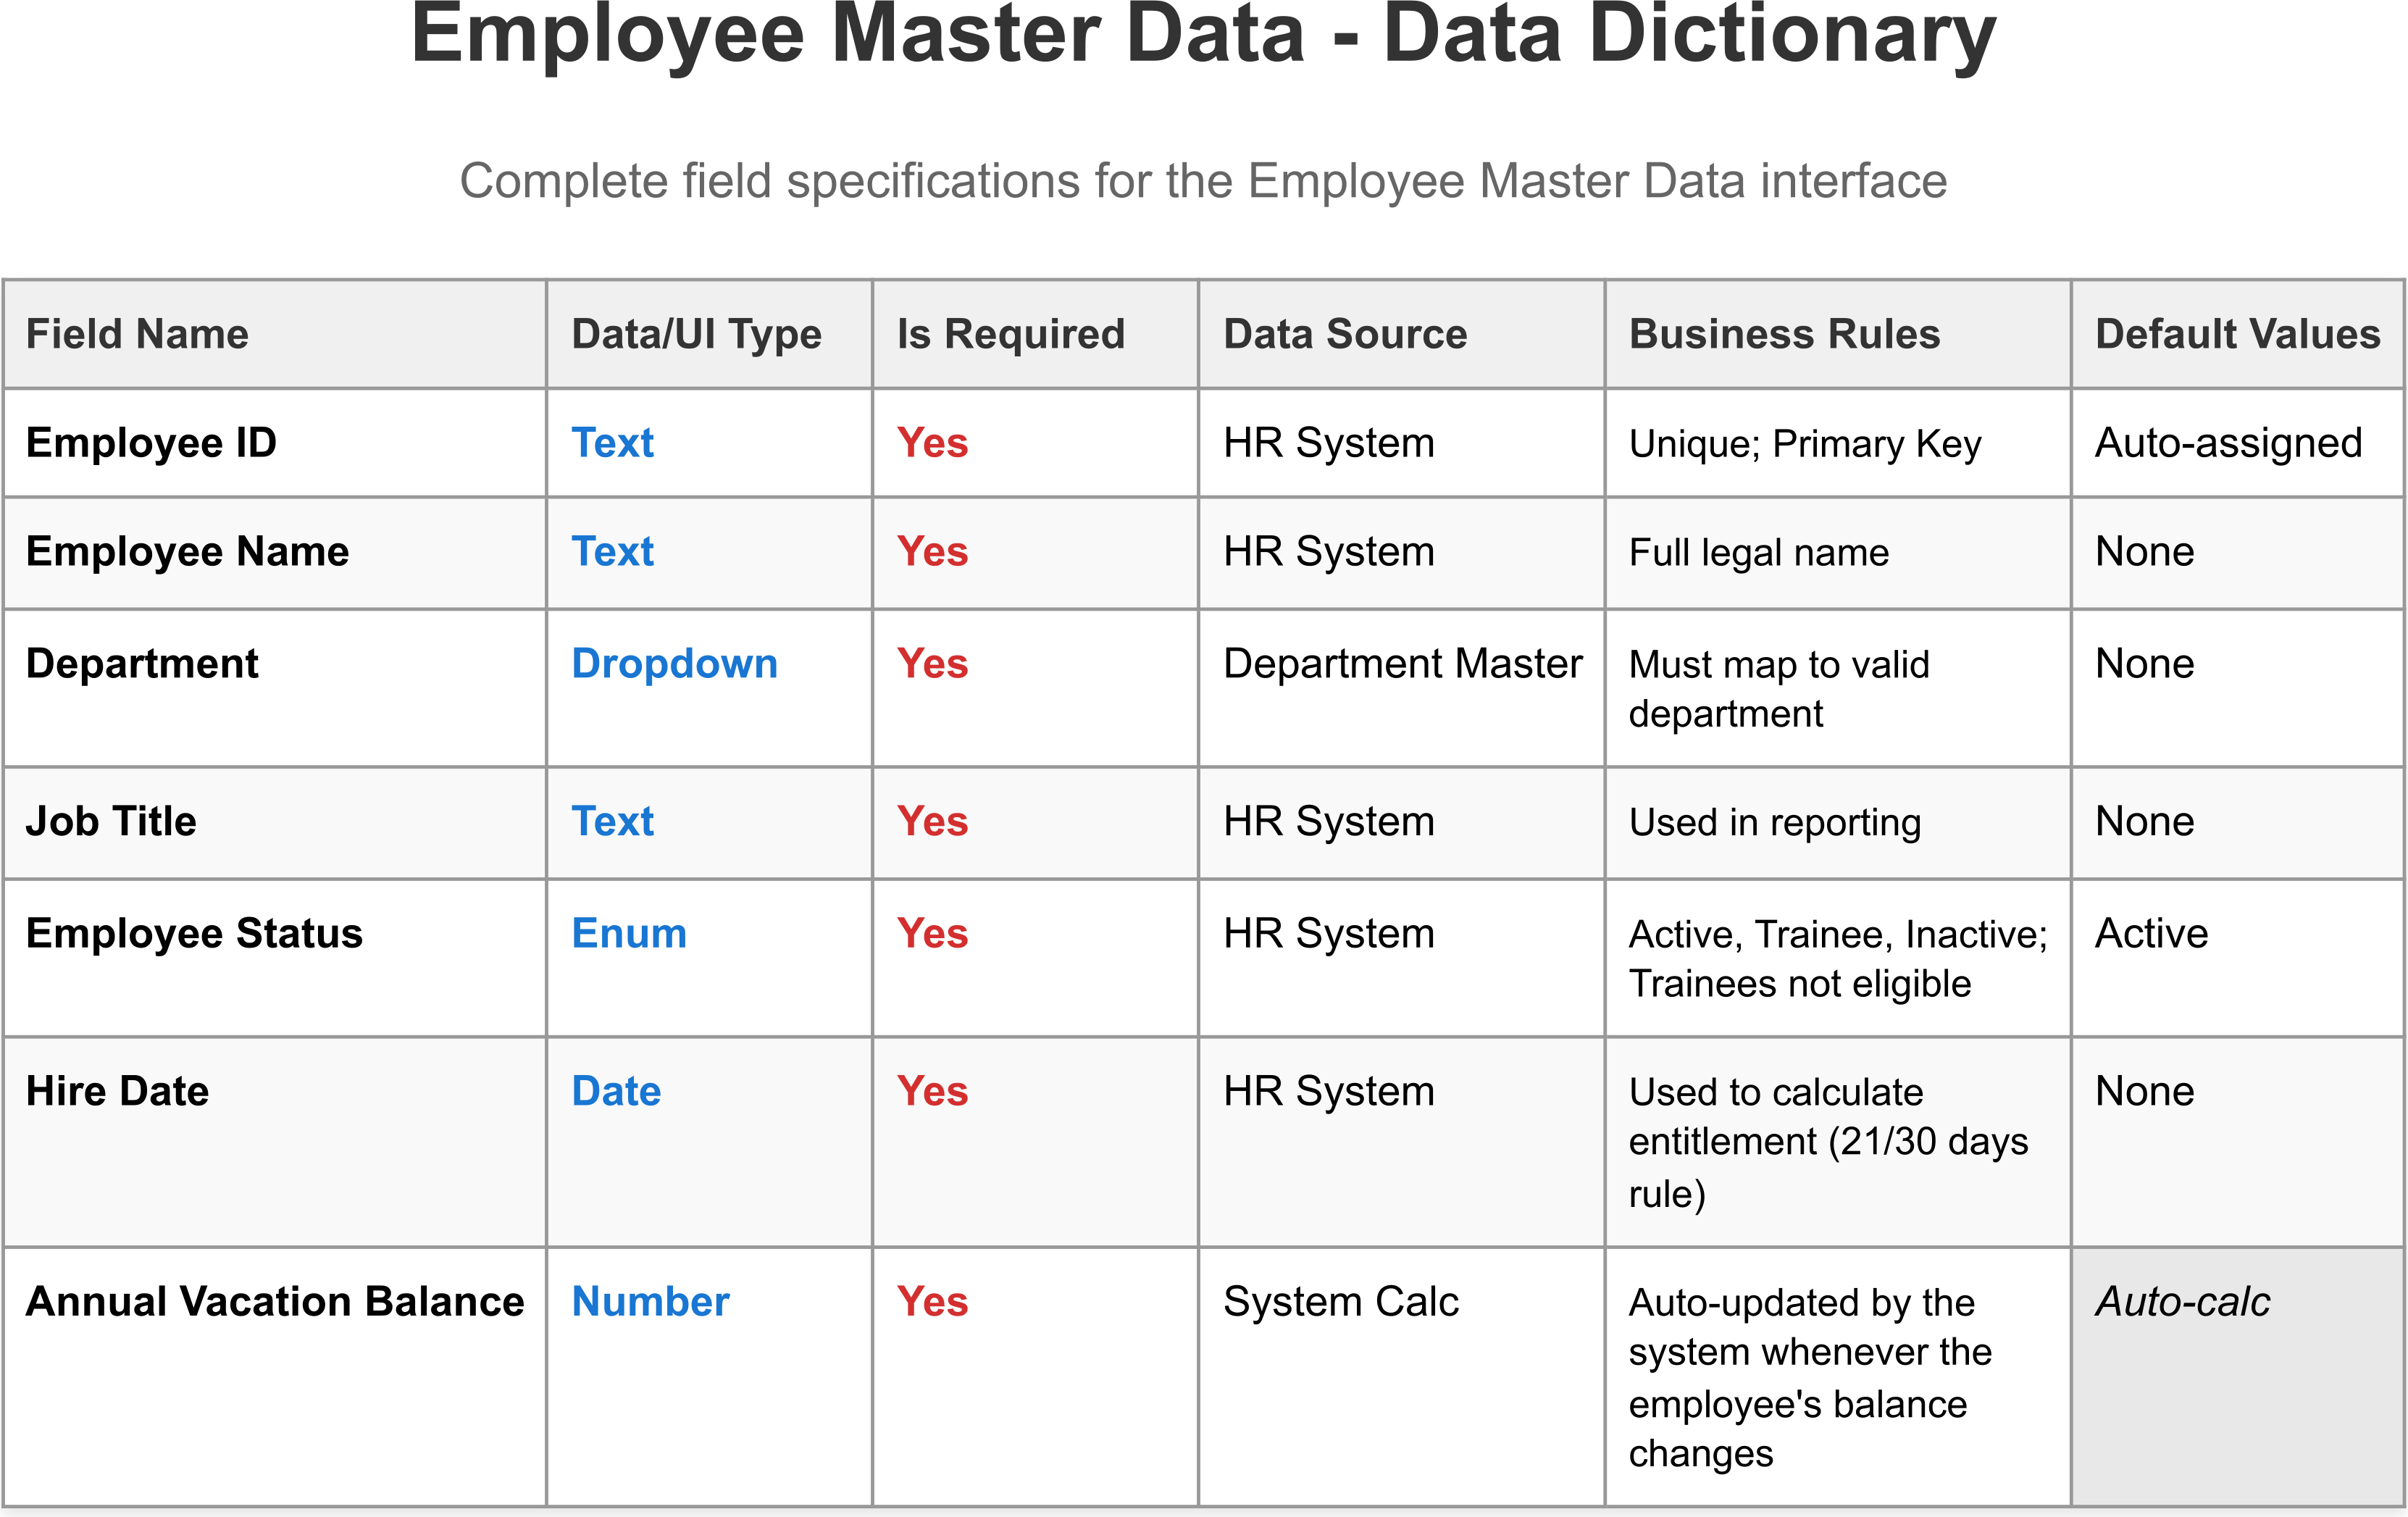
\includegraphics[width=0.8\textwidth]{Data-Dictionary/Master-Data-Dictionaries/Employee-Master-Data-Data-Dictionary/Employee-Master-Data-Data-Dictionary-1.png}
\caption{Employee Master Data Dictionary}
\label{fig:employee-master-data}
\end{figure}

\subsubsection{Departments Master Data Dictionary}
\begin{figure}[H]
\centering
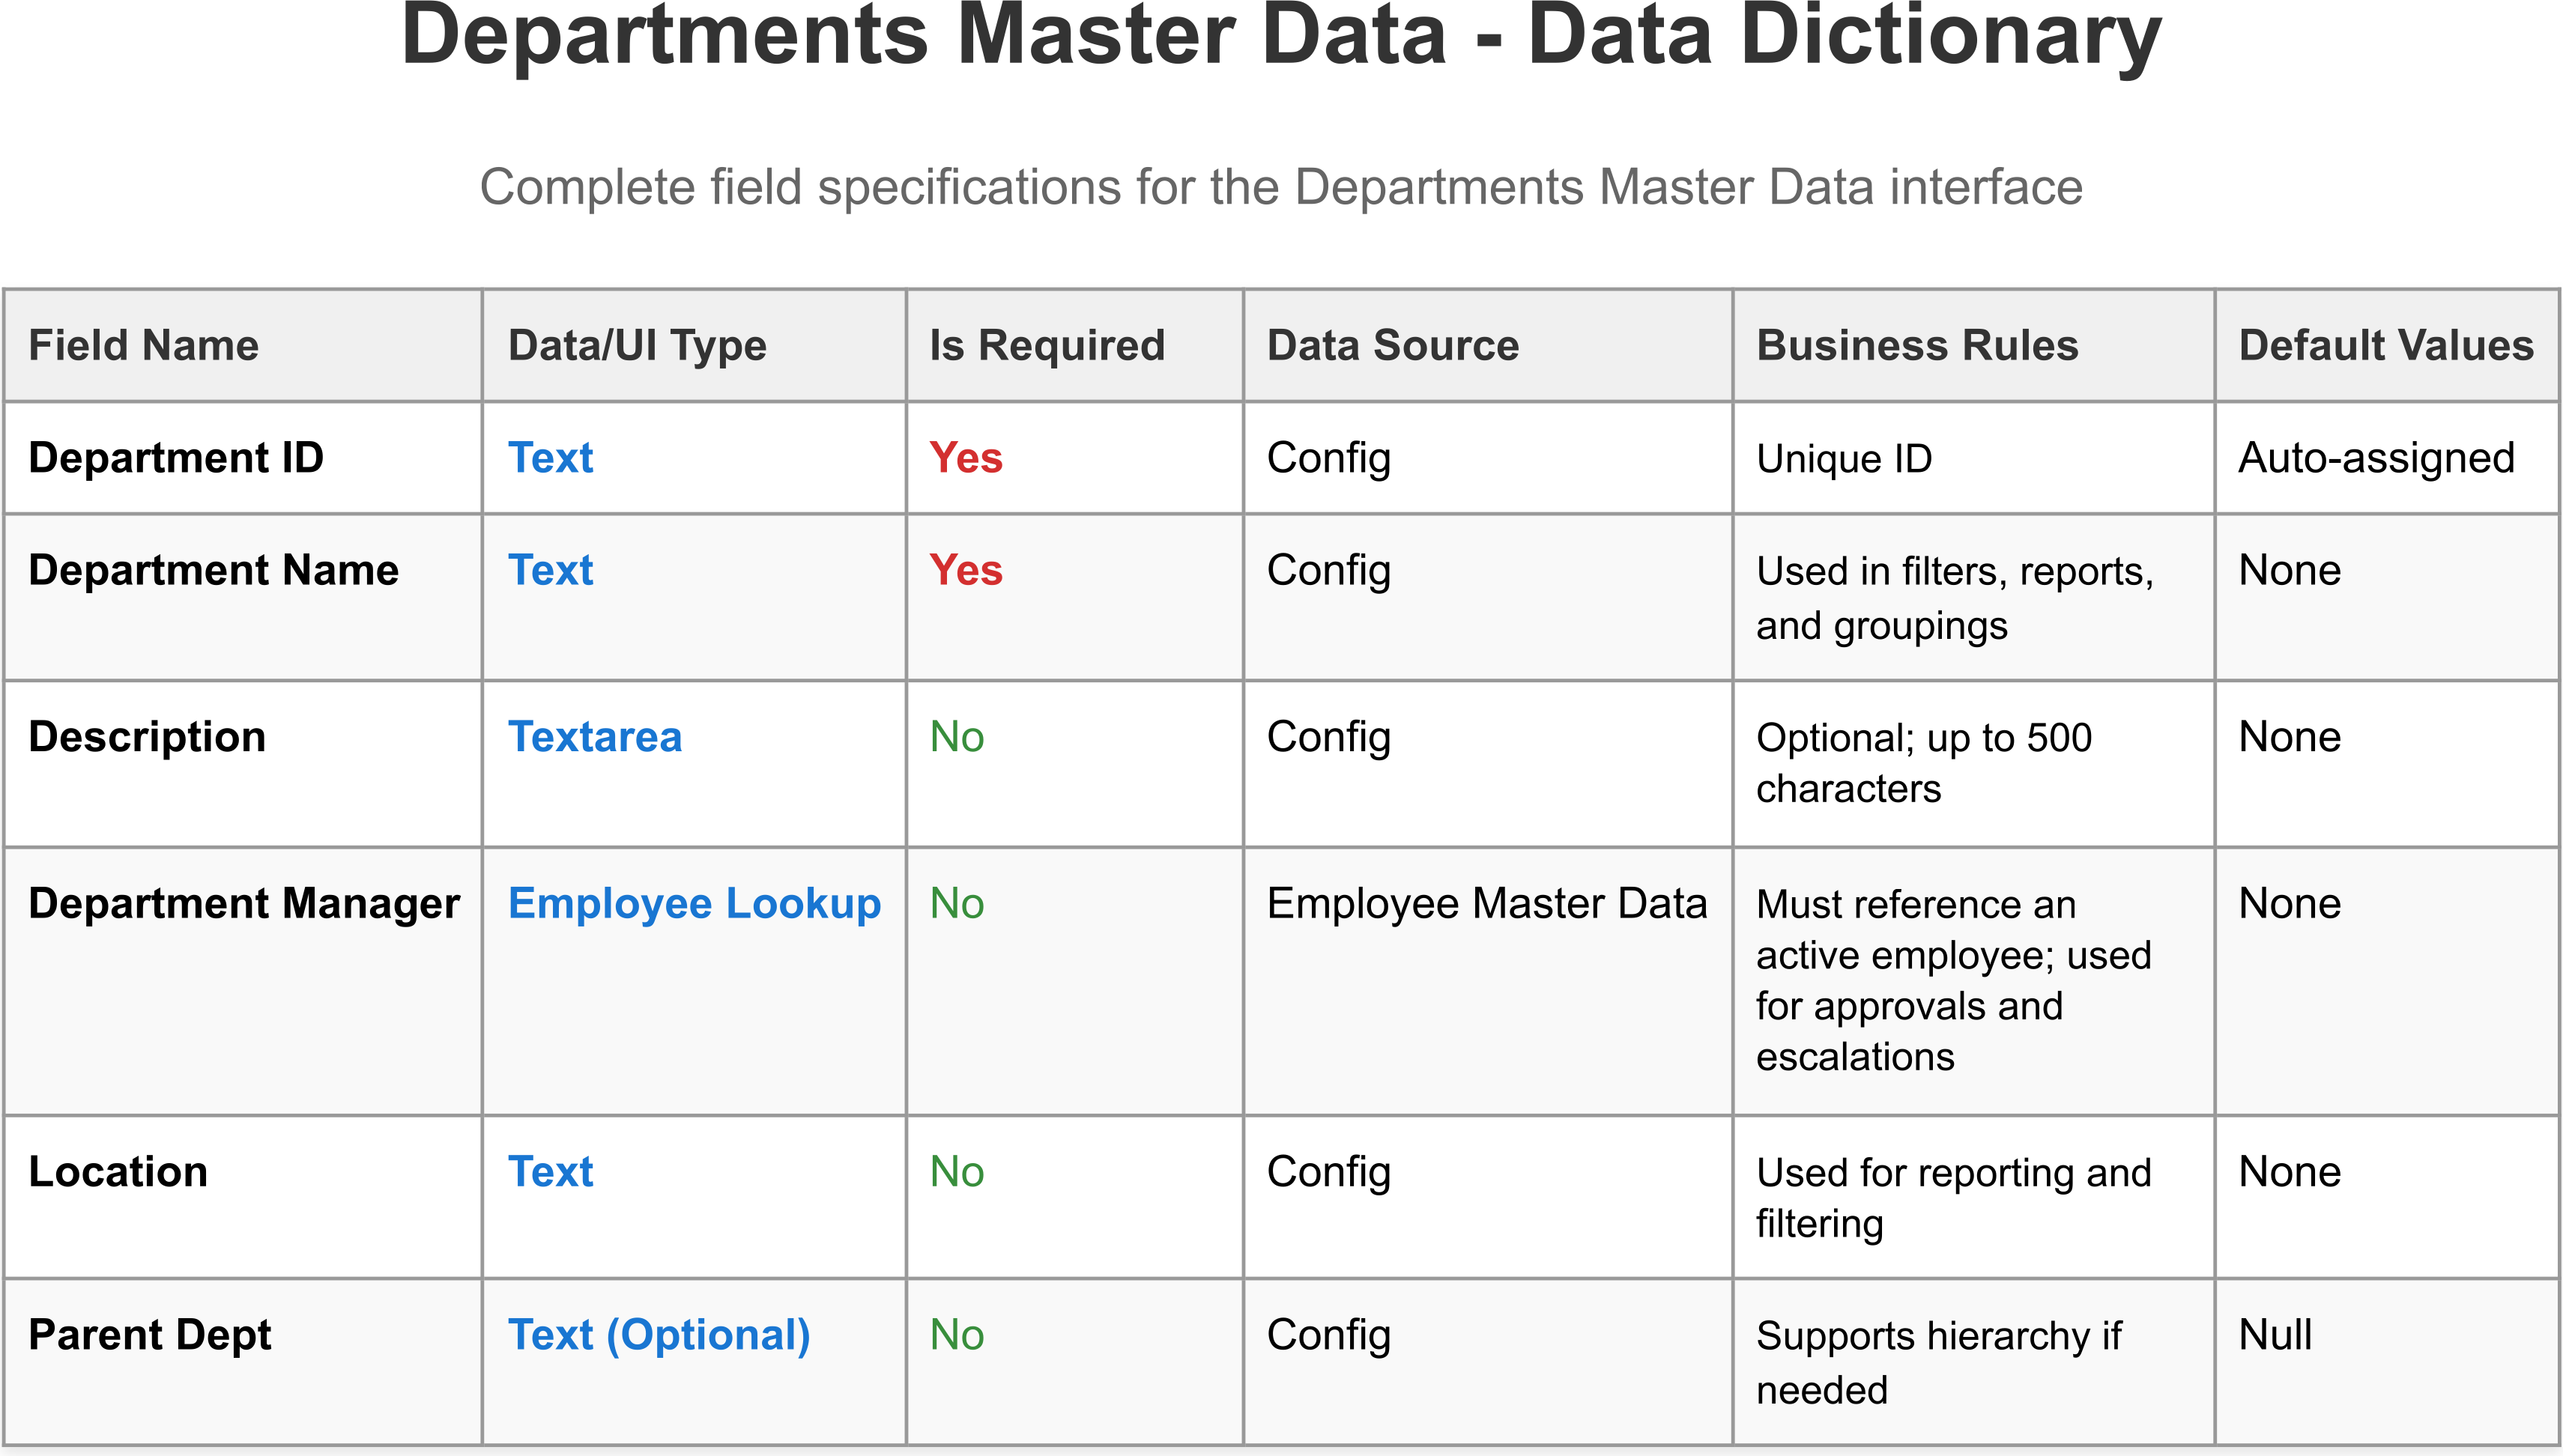
\includegraphics[width=0.8\textwidth]{Data-Dictionary/Master-Data-Dictionaries/Departments-Master-Data-Data-Dictionary/Departments-Master-Data-Data-Dictionary-1.png}
\caption{Departments Master Data Dictionary}
\label{fig:departments-master-data}
\end{figure}

\subsubsection{Vacation Types Master Data Dictionary}
\begin{figure}[H]
\centering
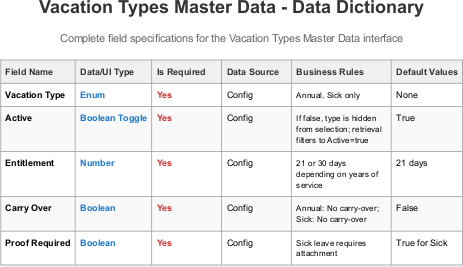
\includegraphics[width=0.8\textwidth]{Data-Dictionary/Master-Data-Dictionaries/Vacation-Types-Master-Data-Data-Dictionary/Vacation-Types-Master-Data-Data-Dictionary-1.png}
\caption{Vacation Types Master Data Dictionary}
\label{fig:vacation-types-master-data}
\end{figure}

\subsection{Screen-Level Data Dictionaries}

\subsubsection{Vacation Request Screen Data Dictionary}
\begin{figure}[H]
\centering
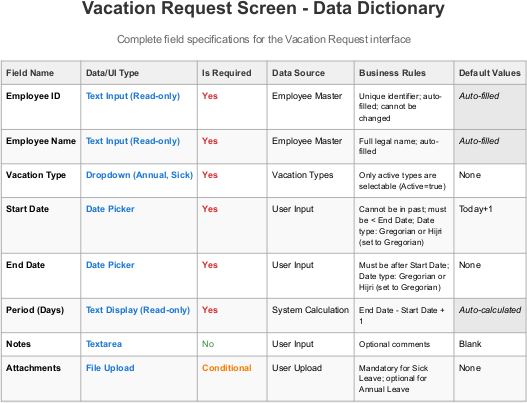
\includegraphics[width=0.8\textwidth]{Data-Dictionary/Screen-Data-Dictionaries/Vacation-Request-Screen-Data-Dictionary/Vacation-Request-Screen-Data-Dictionary-1.png}
\caption{Vacation Request Screen Data Dictionary}
\label{fig:vacation-request-data-dict}
\end{figure}

\subsubsection{Vacation Cancellation Request Screen Data Dictionary}
\begin{figure}[H]
\centering
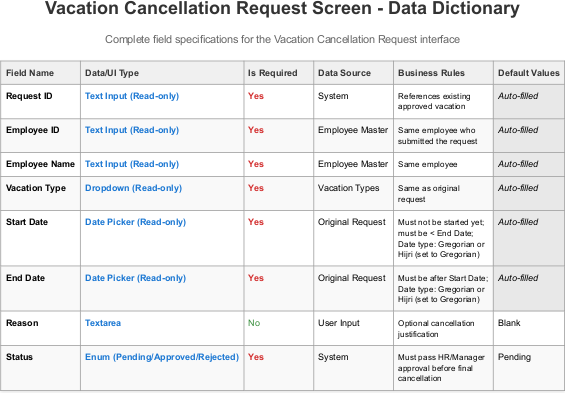
\includegraphics[width=0.8\textwidth]{Data-Dictionary/Screen-Data-Dictionaries/Vacation-Cancellation-Request-Screen-Data-Dictionary/Vacation-Cancellation-Request-Screen-Data-Dictionary-1.png}
\caption{Vacation Cancellation Request Screen Data Dictionary}
\label{fig:vacation-cancellation-data-dict}
\end{figure}

\subsubsection{Review Vacation Request Screen Data Dictionary}
\begin{figure}[H]
\centering
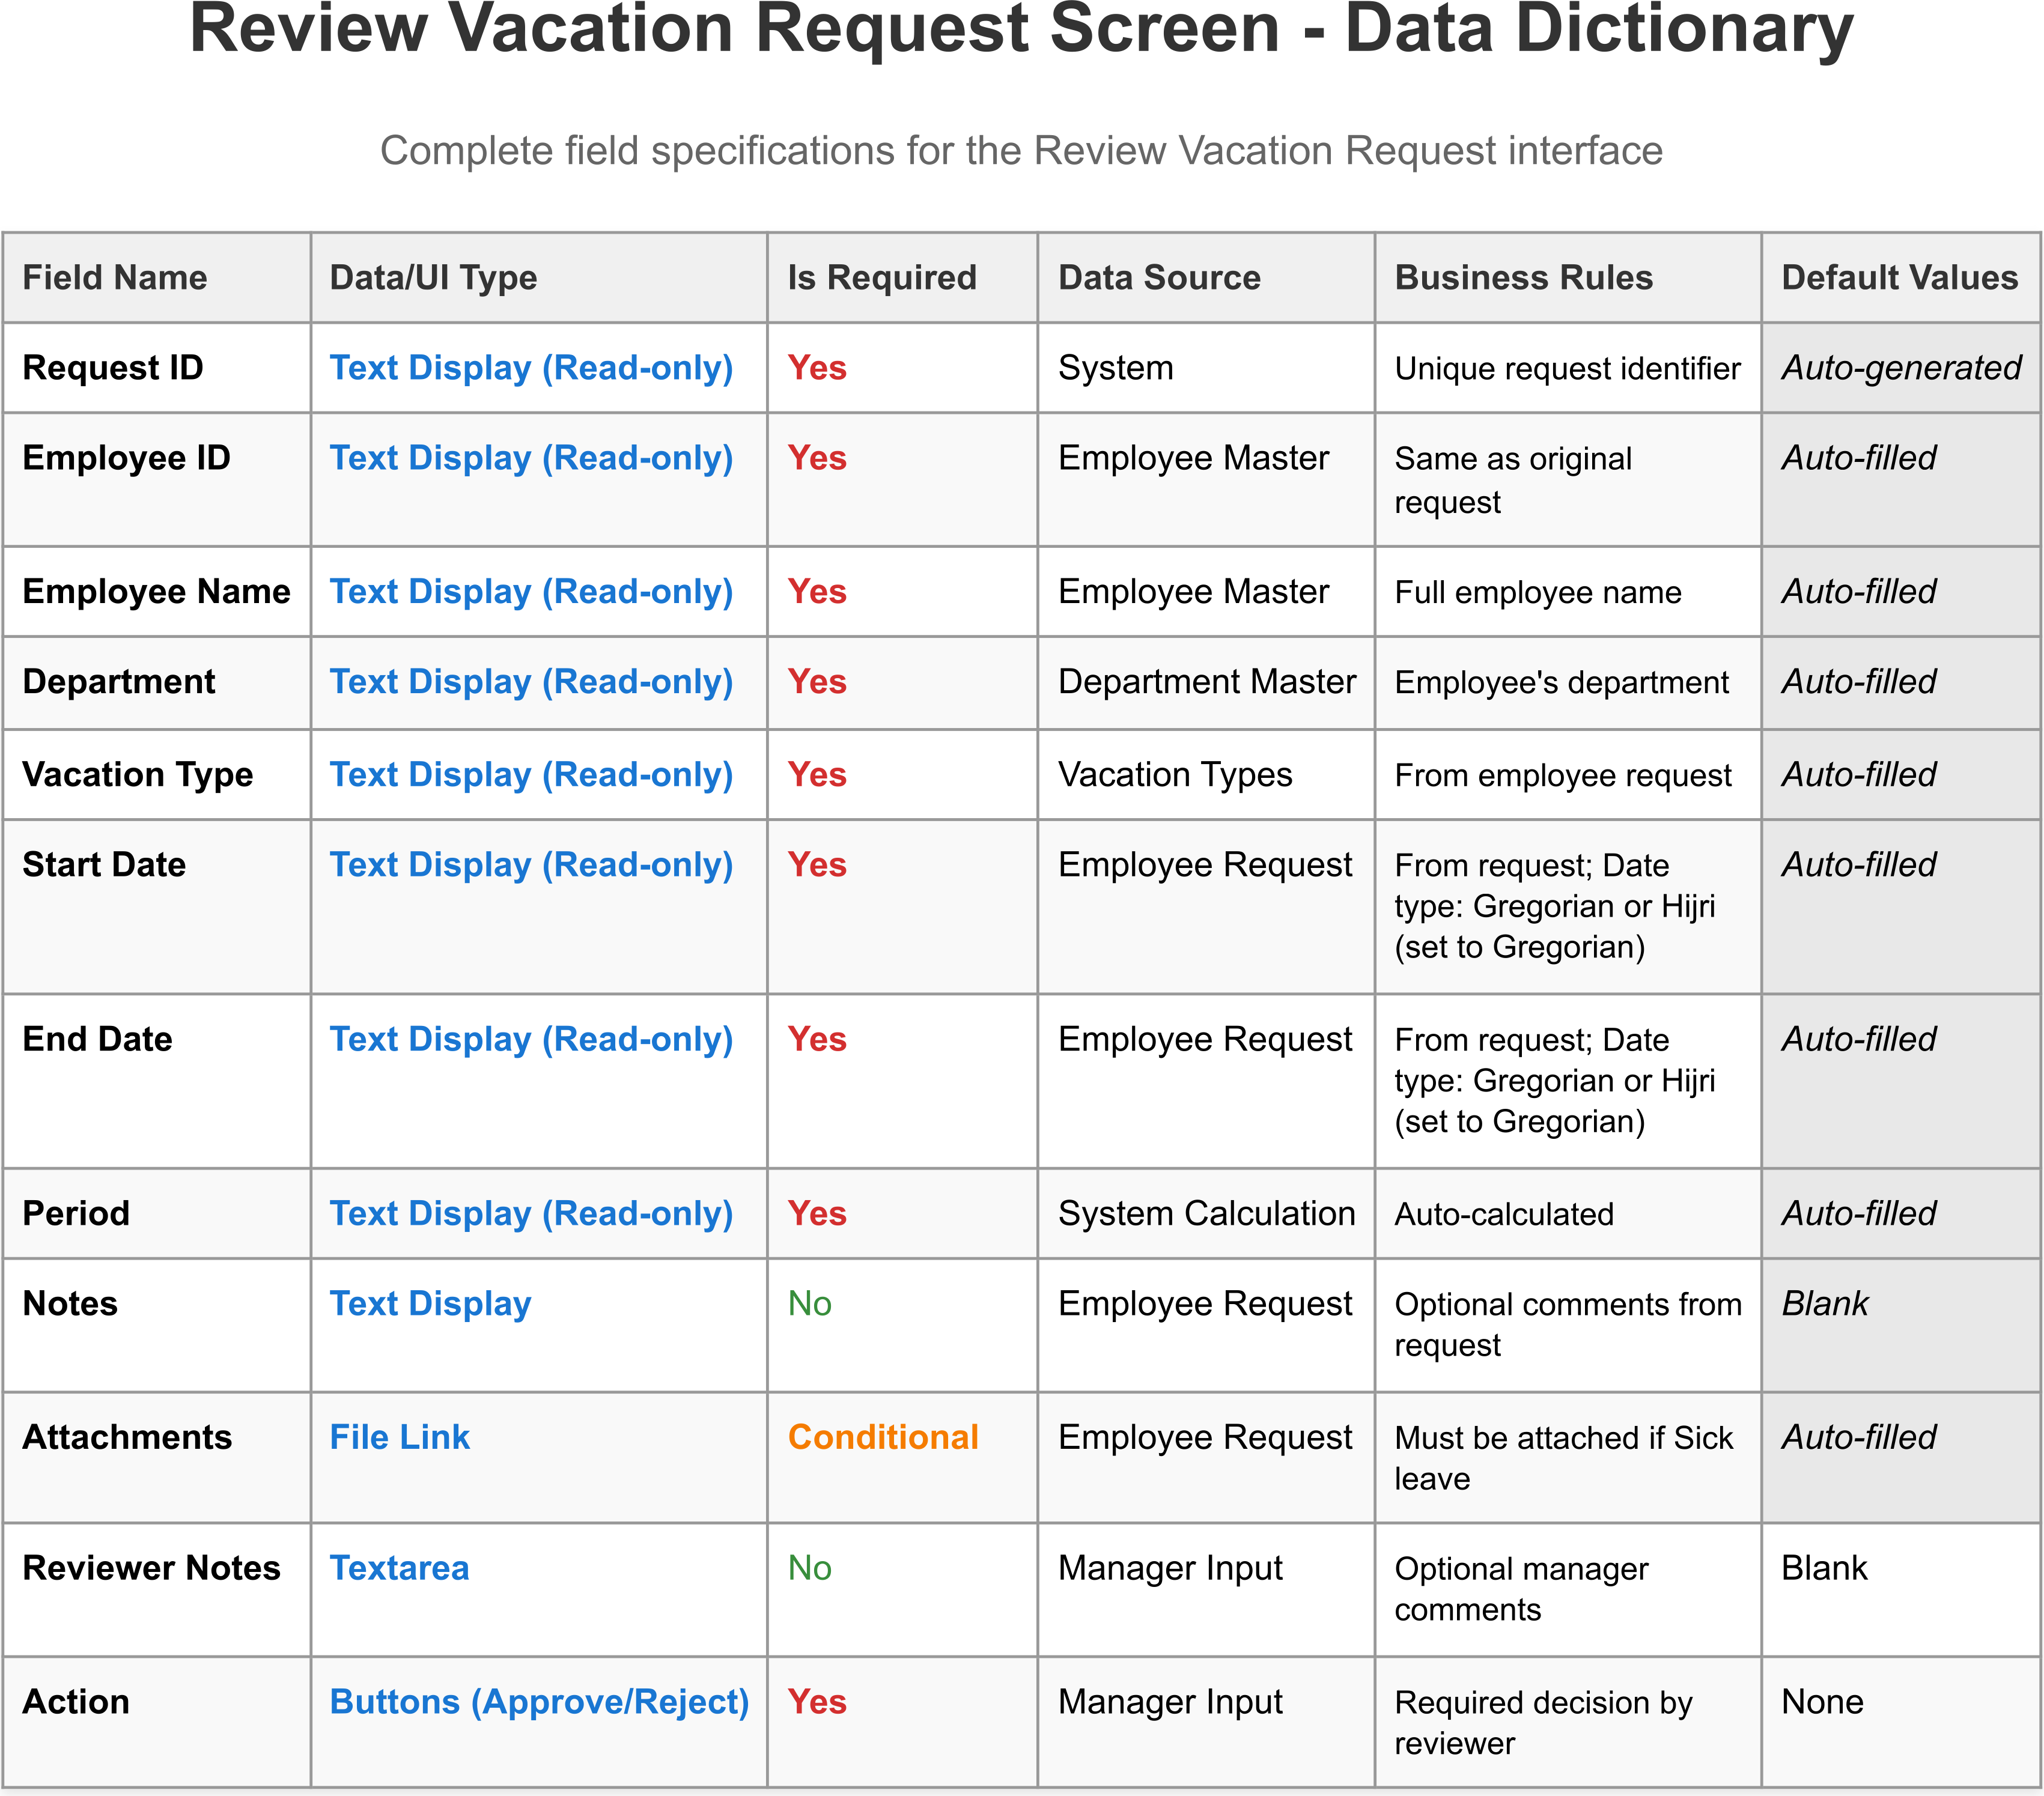
\includegraphics[width=0.8\textwidth]{Data-Dictionary/Screen-Data-Dictionaries/Review-Vacation-Request-Screen-Data-Dictionary/Review-Vacation-Request-Screen-Data-Dictionary-1.png}
\caption{Review Vacation Request Screen Data Dictionary}
\label{fig:review-vacation-data-dict}
\end{figure}

\subsubsection{Review Vacation Cancellation Request Screen Data Dictionary}
\begin{figure}[H]
\centering
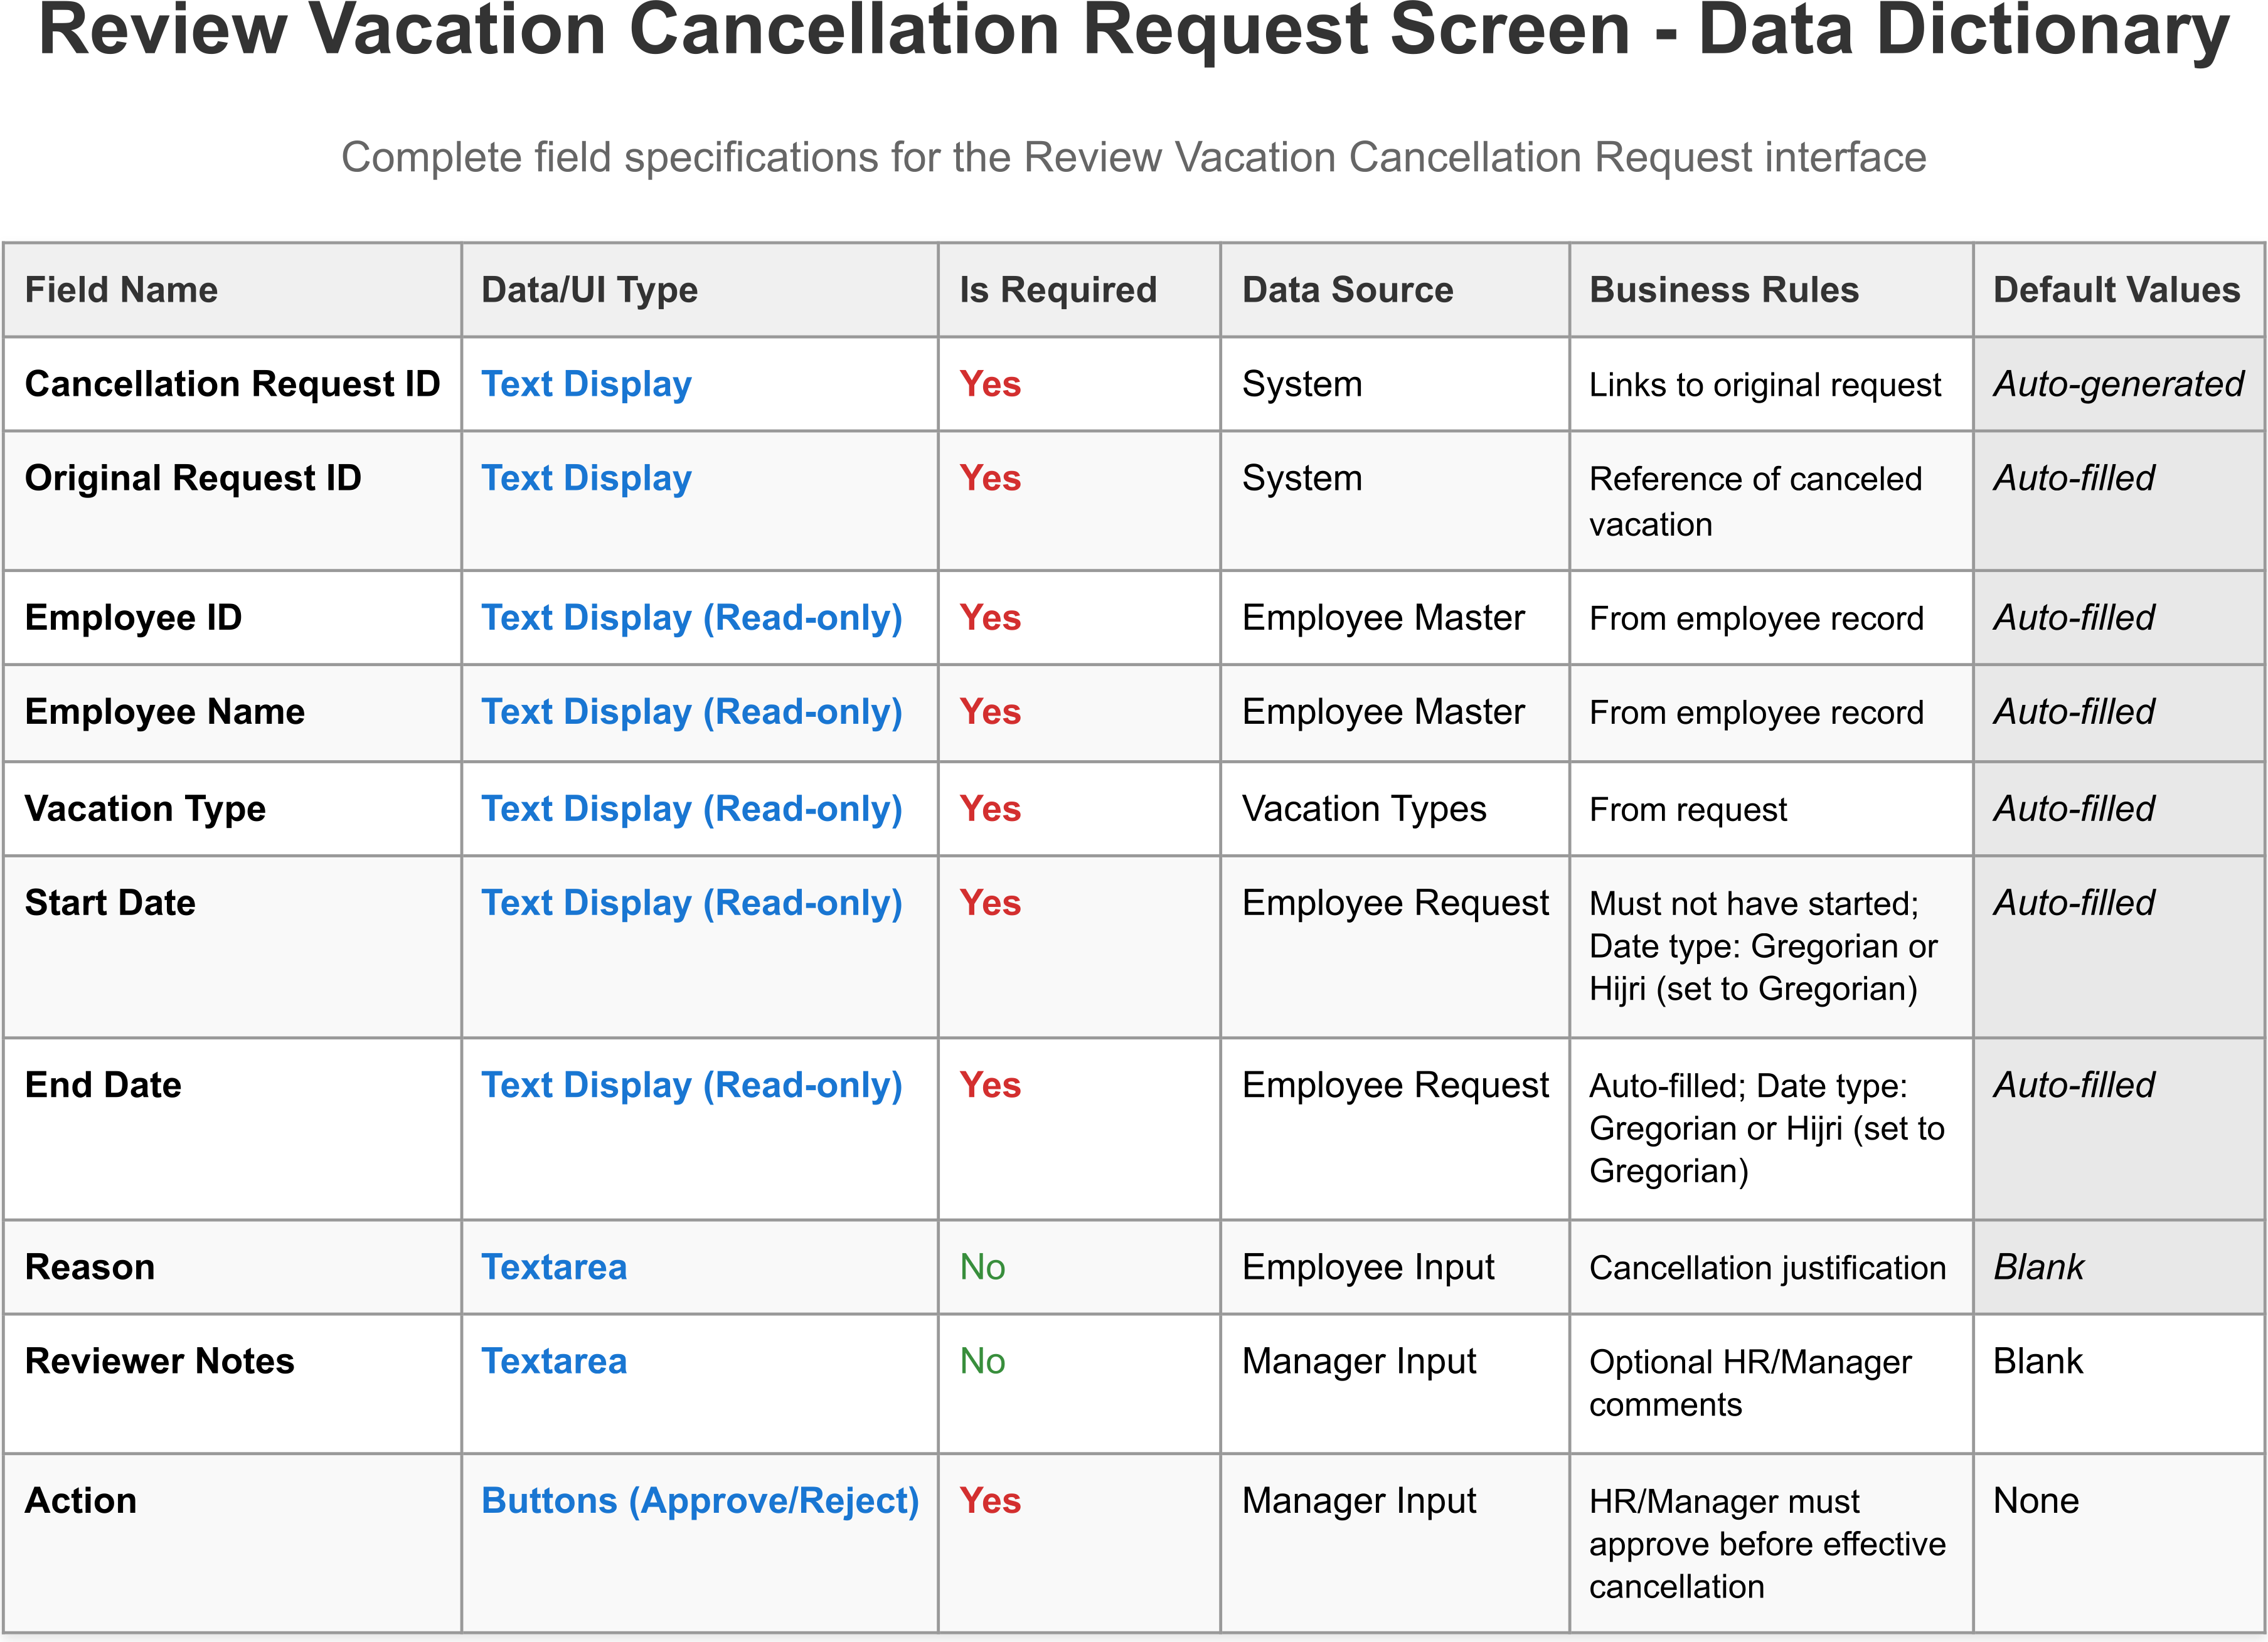
\includegraphics[width=0.8\textwidth]{Data-Dictionary/Screen-Data-Dictionaries/Review-Vacation-Cancellation-Request-Screen-Data-Dictionary/Review-Vacation-Cancellation-Request-Screen-Data-Dictionary-1.png}
\caption{Review Vacation Cancellation Request Screen Data Dictionary}
\label{fig:review-cancellation-data-dict}
\end{figure}

\subsubsection{My Vacation Requests Screen Data Dictionary}
\begin{figure}[H]
\centering
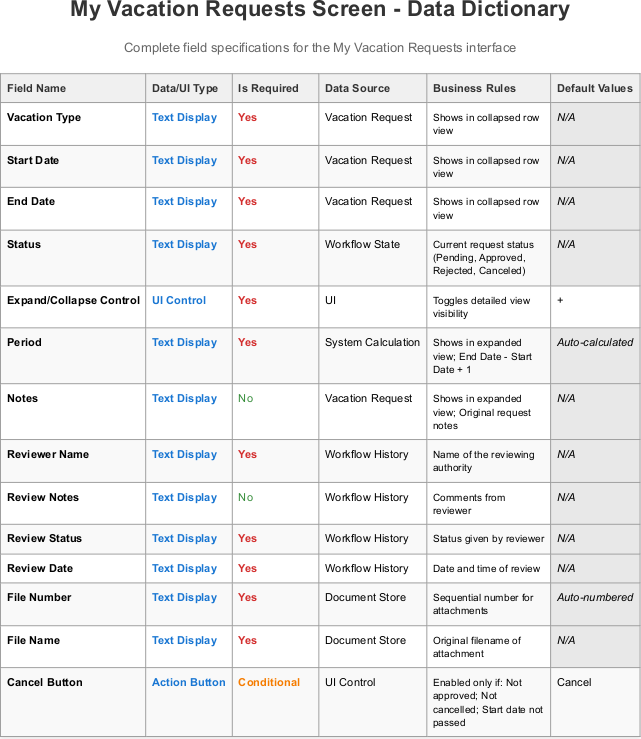
\includegraphics[width=0.8\textwidth]{Data-Dictionary/Screen-Data-Dictionaries/My-Vacation-Requests-Screen-Data-Dictionary/My-Vacation-Requests-Screen-Data-Dictionary-1.png}
\caption{My Vacation Requests Screen Data Dictionary}
\label{fig:my-vacation-requests-data-dict}
\end{figure}

\subsubsection{Pending Vacation Requests Screen Data Dictionary}
\begin{figure}[H]
\centering
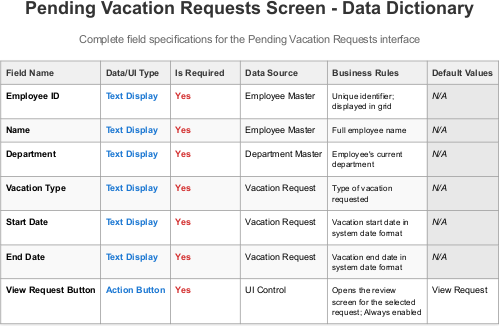
\includegraphics[width=0.8\textwidth]{Data-Dictionary/Screen-Data-Dictionaries/Pending-Vacation-Requests-Screen-Data-Dictionary/Pending-Vacation-Requests-Screen-Data-Dictionary-1.png}
\caption{Pending Vacation Requests Screen Data Dictionary}
\label{fig:pending-vacation-requests-data-dict}
\end{figure}

\subsubsection{Vacation Inquiry Search Parameters Screen Data Dictionary}
\begin{figure}[H]
\centering
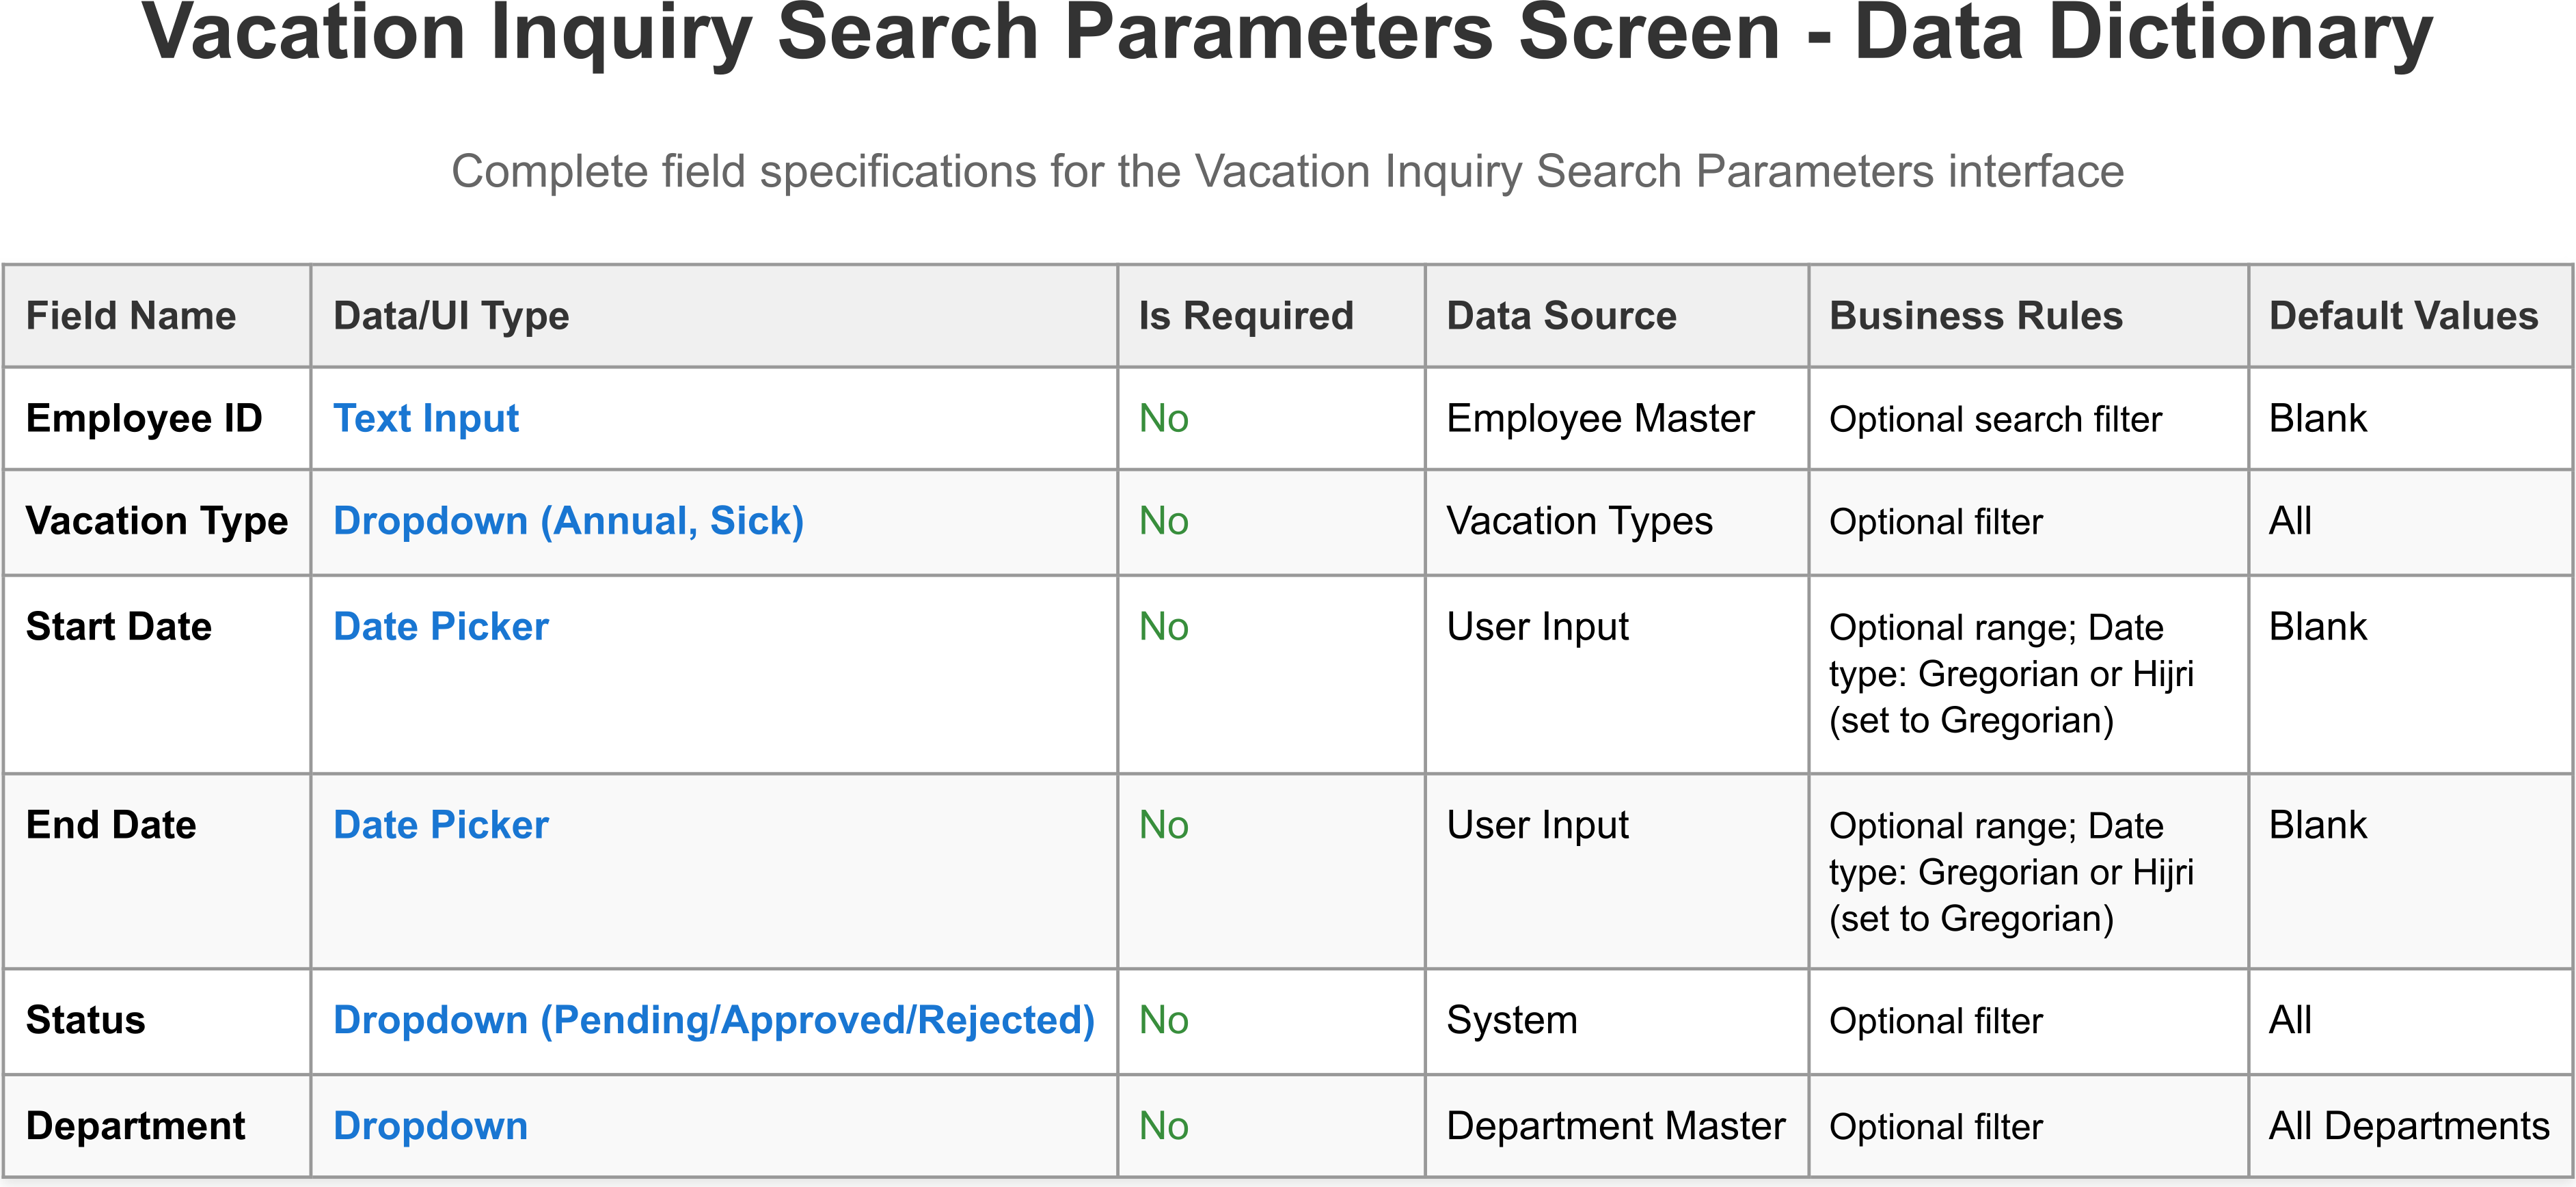
\includegraphics[width=0.8\textwidth]{Data-Dictionary/Screen-Data-Dictionaries/Vacation-Inquiry-Search-Parameters-Screen-Data-Dictionary/Vacation-Inquiry-Search-Parameters-Screen-Data-Dictionary-1.png}
\caption{Vacation Inquiry Search Parameters Screen Data Dictionary}
\label{fig:inquiry-search-params-data-dict}
\end{figure}

\subsubsection{Vacation Inquiry Search Results Screen Data Dictionary}
\begin{figure}[H]
\centering
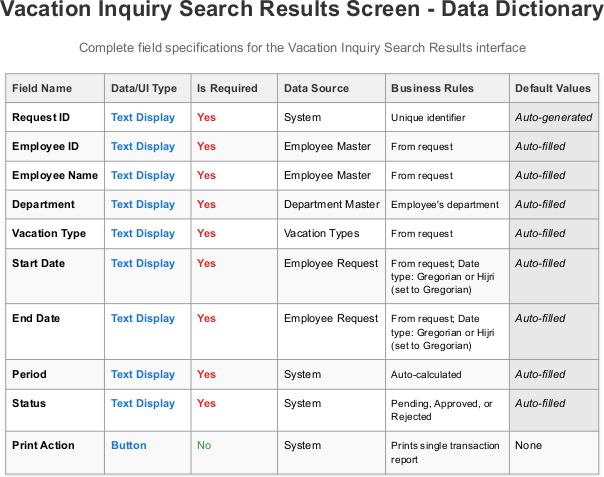
\includegraphics[width=0.8\textwidth]{Data-Dictionary/Screen-Data-Dictionaries/Vacation-Inquiry-Search-Results-Screen-Data-Dictionary/Vacation-Inquiry-Search-Results-Screen-Data-Dictionary-1.png}
\caption{Vacation Inquiry Search Results Screen Data Dictionary}
\label{fig:inquiry-search-results-data-dict}
\end{figure}

\subsubsection{Notifications Center Screen Data Dictionary}
\begin{figure}[H]
\centering
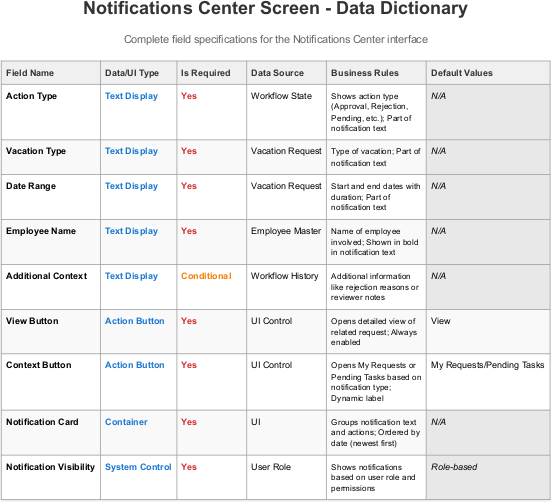
\includegraphics[width=0.8\textwidth]{Data-Dictionary/Screen-Data-Dictionaries/Notifications-Center-Screen-Data-Dictionary/Notifications-Center-Screen-Data-Dictionary-1.png}
\caption{Notifications Center Screen Data Dictionary}
\label{fig:notifications-center-data-dict}
\end{figure}

\subsubsection{Print Single Transaction Report Data Dictionary}
\begin{figure}[H]
\centering
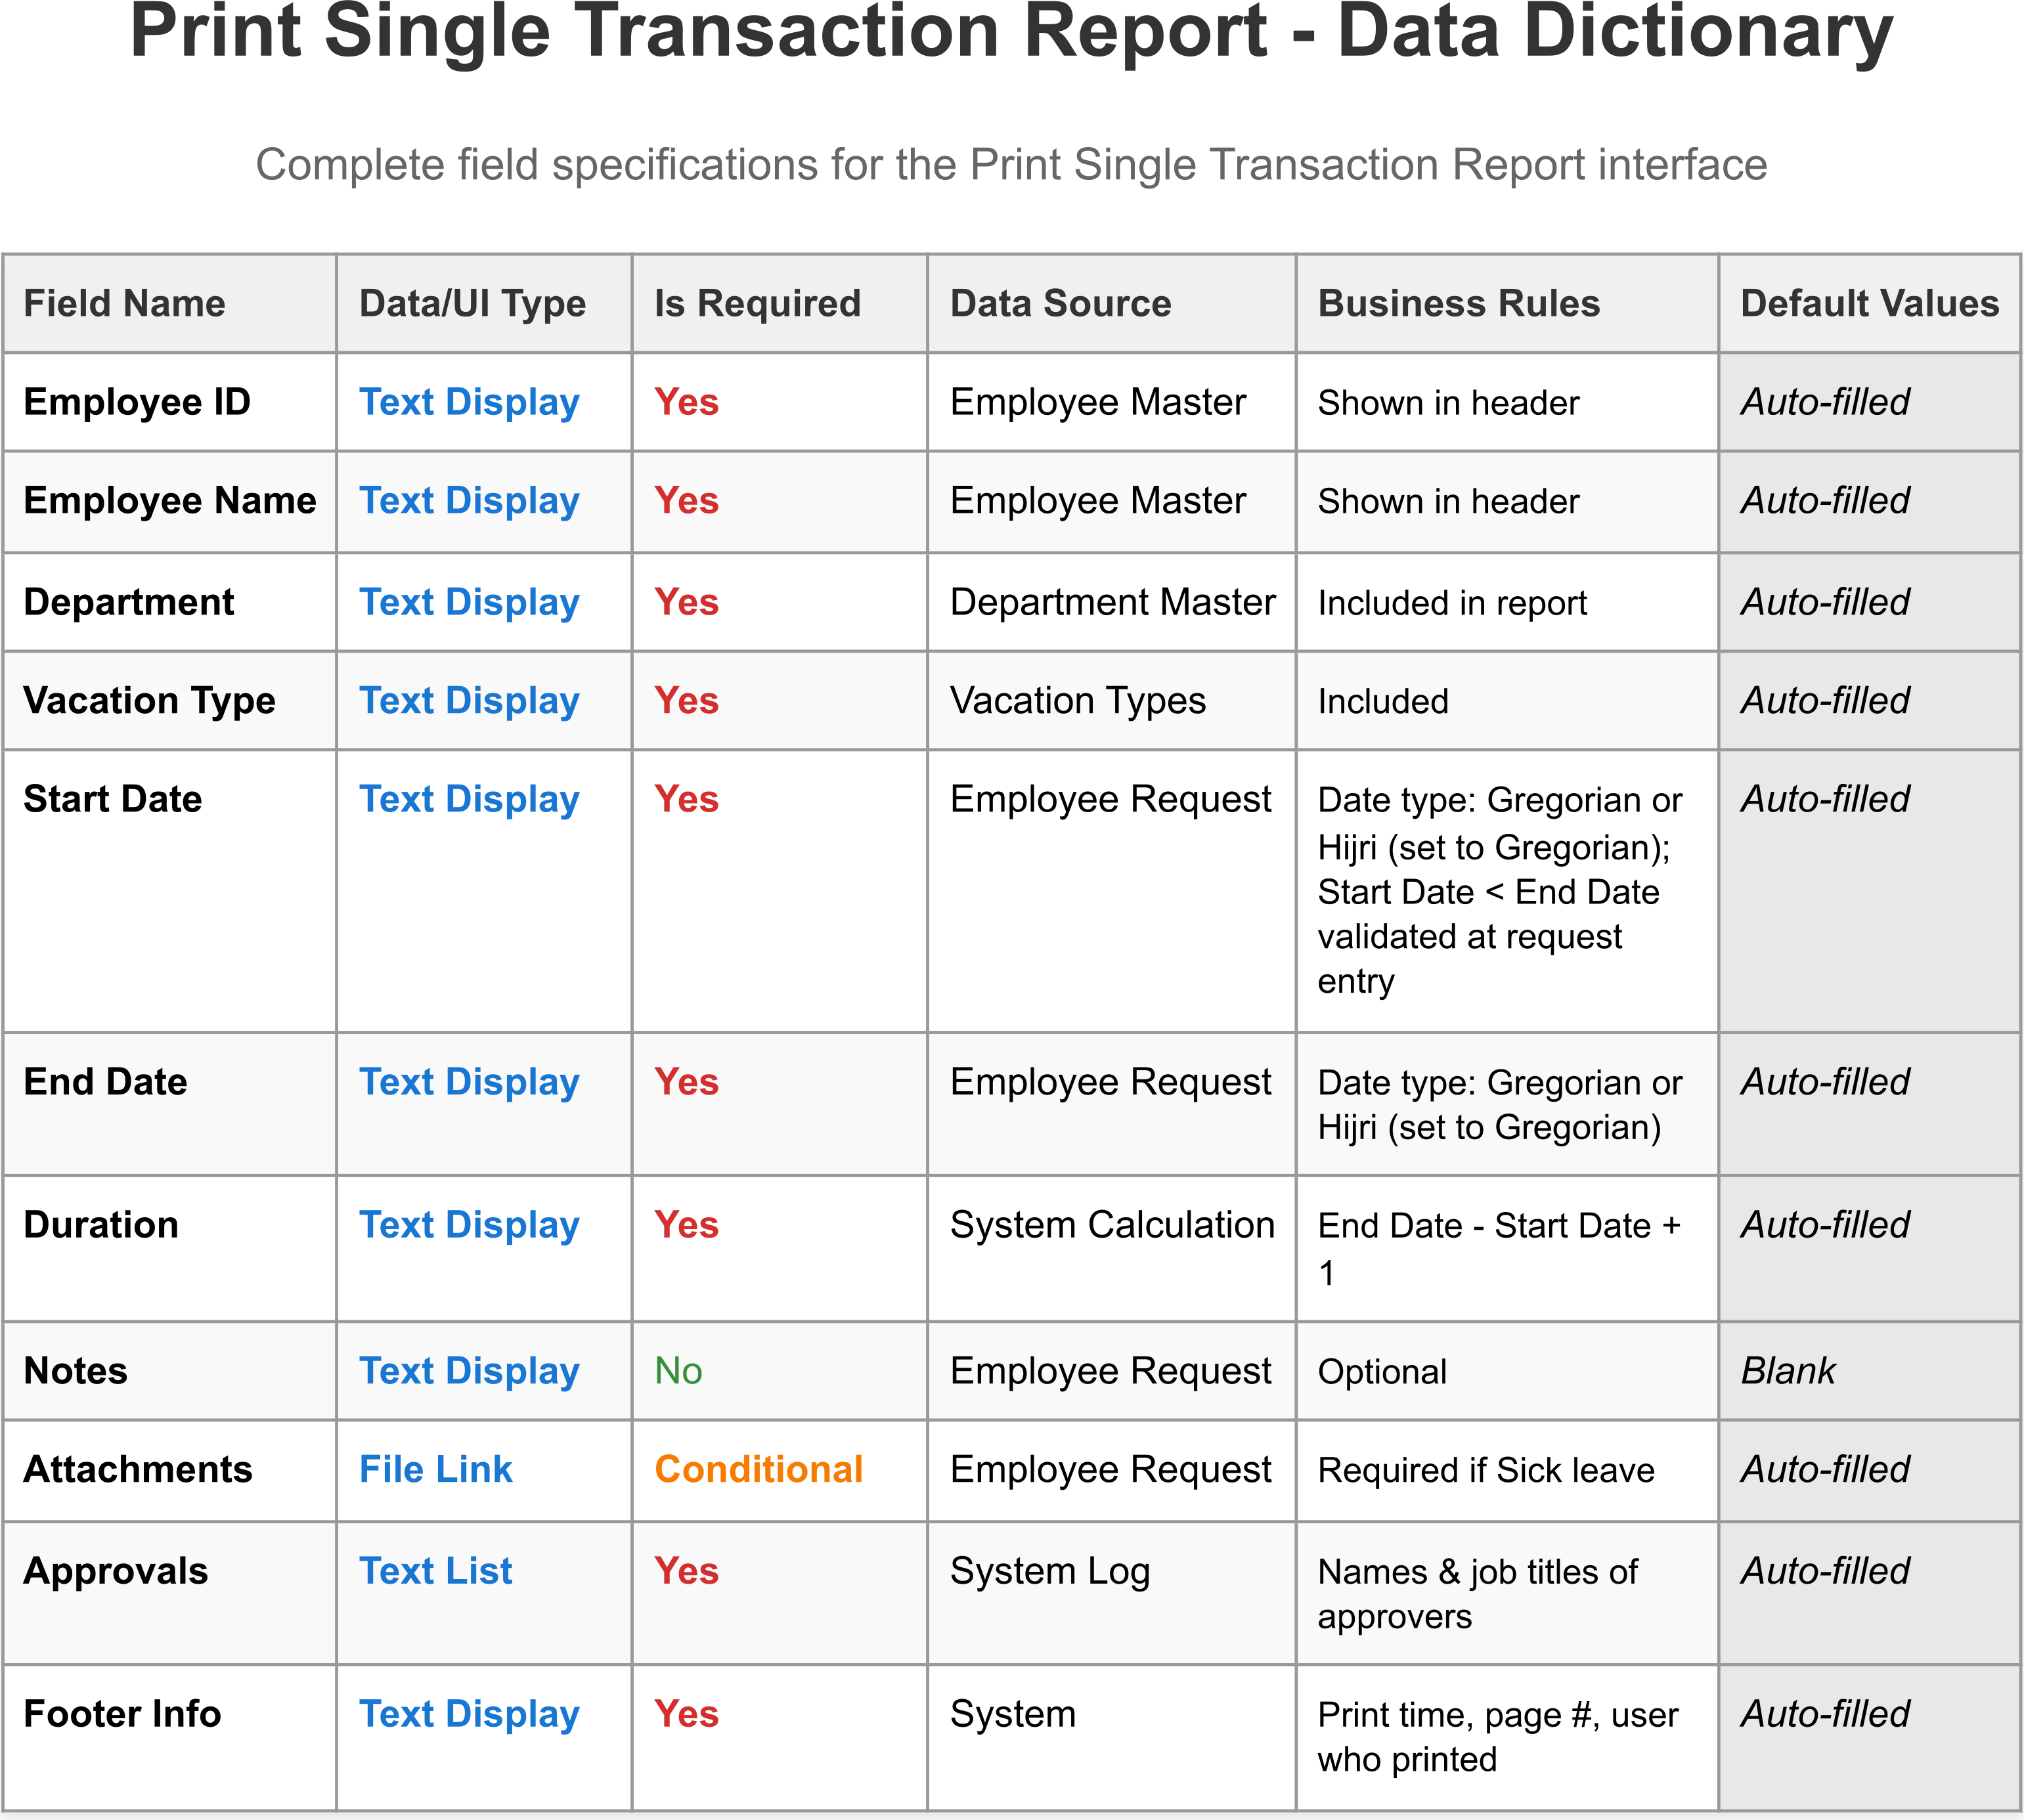
\includegraphics[width=0.8\textwidth]{Data-Dictionary/Screen-Data-Dictionaries/Print-Single-Transaction-Report-Data-Dictionary/Print-Single-Transaction-Report-Data-Dictionary-1.png}
\caption{Print Single Transaction Report Data Dictionary}
\label{fig:print-single-transaction-data-dict}
\end{figure}

\subsubsection{Print Comparative Annual Report Data Dictionary}
\begin{figure}[H]
\centering
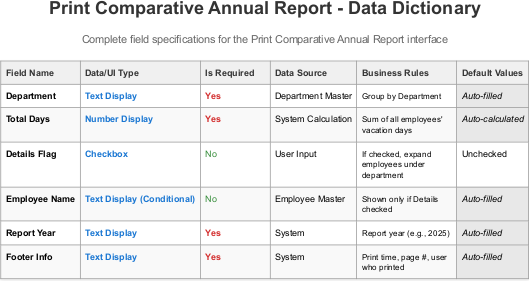
\includegraphics[width=0.8\textwidth]{Data-Dictionary/Screen-Data-Dictionaries/Print-Comparative-Annual-Report-Data-Dictionary/Print-Comparative-Annual-Report-Data-Dictionary-1.png}
\caption{Print Comparative Annual Report Data Dictionary}
\label{fig:print-comparative-annual-data-dict}
\end{figure}

\subsection{System Messages Table}
The system includes a comprehensive message table for all user communications and error messages.

\begin{figure}[H]
\centering
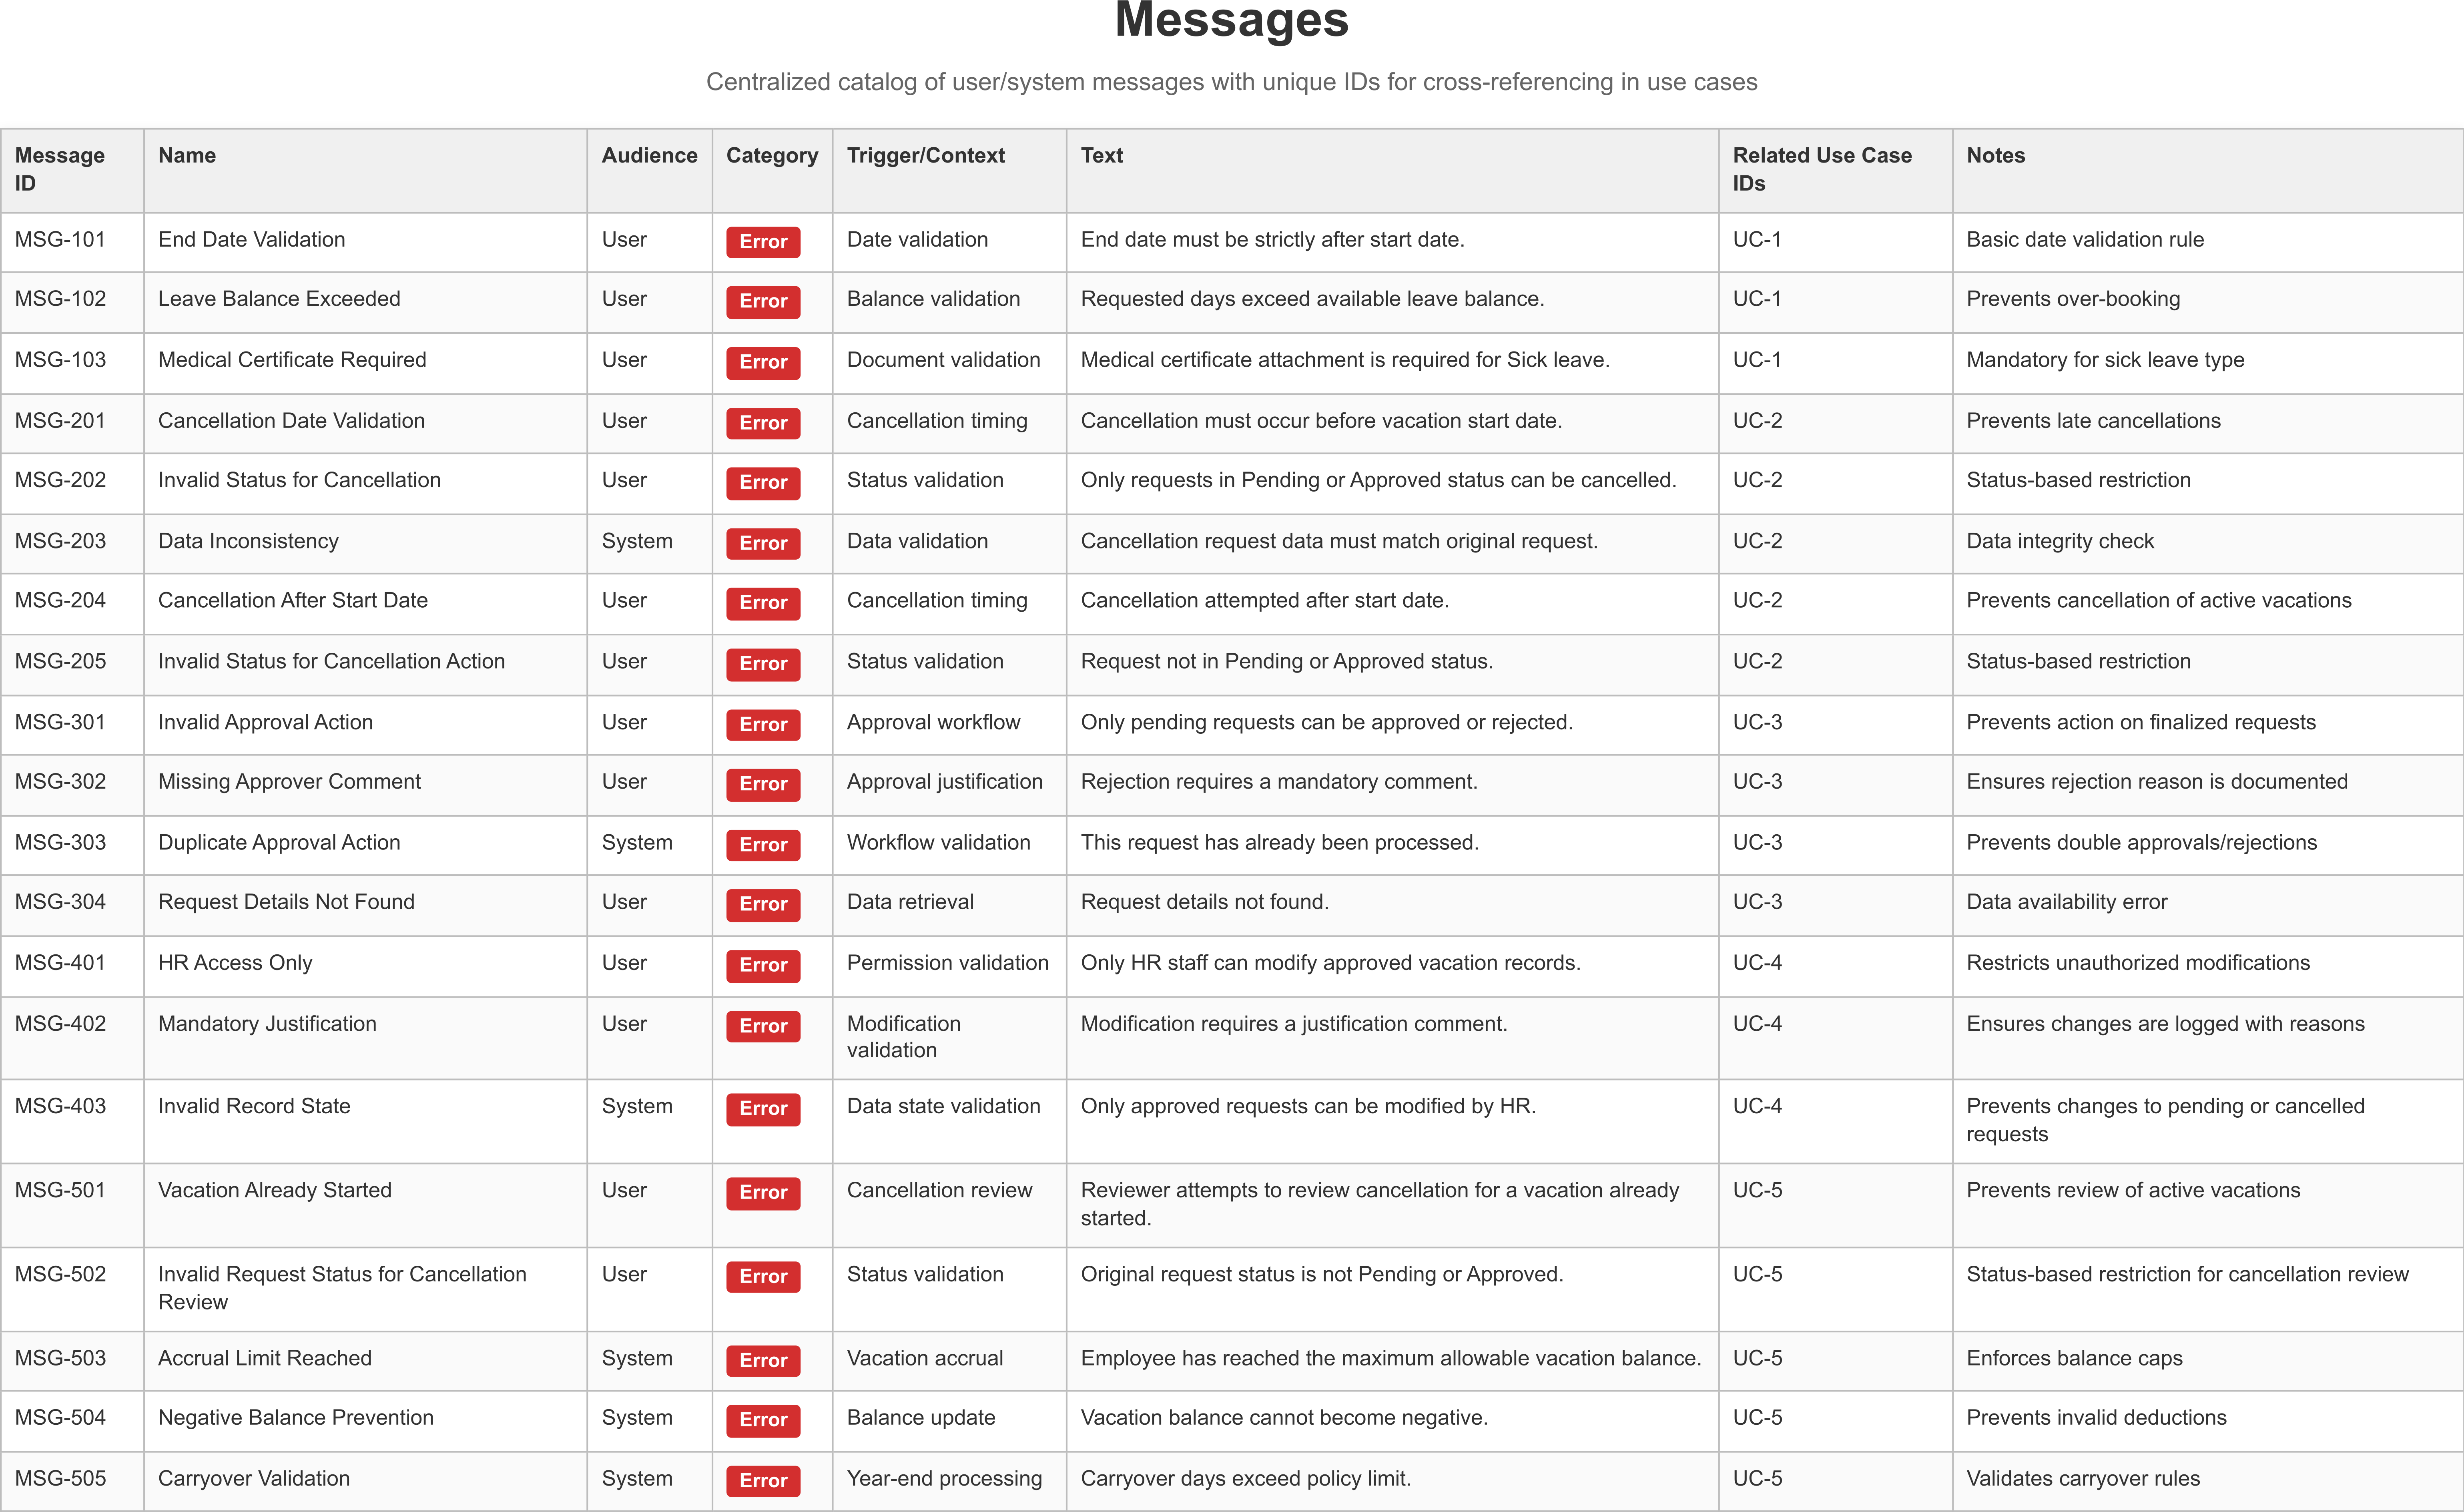
\includegraphics[width=1\textwidth]{Use-Cases/Messages-Table/Messages-Table-1.png}
\caption{System Messages Table - Part 1}
\label{fig:messages-table-1}
\end{figure}

\begin{figure}[H]
\centering
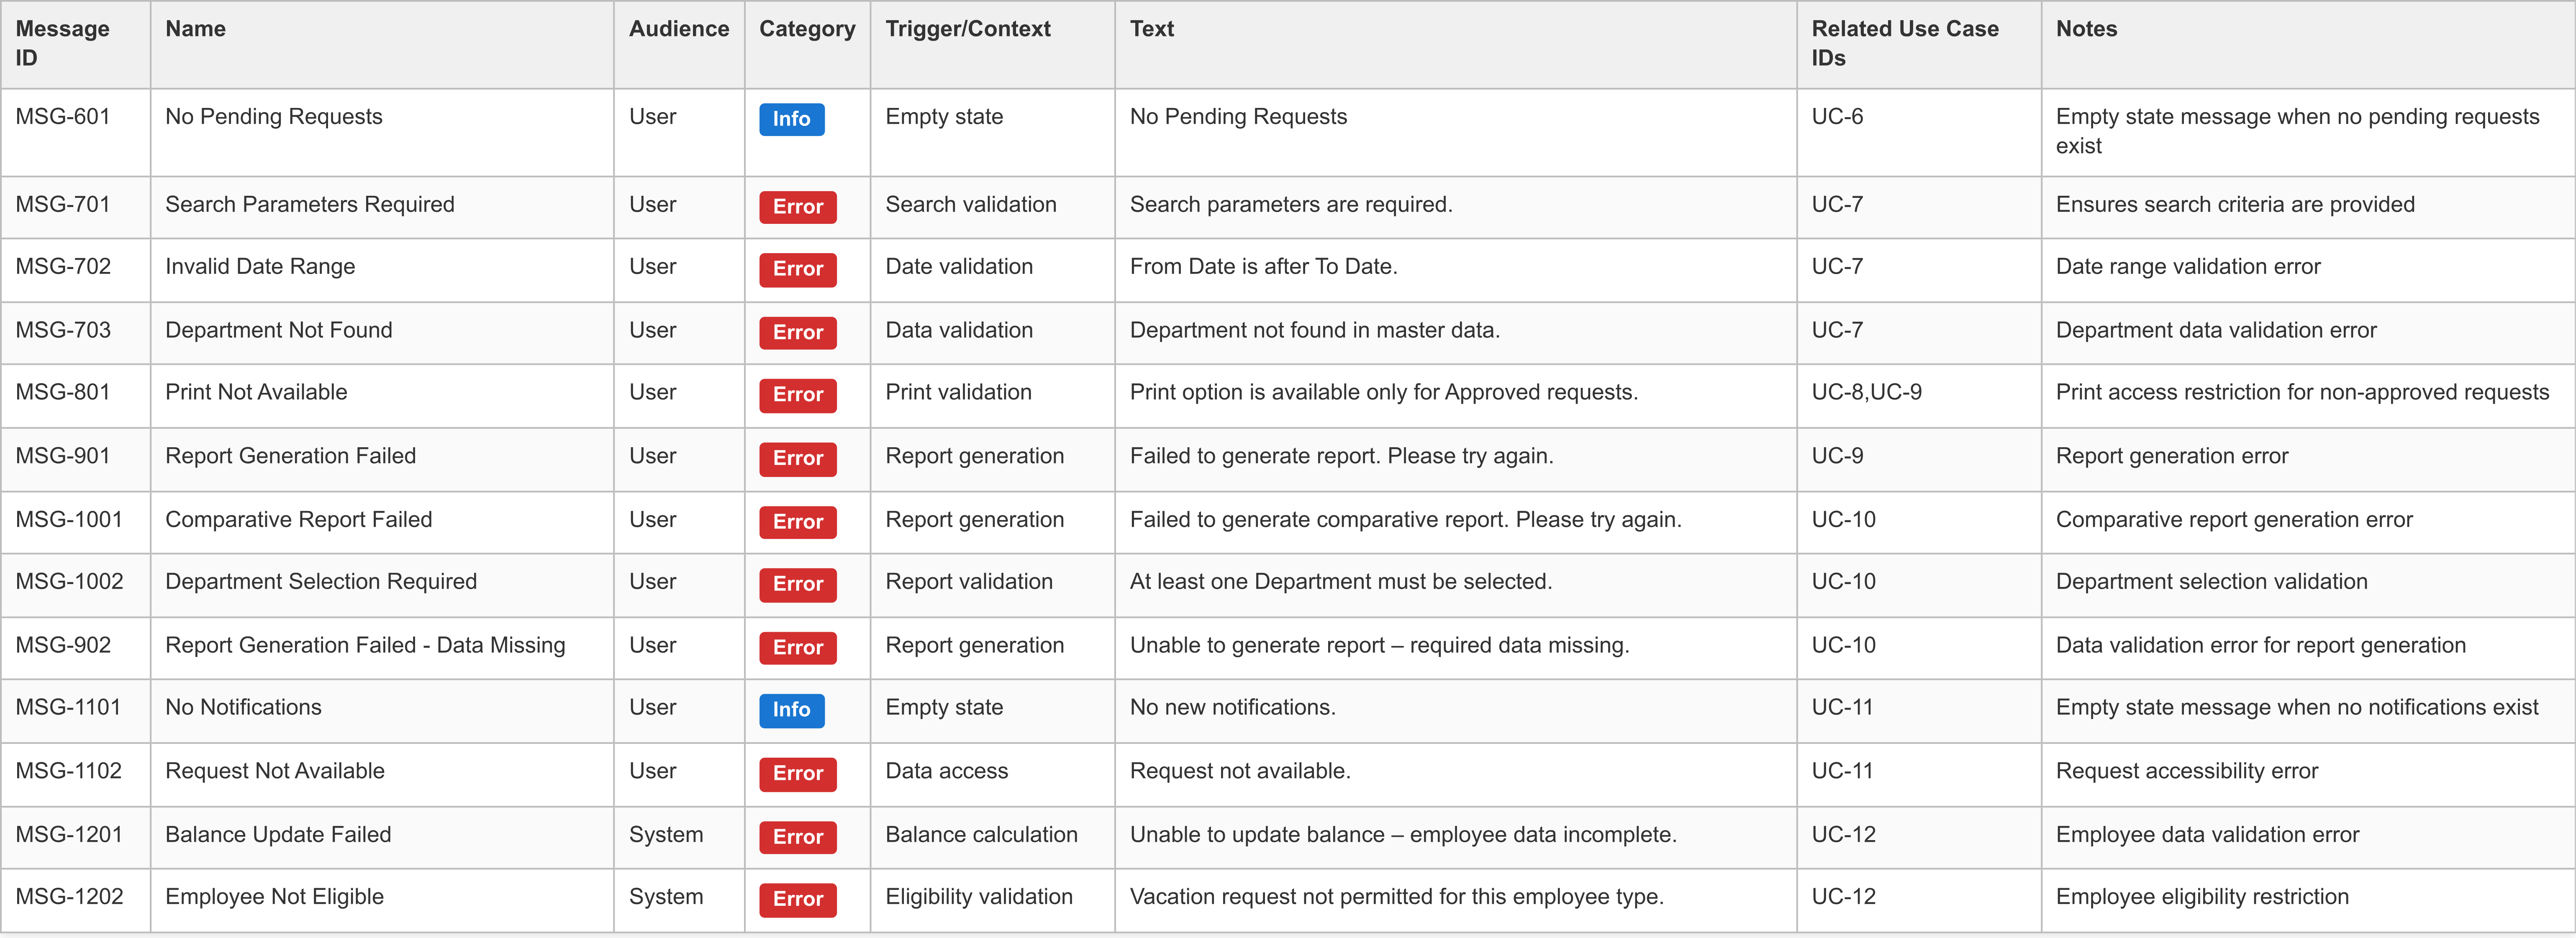
\includegraphics[width=1\textwidth]{Use-Cases/Messages-Table/Messages-Table-2.png}
\caption{System Messages Table - Part 2}
\label{fig:messages-table-2}
\end{figure}

\section{Non-Functional Requirements}

\subsection{Performance Requirements}
\begin{itemize}
    \item \textbf{Response Time}: Page load < 3 seconds
    \item \textbf{Throughput}: Support 100+ concurrent users
    \item \textbf{Availability}: 99.5\% uptime during business hours
    \item \textbf{Scalability}: Support up to 1000 employees
    \item \textbf{PDF Generation}: < 5 seconds for standard reports
\end{itemize}

\subsection{Security Requirements}
\begin{itemize}
    \item \textbf{Authentication}: Secure login with session management
    \item \textbf{Authorization}: Role-based access control
    \item \textbf{Data Protection}: Encrypt sensitive employee information
    \item \textbf{Audit Trail}: Log all system activities
    \item \textbf{Input Validation}: SQL injection and XSS prevention
\end{itemize}

\subsection{Usability Requirements}
\begin{itemize}
    \item \textbf{User Interface}: Intuitive, responsive design
    \item \textbf{Accessibility}: WCAG 2.1 AA compliance
    \item \textbf{Multi-language}: Arabic and English support
    \item \textbf{Mobile Support}: Responsive design for all devices
    \item \textbf{Error Handling}: Clear, actionable error messages
\end{itemize}

\subsection{Reliability Requirements}
\begin{itemize}
    \item \textbf{Error Handling}: Graceful error messages
    \item \textbf{Data Integrity}: Prevent data corruption
    \item \textbf{Backup}: Daily automated backups
    \item \textbf{Recovery}: 4-hour maximum recovery time
    \item \textbf{Validation}: Comprehensive business rule validation
\end{itemize}

\section{Business Rules and Logic}

\subsection{Vacation Policy Rules}
\begin{itemize}
    \item \textbf{Standard Entitlement}: 21 days per year
    \item \textbf{Extended Entitlement}: 30 days for employees with >10 years service or >50 years old
    \item \textbf{Leave Types}: Annual and Sick leave only
    \item \textbf{Unused Days}: Forfeited annually, no carryover
    \item \textbf{Emergency Exceptions}: Supported via flags even with zero balance
    \item \textbf{Trainee Restrictions}: Cannot submit vacation requests
\end{itemize}

\subsection{Approval Workflow Rules}
\begin{itemize}
    \item \textbf{Approval Hierarchy}: Employee → Direct Manager → HR → General Manager
    \item \textbf{Escalation}: Automatic after 2 days of delay
    \item \textbf{Balance Update}: Only after General Manager approval
    \item \textbf{Rejection Reasons}: Required for all rejections
    \item \textbf{Notification}: Sent for all status changes
    \item \textbf{No Modification}: Submitted requests cannot be modified
\end{itemize}

\subsection{Validation Rules}
\begin{itemize}
    \item \textbf{Date Validation}: No past dates, logical date ranges
    \item \textbf{Overlap Prevention}: No conflicting requests for same employee
    \item \textbf{Balance Checking}: Requested days < available balance
    \item \textbf{Attachment Requirements}: Mandatory for sick leave
    \item \textbf{Cancellation Rules}: Only before vacation start date
    \item \textbf{Status Validation}: Only Pending or Approved requests can be cancelled
\end{itemize}

\section{Technical Specifications}

\subsection{Technology Stack}
\begin{itemize}
    \item \textbf{Frontend}: HTML5, CSS3, JavaScript, React/Angular
    \item \textbf{Backend}: Node.js/Python/Java
    \item \textbf{Database}: SQL Server/MySQL/PostgreSQL
    \item \textbf{PDF Generation}: jsPDF, iText, or similar
    \item \textbf{Authentication}: JWT, OAuth, or session-based
    \item \textbf{Workflow Engine}: Custom implementation or BPMS
\end{itemize}

\subsection{Performance Specifications}
\begin{itemize}
    \item \textbf{Response Time}: < 3 seconds for page loads
    \item \textbf{Database Queries}: < 1 second for standard operations
    \item \textbf{PDF Generation}: < 5 seconds for standard reports
    \item \textbf{Concurrent Users}: Support for 100+ simultaneous users
    \item \textbf{File Upload}: Support for multiple file types and sizes
\end{itemize}

\subsection{Security Specifications}
\begin{itemize}
    \item \textbf{Encryption}: AES-256 for sensitive data
    \item \textbf{Password Policy}: Minimum 8 characters, complexity requirements
    \item \textbf{Session Management}: Secure session handling with timeout
    \textbf{Input Validation}: SQL injection and XSS prevention
    \item \textbf{File Security}: Secure file upload and storage
\end{itemize}

\section{Testing Requirements}

\subsection{Functional Testing}
\begin{itemize}
    \item \textbf{Unit Testing}: Individual component testing
    \item \textbf{Integration Testing}: Module interaction testing
    \item \textbf{System Testing}: End-to-end functionality testing
    \item \textbf{User Acceptance Testing}: Stakeholder validation
    \item \textbf{Workflow Testing}: Approval process validation
\end{itemize}

\subsection{Non-Functional Testing}
\begin{itemize}
    \item \textbf{Performance Testing}: Load and stress testing
    \item \textbf{Security Testing}: Vulnerability assessment
    \item \textbf{Usability Testing}: User experience validation
    \item \textbf{Compatibility Testing}: Cross-browser and device testing
    \item \textbf{PDF Generation Testing}: Report output validation
\end{itemize}

\section{Deployment and Maintenance}

\subsection{Deployment Strategy}
\begin{itemize}
    \item \textbf{Environment Setup}: Development, testing, production
    \item \textbf{Database Migration}: Schema creation and data migration
    \item \textbf{User Training}: Comprehensive training program
    \item \textbf{Go-Live Plan}: Phased rollout strategy
    \item \textbf{Integration Testing}: External system integration validation
\end{itemize}

\subsection{Maintenance Requirements}
\begin{itemize}
    \item \textbf{Regular Updates}: Security patches and bug fixes
    \item \textbf{Performance Monitoring}: System health tracking
    \item \textbf{Backup Verification}: Regular backup testing
    \item \textbf{User Support}: Help desk and documentation
    \item \textbf{Policy Updates}: Vacation policy configuration management
\end{itemize}

\section{Appendices}

\subsection{Appendix A: Glossary}
\begin{itemize}
    \item \textbf{Vacation}: Time off from work for personal reasons
    \item \textbf{Leave Balance}: Remaining vacation days available
    \item \textbf{Approval Workflow}: Process for request authorization
    \item \textbf{Escalation}: Automatic forwarding of delayed requests
    \item \textbf{Attachments}: Supporting documents for requests
    \item \textbf{Entitlement}: Annual vacation days allocation
    \item \textbf{Trainee}: Employee in training status, ineligible for vacation
\end{itemize}

\subsection{Appendix B: Data Models}
\begin{itemize}
    \item Entity-Relationship Diagrams
    \item Database Schema Definitions
    \item API Specification Documents
    \item Integration Interface Definitions
    \item Master Data Entity Definitions
\end{itemize}

\subsection{Appendix C: Wireframe Images}
\begin{itemize}
    \item Vacation Request Screen (Web \& Mobile)
    \item Vacation Cancellation Screen (Web \& Mobile)
    \item Review Screens (Web \& Mobile)
    \item Inquiry and Search Screens
    \item Report Layouts
    \item Dashboard and Analytics Screens
    \item Notifications Center
\end{itemize}

\subsection{Appendix D: State Diagrams}
\begin{itemize}
    \item Vacation Request State Flow
    \item Approval Workflow States
    \item Cancellation Process States
    \item System Status Transitions
    \item Employee Balance Update States
\end{itemize}

\subsection{Appendix E: Workflow Diagrams}
\begin{itemize}
    \item Basic Vacation Request Flow
    \item Escalation to Sponsor Flow
    \item Resubmission After Rejection Flow
    \item Cancellation Approval Flow
    \item Multi-level Approval Process
\end{itemize}

\subsection{Appendix F: Use Case Templates}
\begin{itemize}
    \item Standard Use Case Template
    \item Use Case Documentation Standards
    \item Business Rule Definition Format
    \item Exception Handling Documentation
\end{itemize}

\section{Document Approval}

\subsection{Stakeholder Signatures}
\begin{table}[H]
\centering
\begin{tabular}{|p{4cm}|p{4cm}|p{4cm}|}
\hline
\textbf{Name} & \textbf{Role} & \textbf{Signature \& Date} \\
\hline
 & Project Manager &  \\
\hline
 & Technical Lead &  \\
\hline
 & Business Analyst &  \\
\hline
 & Stakeholder Representative &  \\
\hline
\end{tabular}
\caption{Document Approval Signatures}
\end{table}

\subsection{Version History}
\begin{table}[H]
\centering
\begin{tabular}{|p{2cm}|p{3cm}|p{4cm}|p{3cm}|}
\hline
\textbf{Version} & \textbf{Date} & \textbf{Changes} & \textbf{Author} \\
\hline
1.0 & Initial & Initial SRS Document & System Analyst \\
\hline
2.0 & \today & Complete rewrite with all project materials & System Analyst \\
\hline
\end{tabular}
\caption{Document Version History}
\end{table}

\end{document}
